% ------------------------------------------------------------------------
% ------------------------------------------------------------------------
% abnTeX2: Modelo de Trabalho Acadêmico (tese de doutorado, dissertação de
% mestrado e trabalhos monográficos em geral) em conformidade com
% as normas da ABNT
% ------------------------------------------------------------------------
% ------------------------------------------------------------------------

\documentclass[english, 
               brazil, 
               msc] %Opções msc (Mestrado)
               {ppgpi-abntex2}
% Geração de dummy text
% Retirar para a versão final do documento


%Compila o indíce
\makeindex

\begin{document}

% Seleciona o idioma do documento (conforme pacotes do babel)
\selectlanguage{brazil}

% Retira espaço extra obsoleto entre as frases.
\frenchspacing 

% ----------------------------------------------------------
% ELEMENTOS PRÉ-TEXTUAIS
% ----------------------------------------------------------

\pretextual


\titulo{Programa Empreenda Agro Sustentável como mecanismo indutor de inovação}
\orientador{Prof. Dr. Francisco Sandro Rodrigues Holanda}
\author{Luiz Diego Vidal Santos}


\curso{Ciência da Propriedade Intelectual}

\imprimircapa

\imprimirfolhaderosto

%\imprimirfichacatalografica
%\imprimirfolhadeaprovacao
\begin{dedicatoria}
   \vspace*{\fill}
   \centering
   \noindent
   \textit{Dedico este trabalho de mestrado a toda a minha família, noiva, amigos e \\
   professores que me deram o apoio necessário para chegar até aqui.} \vspace*{\fill}
\end{dedicatoria}
% ---
\begin{agradecimentos}

A minha família pelo apoio, colaboração, amor, empenho e paciência. 

Aos colegas de curso pela amizade, companheirismo, espontaneidade e alegria ao longo desses anos de convivência.

E, finalmente, a Deus pela fé e força depositadas em mim para que eu pudesse enfrentar este curso e conseguir concluí-lo.
\end{agradecimentos}
% ---
\begin{epigrafe}[]
    \vspace*{\fill}
	\begin{flushright}
	
		\textit{"A plenitude da atividade humana é alcançada somente quando nela coincidem, se acumulam,\\ se exaltam e se mesclam o trabalho o estudo e o jogo; isto é,  quando nós \\ trabalhamos, aprendemos e nos divertimos, tudo ao mesmo tempo."\\
				\textbf{Domenico de Masi}}
		
	\end{flushright}
\end{epigrafe}
% ---

, ,  

% resumo em português
\setlength{\absparsep}{18pt} % ajusta o espaçamento dos parágrafos do resumo
\begin{resumo}

 %Melhorar esse resumo para projetos!!!

Ser empreendedor não significa apenas ter seu próprio negócio, o empreendedorismo está ligado às ações e capacidades individuais, ou seja, possuir características empreendedoras é ser capaz de criar, modular e sustentar ideias inovadoras globalmente, assim as ideias normalmente estão ligadas à inovação algo que transcende o comum. Algumas ferramentas tais como workshops, jornadas, cursos, palestras podem ser usadas para difusão do comportamento empreendedor tanto em órgãos privados como em instituições de ensino, ou seja, incutir novas ações empreendedoras no sentido comercial, nas áreas industriais e agrícolas que sejam sustentáveis. Faz-se necessário, então, a construção de um cenário favorável ao desenvolvimento da cultura empreendedora no ambiente acadêmico, principalmente nas ciências agrárias. Para construção deste senário, muitas nações estão buscando promover a atividade empreendedora, utilizando para isto programa educacionais promovidos nos meios acadêmicos alcançando um importante público os jovens. Assim, torna-se evidente que o sistema educacional que promova o desenvolvimento das competências empreendedoras tem um importante papel a cumprir para com a causa empreendedora. Neste sentido, este estudo estudo tem como objetivo, identificar de forma analítica a inovação sustentável e a eficácia da promoção empreendedora por meio de uma ação de educação com vistas aos negócios rurais, tendo como ferramenta promotora o Programa Empreenda Agro Sustentável. O Programa visa buscar o engajamento dos alunos para o desenvolvimento de novos negócios direcionados ao setor agrícola, podendo este experimento também direcionar futuras pesquisas científicas focadas em produtos capazes de satisfazer às novas demandas, de forma eficiente e sustentável. A metodologia de natureza quantitativa exploratória e de estudo de caso, foi utilizada para avaliar quantitativamente o Programa Empreenda AGRO Sustentável, com análise dos dados, que foram coletados por meio da técnica quantitativa “survey” tendo como base o estudo GUESS. A ferramenta de promoção prática do exercício do comportamento empreendedor “Programa Empreenda AGRO Sustentável", foi conduzida buscando a disseminação do empreendedorismo junto aos acadêmicos do Centro de Ciências Agrárias Aplicadas da Universidade Federal de Sergipe – UFS. Foram conduzidos quatro Workshops, planejados de forma sistemática e interativa, sendo aplicadas ferramentas para modelagem de negócios como Design Thinking visando despertar ideias de startups em oficinas interdisciplinares fomentando desta forma a construção de Mínimos Produtos Comercialmente Viáveis (MCVP).

\textbf{Palavras-chave}: Empreendedorismo; Competências empreendedoras; Negócios sustentáveis; Propriedade Intelectual; Projeto de Extensão.
\end{resumo}


% resumo em inglês
\setlength{\absparsep}{18pt} % ajusta o espaçamento dos parágrafos do resumo
\begin{resumo}[Abstract]
 \begin{otherlanguage*}{english}
   
Being an entrepreneur does not just mean having your own business, entrepreneurship is linked to individual actions and capabilities to create, modulate and sustain innovative ideas globally. Thus, ideas are usually linked to innovation, something that transcends the ordinary. Some tools such as workshops, seminars, courses, lectures can be used to disseminate entrepreneurial behavior both in private bodies and in educational institutions, in order to instill new sustainable entrepreneurial actions, in the commercial sense, in the industrial and agricultural areas in the academic environment. . It is necessary, then, to build a favorable scenario for the development of entrepreneurial culture in the academic environment, mainly in the agricultural sciences. In this context, many nations are seeking to promote entrepreneurial activities, using educational programs promoted in academic circles to reach an important young audience. In this sense, this study aims to identify, in an analytical way, sustainable innovation and the effectiveness of encouraging entrepreneurship through an educational action aimed at rural businesses, using the Empreenda AGRO Sustentável Program as a promoting tool. The Program aims to seek student engagement for the development of new businesses aimed at the agricultural sector, and this experiment can also direct future scientific research focused on products capable of satisfying new demands, in an efficient and sustainable manner. The methodology of quantitative exploratory nature and case study was used to quantitatively evaluate the Empreenda AGRO Sustentável Program with data collection using the “survey” technique based on the GUESS study. The tool for the practical promotion of entrepreneurial behavior “Programa Empreenda AGRO Sustentável” was conducted seeking the dissemination of entrepreneurship among academics at the Center for Applied Agricultural Sciences at the Federal University of Sergipe (UFS). Four workshops were planned and executed in a systematic and interactive way , in which methodologies and tools for business modeling such as Design Thinking were applied in order to awaken ideas from startups through interdisciplinary workshops, thus promoting the construction of Minimum Commercially Viable Products (MCVP). Sustainable and based on the application of active methodologies, 15 teams discussed and matured ideas in models of startups, resulting in scalable and negotiable business models aimed at the rural environment. As a result, the research found that the participating students had a strong positive influence on the intention entrepreneur a and self-efficacy for entrepreneurship. In addition, the research demonstrated that the students involved in the course of the program positively evolved the entrepreneurial dimensions studied, thus influencing the development of new businesses planned in the pre-acceleration stage, and found greater security for the next step, which is the acceleration of their business plans, gaining autonomy, seeking new opportunities as proactive professionals in the job market.

 \textbf{Keywords}:Sustainable business, Intellectual Property, Extension Project.
 \end{otherlanguage*}
\end{resumo}
    
 %Lista de Figuras %%%%%%%%%%%%%%
    \pdfbookmark[0]{\listfigurename}{lof}
     \listoffigures*
   \cleardoublepage

% Lista de Tabelas %%%%%%%%%%%%%
    \pdfbookmark[0]{\listtablename}{lot}
     \listoftables*
    \cleardoublepage

\cleardoublepage
   
% ---
% inserir lista de abreviaturas e siglas
% ---

\begin{siglas}
    
  	\item[EE]{Educação Empreendedora}
  	%\item[DB]{Data Base}
  	\item[INPI]{Instituto Nacional da Propriedade Intelectual}
  	\item[PI]{Propriedade Intelectual}
  	\item[GUESSS]{\textit{Global University Entrepreneurial Spirit Students Survey}}
  	\item[EAESP]{Escola de Administração de Empresas de São Paulo}
  	\item[FGV]{Fundação Getúlio Vargas}
  	\item[ABP]{ Aprendizagem Baseada em Problemas}

\end{siglas}
% ---
%% ---
% inserir lista de símbolos
% ---

\begin{simbolos}
  \item[$ \sum  $] Letra grega Sigma
  \item[$ \int $] Integral
  \item[$ \omega $] Letra grega ómega
\end{simbolos}
% ---
\pdfbookmark[0]{\contentsname}{toc}
\tableofcontents*
\cleardoublepage

% ----------------------------------------------------------
% ELEMENTOS TEXTUAIS
% ----------------------------------------------------------
\textual
\chapter{INTRODUÇÃO}

O empreendedorismo  pode ser compreendido como a arte de fazer acontecer com criatividade e motivação. As vezes é visto como um vislumbre de esperança que pode trazer alguma contribuição para a melhoria da dinâmica e do desempenho econômico, especificamente na criação de emprego para profissionais recém-formados. Estes profissionais, geralmente, buscam treinamentos educacionais adicionais que visam aprimorar a visão estratégica de negócios, capacidade de liderança, além de preparar os profissionais para trabalhar com novas tecnologias, uma vez que este é o perfil requerido pelas grandes empresas e startups no agronegócio. No entanto, o empreendedorismo no setor agrícola é, em certas circunstâncias, visto como algo incompatível ou, pelo menos, difícil de implementar e ministrar.

Mais estudos científicos no campo da educação direcionados ao desenvolvimento da intenção empreendedora podem fornecer contribuições interessantes no sentido de destacar novas ideias dentro do setor agrícola. Nesse contexto, o objetivo desse trabalho foi identificar de forma analítica a inovação sustentável e a eficácia da promoção empreendedora por meio de uma ação de educação com vistas aos negócios rurais, tendo como ferramenta promotora o Programa Empreenda Agro Sustentável.



\section{JUSTIFICATIVA}

As oportunidades de trabalho para os novos profissionais atuantes na área das ciências agrárias vêm mudando, se transformando numa busca pela valorização das capacidades e competências ocupacionais. Busca-se cada vez mais a autoeficácia, a promoção de direitos de cidadania, associativismo político, responsabilidade social e ambiental, consideração, respeito às diversidades étnicas e culturais. Para tal, a academia tem um papel importante neste contexto, que é o de fomentar e oportunizar o surgimento destas competências. Dentro deste contexto, a capacidade de implementar inovação, especialmente a disruptiva é fundamental ao progresso do crescimento e manutenção da carreira do profissional das ciências agrárias no novo mercado de serviços e produtos. 


De acordo com \citeonline{tarapanoff_monitoramento_2016}, existe um cenário favorável para os negócios rurais que buscam a sustentabilidade econômica e ambiental. Nesse sentido, o Brasil deve buscar trilhar um caminho seguro em relação à sustentabilidade do agronegócio. Buscando, desta forma, consonância com as melhores práticas no uso dos recursos ambientais e a produção agrícola, cumprimento às regras ambientais, como por exemplo a Agenda 2030, que prevê o uso consciente e sustentável dos recursos naturais e, tomando medidas urgentes sobre as mudanças climáticas individuais quanto institucionais, \cite{filho_documentos_2017}. O desenvolvimento sustentável pode ser definido, segundo \cite{lara_ideologia_2017}, como um negócio socialmente responsável e ecologicamente correto, mas invariavelmente viável em termos financeiros.


Concomitantemente a esta realidade, existe uma lacuna na formação profissional durante o ensino superior dos estudantes de ciências agrárias no que se refere à adoção de uma cultura empreendedora, \cite{araujo_educacao_2019}. Não tem sido possibilitado aos acadêmicos a oportunidade de gerar inovação tecnológica sustentável, inclusive para a aplicação prática dos conhecimentos adquiridos. Da mesma maneira, para que uma ideia inovadora alcance o sucesso desejado é preciso muito mais que o conhecimento técnico. Deve-se ser disponibilizado aos futuros profissionais/empreendedores, treinamento na formulação das ideias em etapas direcionadas e adequadamente orientadas. Para que um negócio sustentável possa ter sucesso é preciso mais do que uma ideia inovadora, deve-se ter o meio e profissionais capacitados para tal. 


O Relatório da Fundação \textit{Wing Marion Kauffman} afirma que as Startups criam uma média de 3 milhões de novas vagas de empregos anualmente e que, estes empreendimentos serão responsáveis pela criação de 60\% das ocupações laborais no mundo \cite{brasil_o_2017}. Atualmente estas categorias de negócios contribuem para o crescimento de diversas regiões geográficas, já que não se expandem apenas em tamanho, mas também em novos locais, além de incentivar o emprego em suas indústrias relacionadas. Supletivamente, como muitas dessas microempresas são responsáveis por desenvolver novas tecnologias e processos, elas também geram aumento de absorção do capital humano mais capacitado para gerenciamento empresarial.


Diante deste cenário, para que o aprendizado dos profissionais seja mais efetivo, surgem diversas abordagens e metodologias a serem assimiladas. Nesse contexto, deve existir uma maior produção de estudos e conteúdos sobre o empreendedorismo e os modelos educacionais que melhor se apliquem ao aprendizado, como ressalta \citeonline{dionello_educacao_2020}. É notória a urgência de se pesquisar o ensino em empreendedorismo de forma disciplinada no meio acadêmico. Por ser um tema de grande importância, a educação em empreendedorismo promovida no seio do ensino superior pode ser o caminho para o surgimento de inovações sustentáveis e economicamente viáveis, passíveis e escaláveis.

No contexto metodológico educacional, temos as metodologias ativas, que trazem a possibilidade de mudança da centralidade no docente (ensino) para o estudante (aprendizagem). Os métodos compreendem a educação como um processo que não é realizado por outrem, ou pelo próprio indivíduo, mas que acontece na interação entre pessoas através de sua vivência por palavras, ações e reflexões \cite{paiva_metodologias_2016}. Enquanto o método tradicional de ensino utiliza a transmissão de informações e concentra as atividades no docente, na metodologia ativa, os alunos ocupam a centralidade da educação e o conhecimento é construído de forma colaborativa. Sucintamente, as metodologias ativas podem transformar o processo de ensino na busca pelo comportamento empreendedor, como uma forma de enfrentar o modelo tradicional praticado e aceito ao longo dos anos.
 
As práticas ativas estimulam o reconhecimento das dificuldades do mundo atual, tornando os alunos aptos a intervir na promoção das transformações necessárias, a exemplo daquelas que se baseiam na reflexão e argumentação \cite{bezanilla_methodologies_2019}. Assim, o aluno torna-se protagonista da sua aprendizagem e autônomo no alcance dos seus objetivos incorporando seus valores e razões \cite{rubel_student_2016}.

Existem vários recursos, métodos e técnicas para alcançar o satisfatório comportamento empreendedor, como: uso de tecnologias digitais e aplicativos \cite{pereira_use_2020}, ensino híbrido e suas estratégias como sala de aula em rotação por estações, Aprendizagem Baseada em Problemas (ABP) \cite{souza_aprendizagem_2015}, situações-problema e estudos de hipóteses problemas, sala de aula invertida \cite{junior_sala_2016,branco_sala_2016}, uso de mapas mentais \cite{junior_percepcao_2018}, sala de aula compartilhada \cite{strack_por_2009}, estratégias de Design Thinking \cite{andrews_circular_2015}, Gamificação \cite{ogawa_avaliacao_2016}, projetos de extensão \cite{santos_projeto_2019}. Dentre tantas outras ferramentas do método ativo que podem facilitar o entendimento e a compreensão dos acadêmicos das Ciências Agrárias no contexto de um mercado de trabalho que se apresenta com um perfil voltado ao empreendedorismo.

O empreendedorismo é a habilidade de reunir esforços para transformar em realidade uma oportunidade, objetivando a satisfação pessoal do empreendedor e o lucro. Tal conceito define o empreendedorismo como uma prática constante das atividades rotineiras dos educandos. Desde a capacidade de resolução de problemas quanto a idealização de propostas capazes de inovar. Dentro desta dicotomia entre empreendedorismo e educação surge a “Educação em Empreendedorismo”, que é construída por práticas e dinâmicas idealizadas, buscando a melhoria na promoção do comportamento empreendedor \cite{martins_educacao_2016, morais_empreendedorismo_2018}, e resolução de problemas de forma sustentável e rápida.

\section{DELIMITAÇÕES DO ESTUDO}

Esta pesquisa está focada na dissonância entre a teoria e prática dos métodos educacionais e as grandes e contínuas mudanças do mercado de trabalho no meio rural. Este setor foi escolhido por estar contribuindo significativamente para a balança comercial do país, apresentando saldos positivos frequentes. Igualmente contribui, para a segurança alimentar do País e produção de produtos limpos e renováveis. O mercado emergente apresenta significativa contribuição para a empregabilidade da população no campo, invertendo cada vez mais o êxodo rural, porém, este mercado que absorve novos profissionais, exige que tais profissionais sejam capazes de lidar com o desenvolvimento tecnológico e a produção em larga escala. 

Em contraponto, o empreendedorismo atualmente se confunde com a Meritocracia. Tanto a meritocracia quanto o empreendedorismo caminham juntos no cerne do movimento de individualização no mundo das ocupações laborais \cite{costa_novo_2019}. Os dois projetam imagens individuais de labor e sucesso, em que a capacidade individual somada às oportunidades gera resultados positivos junto ao mercado de trabalho. Porém, o Empreendedorismo derivado da educação em empreendedorismo, proposto neste projeto, surge atrelado às técnicas e aos métodos capazes de facilitar e validar as propostas empreendedoras,ou seja um programa que visa o incentivo às práticas empreendedoras de forma sistemática e coerente.

Visando compreender o comportamento empreendedor nos alunos dos cursos do Centro de Ciências Agrárias Aplicadas (CCAA) da Universidade Federal de Sergipe (UFS), foi definida a população para esta pesquisa de 1.453 discentes dos cursos do CCAA da UFS que refletem os dados contidos no relatório estatístico de matrículas 2017 da instituição, dos cursos: Engenharia Agronômica, Engenharia Agrícola, Zootecnia, Engenharia Florestal, Medicina Veterinária e Engenharia de Pesca. A amostra final compreendeu 120 discentes que participaram do Programa Empreenda Agro Sustentável.

As atividades foram desenvolvidas em quatro workshops, que trabalharam metodologias ativas, oficinas, palestras tendo em conta a promoção da aprendizagem significativa e colaborativa. Durante os módulos do projeto (workshops), os participantes testaram seus insights para que novas requisições fossem realizadas e/ou que erros nos planejamentos fossem encontrados e, consequentemente, debatidos e mitigados. Depois que todas as Sprints (atividades dos três workshops) foram finalizadas, ou seja, que todos os módulos foram abordados, foi iniciado um ciclo de apresentações e desenvolvimento da habilidade de apresentação e demonstração dos produtos por apresentações sumárias (Pitchs). 

O programa trouxe como principais benefícios: 

\begin{itemize}
\item{Promoção do desenvolvimento pessoal, econômico, social no meio rural através da oportunidade de acesso às alternativas de produção de renda;}
\item{Criação de oportunidade em trabalhar com o que realmente gosta e vencer os entraves do mercado econômico;}
\item{Autonomia e liberdade para conduzir o próprio talento, porém, orientado por metodologias específicas;}
\item{Valores e inspiração para os novos empreendedores no ambiente agrário;}
\item{Ensino de como lidar com os fracassos e frustrações, sabendo como os contornar;}
\item{Ensino de estratégias de organização de ideias ou carreiras buscando a receita positiva;}
\end{itemize}



Diversos experimentos sobre o empreendedorismo na América Latina têm utilizado \textit{Surveys} exploratórios realizados em residências ou com apelo direto aos donos de empresas para a coleta de dados, assim como em meios acadêmicos \cite{lima_ser_2015}. Desta forma, este estudo utiliza de um \textit{Survey} exploratório-descritivo para analisar o potencial do comportamento empreendedor e a competências Empreendedoras, dos acadêmicos dos cursos de graduação em Ciências Agrárias, inscritos no Programa Empreenda AGRO Sustentável. 

Foi utilizado como método de análise do fator indutor para melhoria o programa de extensão Empreenda Agro Sustentável o modelo Global \textit{Global University Entrepreneurial Spirit Students Survey} (GUESSS), conhecido nacionalmente por Estudo GUESSS. Esta ferramenta de ensaio acadêmico que busca caracterizar o espírito, as atividades e as intenções empreendedoras de estudantes universitários, de todos os níveis de aprendizagem e em todos os cursos universitários, bem como as condições de ensino e apoio a atividades empreendedoras.


A pesquisa GUESSS é realizada internacionalmente, e em 2018 alcançou mais de 208 000 estudantes de mais de 3000 universidades em 54 países inclusive no Brasil \cite{sieger_global_2018}. Seu principal objetivo é acompanhar indicadores perceptivos de variáveis de nível individual e contextual do ambiente universitário, relacionados ao empreendedorismo entre estudantes de nível superior.

As bases conceituais do Estudo GUESSS, se firma na teoria do comportamento planejado - TCP \cite{ajzen_perceived_2002}. Na concepção da TCP, a ação precede a intenção. \citeonline{lopes_jr_atitude_2005} afirma que a atitude aliada às normas subjetivas e a percepção de controle comportamental, irá formar o comportamento individual capaz de impulsionar o surgimento das atitudes empreendedoras.

Sua utilidade para se estudar a intenção empreendedora na esfera educacional, assim como a educação superior em empreendedorismo foi confirmada por muitas pesquisas anteriores a esta \cite{krueger_potencial_2018,gonzalez_predictors_2009,fayolle_effect_2006}. Ela viabiliza o estudo e a compreensão das diferentes atitudes que sustentam a intenção empreendedora, assim como o exame dos antecedentes que influenciam tais comportamentos \cite{lima_educacao_2014}. Desta forma, este estudo foi caracterizado como uma pesquisa de levantamento ou Survey, que se destaca por compreender uma amostra expressiva em relação ao universo pesquisado \cite{freitas_o_2000}. Optou-se por adotar a abordagem quantitativa na mensuração dos resultados educacionais do Programa Empreenda Agro Sustentável. Após a aplicação dos instrumentos de análise, foi realizada a categorização dos dados para que fosse possível a classificação da pontuação adotada, segundo o estudo GUESS \cite{meoli_how_2019} que utiliza testes de hipóteses sobre uma proporção populacional. 


\newpage

\section{OBJETIVOS}

\subsection{OBJETIVO GERAL}

Identificar de forma analítica a inovação sustentável e a eficácia da promoção empreendedora por meio de uma ação de educação com vistas aos negócios rurais, tendo como ferramenta promotora o Programa Empreenda Agro Sustentável.

\subsection{OBJETIVOS ESPECÍFICOS}

\begin{itemize}
\item{Identificar os avanços dos participantes na compreensão sobre empreendedorismo ao longo do andamento do Programa;}

\item {Avaliar o potencial empreendedor dos alunos do Centro de Ciências Agrárias Aplicadas participantes do Programa;}
\item {Fomentar por meio do projeto de extensão o comportamento empreendedor nos alunos do Centro de Ciências Agrárias Aplicadas;}
\item {Tipificar as categorias de Propriedade Intelectual que surgem com o incentivo ao empreendedorismo sustentável por meio da aplicação das metodologias trabalhadas no programa.}
\end{itemize}


\section{PROBLEMA}

O comportamento empreendedor como indutor de inovação, pode ser estimulado mediante o uso de projetos de extensão universitária como o Programa Empreenda Agro Sustentável? 


\section{HIPÓTESE}

O Programa Empreenda Agro Sustentável ao despertar o comportamento empreendedor potencializa também a inovação entre os seus participantes.



%%%%%%%%%%%%%%%%%%%%%%%%%%%%%%%%%%%%%%%%%%%%%%%%%%%%%%%%%%%%%%%%%%%%%%%%%%%%%%%%%%%%%%%%%%%%%%%%%%%%%%%%%%%%%%%%%%%%%%%%%%%%%%%%%%%%%%%%%%%%%%%%%%%%%%
                                                                 %REFERENCIAL TEÓRICO%                                                                             
%%%%%%%%%%%%%%%%%%%%%%%%%%%%%%%%%%%%%%%%%%%%%%%%%%%%%%%%%%%%%%%%%%%%%%%%%%%%%%%%%%%%%%%%%%%%%%%%%%%%%%%%%%%%%%%%%%%%%%%%%%%%%%%%%%%%%%%%%%%%%%%%%%%%%%
\chapter{REFERENCIAL TEÓRICO}

\section{Desenvolvimento Rural Sustentável}

Definir o desenvolvimento do meio rural sustentável requer um considerável esforço observacional e prático, pois, este ambiente vem sofrendo profundas transformações em suas demandas e necessidades, o desenvolvimento que antes se apresentava majoritariamente como produção de subsistência, hoje dá lugar a um complexo sistema agroindustrial \cite{bastos_determinantes_2018} e social. É importante neste sentindo compreender que definir o desenvolvimento rural com apenas um conceito seria uma proposição simplista do contexto de desenvolvimento rural. Partindo da definição de consequência de ações governamentais definidas por \citeonline{navarro_desenvolvimento_2001} como "ações práticas", este autor descreve que o:

\begin{citacao}
“[...] Desenvolvimento rural, portanto, pode ser analisado a posteriori, neste caso se referindo às análises sobre programas já realizados pelo Estado (em seus diferentes níveis) visando a alterar facetas do mundo rural a partir de objetivos previamente definidos. Mas pode se referir também à elaboração de uma "ação prática".
\end{citacao}

O desenvolvimento rural também pode ser compreendido por um conceito mais regional definido como "Desenvolvimento Local". Tal expressão é recente e deriva de iniciativas de mobilização organização social no sentido de promover uma maior representação dos diferentes atores sociais no processo de desenvolvimento. E que o Estado assume papel de agente facilitador desse processo de descentralização das políticas públicas  para ser democrático, a transparência de suas instituições, o equilíbrio das forças exercidas pelas diferentes correntes de interesse e o compromisso com a qualidade de vida na população afetada \cite{campanhola_diretrizes_2000}. Tal conceito demonstra o espaço rural como um local ideal para a promoção de políticas de inovação e a construção de padrões inovadores na relação entre populações e instâncias públicas, numa tentativa de rompimento com a dominação, que parte de baixo para cima. Neste contexto, surge as Organizações Não Governamentais (ONGs) que buscam garantir a participação da população local, e fazer valer tais mudanças atuando normalmente em ambientes geograficamente mais restritos (região rural, povoados ou municípios), \cite{assis_agricultura_2005, campanhola_diretrizes_2000}.

E por fim, este trabalho está direcionado em estudos relacionados ao Desenvolvimento Rural Sustentável. Anteriormente, o conceito de Desenvolvimento Rural Sustentável era denominado por "Progresso Rural", pois, havia um entendido genérico como sentido parcial e prático de “melhoramento do ambiente” \cite{almeida_da_1995}. Entretanto, torna-se imprescindível destacar que, o desenvolvimento sustentável no meio rural não pode ter suas bases de compreensão apenas no progresso econômico, local ou regional. Se mostra de suma importância entender que para compreender a sustentabilidade é necessário ter um olhar sistêmico que permeie todo o processo, envolvendo diversas dimensões, dentre as quais se destacam a econômica, a sociocultural, a político-institucional e a ambiental \cite{vieira_politica_2015}, a ação de desenvolvimento sustentável é por um lado fruto do desenvolvimento social, por outro lado, esta ação contribui com o desenvolvimento da sociedade de forma autossustentável, ao introduzir inovações anti-predatórias, ao satisfazer demandas específicas tendo como base a economia circular e ao tornar mais densas as redes de cooperação buscando a autossuficiência consciente, satisfazendo as necessidades no presente, sem comprometer a capacidade das gerações futuras de suprir suas próprias necessidades \cite{onu_sustainable_2016}.

No Brasil, o desenvolvimento rural propriamente dito teve início com a política de “Intensificação verde” por meio da revolução verde, plano político que teve força de ação iniciando nos anos 60. Tal política era baseada em subsídios de créditos que buscava o estímulo à produção agrícola em larga escala principalmente de \textit{commodities}, do mesmo modo impulsionava o crescimento do setor de transporte com expansão da malha rodoviária, as políticas de crédito rural, os preços mínimos, as pesquisas e extensão rural \cite{kageyama_o_1990}. Os incentivos e créditos que de fato chegaram ao campo foram em sua maioria, utilizados por empresas de maquinários e de insumos industriais para uso agrícola \cite{strassburg_producao_2015}, impulsionando apenas o aumento da produção em escala industrial, deixando de lado as preocupações com a manutenção dos recursos limitados no campo e a capacidade de escalabilidade dos pequenos produtores.

Tal desenvolvimento teve como ponto positivo o estreitamento das fronteiras entre o meio rural e o meio urbano, tornando-as cada vez mais tênues e difusas \cite{freitas_mudancas_2012}, já que a sociedade civil emerge como protagonista desse processo de construção dos pilares para um desenvolvimento mais responsável e abrangente \cite{de_souza_empreendedorismo_2016}. 

Desta forma, os produtores agrícolas atuais além de suprir as necessidades alimentares da população, se desenvolve ainda mais para produzir particularidades para população urbana, como produtos com maior qualidade, rapidez e efetividade na entrega, volume cada vez maior, entre outras. Atualmente ao pensar em tecnologias inovadoras para o campo, é necessário compreender as necessidades do meio urbano e as possíveis capacidades do meio rural, de maneira que este se mantenha autossustentável em todas as características ambientais, sociais e culturais, sendo de suma importância a compreensão do que de fato venha a ser rural e como construir sua sustentabilidade. As soluções propostas para superar esses desafios devem não apenas considerar a maneira como os alimentos são produzidos, mas também ponderar sobre preocupações sociais, ambientais e econômicas \cite{kamble_achieving_2020}. 

O rural deve ser visto segundo \cite{kageyama_desenvolvimento_2008} como, uma amálgama de práticas heterogêneas, estilos mutuamente contrastantes, tendências de desenvolvimento divergentes, posições hegemônicas e mudanças quase subterrâneas que, a princípio, são praticamente imperceptíveis, mas que, por fim, podem mudar todo o sistema de produção. Compreender a complexidade do rural se faz necessário uma vez que a simples padronização do ambiente é um conceito reducionista do campo, uma maneira concisa do que ocorre no rural \cite{van_der_ploeg_trajetorias_2011}. 

O empreendedorismo é uma das ferramentas possíveis para promoção de desenvolvimento do campo e que considera suas complexidades,  \citeonline{autio_retaining_2016} afirmam que um euro de financiamento público para as iniciativas em empreendedorismo gerou 1,11 euro de crescimento das vendas excedentes. Para que seja aplicado corretamente, se faz necessário compreender melhor o empreendedorismo sustentável como também a aplicação prática no meio rural. 

Segundo \citeonline{dornelas_como_2003}, o empreendedorismo significa fazer algo novo, diferente, mudar a situação atual e buscar, de forma incessante, novas possibilidades de negociações, tendo como foco a inovação e a criação de valor, outrossim, \citeonline{leite_aprendizagem_2015} trata o empreendedorismo como  um  processo,  que se concentra em iniciar  e  gerir  empreendimentos,  isto  é,  o conjunto  de  conceitos,  métodos,  instrumentos  e  práticas  relacionadas  com  a criação, implantação  e  gerenciamento de novas  empresas  ou organizações.

Existem diversas definições de empreendedorismo, mas a essência resume-se na inovação, ou seja, criação de algo novo ou modificação de algo buscando uma nova aplicação, empregando os recursos disponíveis de forma criativa, assumindo riscos calculados e buscando oportunidades, é um processo de criação de um negócio de valor com recursos limitados tornando-o capitalizável e economicamente viável \cite{costa_empreendedorismo_2006, stevenson_new_1989, lopes_educacao_2010}. Apesar dessa diversidade conceitual, a ideia de empreendedorismo tem sido predominantemente associada às concepções de progresso e tecnologia usual deixando de lado o campo e nele suas aplicações práticas.  

O intenso debate sobre desenvolvimento da agricultura brasileira de forma sustentável em consonância com assuntos econômicos de interesse nacional torna o tema desta pesquisa oportuno e atual, haja vista que a agricultura no Brasil corresponde a 19\% do total das exportações no ano de 2018 \cite{mdic_comex_2019}. Entretanto, este meio de produção convive com a limitação dos recursos naturais \cite{jacobi_meio_1999}, levando ao Estado pensar em políticas públicas que busquem soluções para as demandas tecnológicas surgidas no meio rural, e gerar profissionais capazes de compreender a complexidade da intensa produção no campo mantendo o ritmo constante das mudanças tecnológicas ao mesmo tempo, do uso de limitados recursos naturais \cite{costa_dinamica_2016}.
No alcance desse modelo sustentável, um profissional empreendedor deve ser preparado desde a academia por meio da educação empreendedora de modo que seja capaz de melhorar o desempenho produtivo \cite{da_silva_qualidade_2017}, a capacidade competitiva, a melhoria da segurança alimentar do país \cite{hoffmann_brasil_2014} e, ao mesmo tempo garantir a perpetuação da manutenção do meio ambiente, e não apenas replicar novos padrões de produção e distribuição de bens e serviços e do uso dos recursos naturais, além disso, este profissional deve ser capaz de inovar \cite{morais_empreendedorismo_2018}.

Sobre tais bases, conclui-se que o desenvolvimento do campo de forma tradicional dispõe de poucas hipóteses, além da alternativa de uma prática intensiva em capital e exploração dos recursos naturais, cuja intensificação e amplitude pode levar a escassez dos meios \cite{costa_agrarian_2016}. 


\section{Agritechs}

Atualmente passamos por uma fase muito expressiva da disseminação do empreendedorismo no Brasil e no mundo, tendo como exemplo o crescimento das "Startups" saindo de 2519 em 2012, para 12.815 na presente data, \cite{abstartups_startupbase_2019}. A velocidade do desenvolvimento e conexões das negociações antes realizadas de pessoa a pessoa, atualmente passa pelo campo da automação e digitalização aumentando a velocidade da inovação interferindo na relação entre pessoas e produtividade \cite{campos_o_2016}. 

Independentemente do tamanho e demanda que venha a ter o proprietário do comércio, o desempenho negocial do empreendimento depende da capacidade de adaptação e resiliência  do administrador, assim também são os negócios no meio rural. O grande produtor objetivando o desenvolvimento de capital utiliza-se de um vasto corpo de recursos humanos e tecnológico, já os pequenos produtores muitas vezes dependem apenas deles mesmos, sendo proprietário e administrador, ou quando exige a possibilidade de contratação passa a depender de apenas um profissional responsável por lidar com todos os entraves da produção agrícola e as mudanças constantes do meio rural \cite{soares_relacao_2017}. Uma das alternativas possíveis para reduzir os riscos de se manter em todas as funções citadas em apenas um profissional, é o investimento em tecnologia e inovação tais como: sementes melhoradas, adubação agrícola mais eficiente, centros coletivos de pesquisa direcionadas ao campo (Universidades e empresas) \cite{bochi_dorneles_coletivos_2014, gomes_inovacao_2014} e pequenas empresas prestadoras (startups) de serviços ou nichos do mercado rural. Estes negócios objetivam a melhoria de determinada área agropecuária \cite{junior_agtechs:_2019} ou necessidade do negócio, de forma efetiva e economicamente viável. Elas surgiram por meio das oportunidades que os negócios e as necessidades lhes apresentaram. As Startups transformam as necessidades e ideias em negócio viável e sustentável, ligam-se muito ao meio rural já que para obter sucesso e alcançar o crescimento rápido na produtividade agrícola é necessária uma capacidade de gerar tecnologias adaptativas e ecológicas \cite{contini_hayami_2019}.

O modo como se processa a diversificação tecnológica no campo relaciona-se diretamente com o desenvolvimento e a adaptação de novas tecnologias agrícolas e a diversidade das condições socioeconômicas e ambientais \cite{fen-azmeyer_o_2019}. Neste ambiente de cocriação surge as Startups direcionadas à agricultura, tais empresas de base tecnológica são focadas em soluções para o agronegócio, muitas vezes são referenciadas como um setor \textit{Agtech} \cite{blanco_agtechs:_2019}.

Dentre o espectro de novos empreendimentos, os mais comuns para o agro negócio no Brasil são: \textit{Business to Business} (B2B), \textit{Business to Consumer} (B2C), \textit{Business to Business to Consumer} (B2B2) e o \textit{Direct to Consumer} (D2C). Segundo \citeonline{junior_agtechs:_2019} e \cite{abstartups_startupbase_2019}, as principais  áreas de atuação destas Startups são as áreas de: Biotecnologia de Alimentos inovadores atendendo tanto B2B quanto B2B2C, Marketplace do agronegócio (B2B2C), Bioenergia e Biomateriais (B2B), indústria de Software como Serviço SaaS (B2B).


\section{Comportamento Empreendedor e Educação empreendedora}


A Intenção empreendedora (IE) é a matriz de toda atividade e desenvolvimento ao empreendedorismo e surgimento de novos negócios, esta intenção pode ser vista como o primeiro passo no processo empreendedor \cite{zhao_relationship_2010, shirokova_exploring_2016}. Estudos recentes demonstram que a IE para abertura de negócios vai muito além do dualismo oportunidade-necessidade, ou seja, a criação e/ou descoberta de oportunidades, faz parte também o medo do desemprego, e a  incapacidade de adaptação as mudanças técnicas e tecnológicas especialmente em países em desenvolvimento \cite{vale_motivacoes_2014}. As motivações extrapolam a lógica binária oportunidade/necessidade, e agrupam-se em seis componentes: identificação  de  oportunidade;  atributos/expectativas pessoais; ambiente  externo em particular associado ao mercado de trabalho; influência  de  terceiros, insatisfação com emprego; influência familiar, \cite{vale_motivacoes_2014, rodrigues_intencao_2019,ferreira_intencao_2017}.

Buscando lidar com tais variáveis, conceitos e ferramentas psicológicas devem ser aplicados não apenas a ambientes empresariais, mas durante toda a formação acadêmica, em combinação com um profundo conhecimento de pesquisa e negócios \cite{zhao_relationship_2010} já que, a existência do empreendedorismo reside em tomadas de decisões inovadoras, das quais não se separam das características intrínsecas do individuo e suas experiências durante sua construção pessoal, por meio de trocas sociais \textit{networking} \cite{de_souza_alencar_intencao_2019}.

A inovação, a propagação da inovação e o surgimento de novos empreendimentos, em muitos países, são tidos como importantes sinais para o crescimento e recuperação de crises econômicas \cite{silva_mudancestrutural_2017}, tais sinais de desenvolvimento estão ligados diretamente ao desenvolvimento intelectual do capital humano. Segundo o \cite{reis_capital_2017} o capital humano é o insumo fundamental da Pesquisa e Desenvolvimento (P\&D), e a P\&D é a condição \textit{sine qua non} para a geração e a intensidade de novidades, e as inovações catalisam e dinamizam o processo de crescimento econômico.

O Investimento no  capital  humano desde a formação acadêmica permite também o surgimento de melhorias no ambiente laboral e aumenta os níveis de produtividade e renda dos futuros profissionais \cite{macedo_capital_2019}. Até pouco tempo, os currículos educacionais nas escolas e cursos relacionados a administração no Brasil focavam quase que totalmente ao atendimento às necessidades do mundo corporativo, deixando de lado o fator (criatividade e inovação), buscavam profissionais técnicos na prevenção de riscos ao invés de formar líderes criativos que criem estratégias de prevenção, assumam riscos \cite{sanna_evolution_1999} e os solucione, além da manipulação do ambiente externo, gerenciar o crescimento e a inovação em pequenas e médias empresas exige que os novos empreendedores possuam uma capacidade distinta de tomar e implementar decisões e fortes habilidades de liderança \cite{palmer_chip_2019}. Parece, deste modo, interessante investigar a figura do aluno como sujeito potencialmente empreendedor, como uma pessoa capaz de identificar oportunidades, criar negócios, e pode reunir os recursos necessários face ao risco e incerteza, \cite{pietrovski_alise_2019}.


O mercado econômico emergente, as necessidades de entregas urgentes e a redução cada vez maior das ofertas de emprego levou os centros de ensino a iniciarem o desenvolvimento deste conteúdo disciplinar e os demais conteúdos relacionados. No início dos anos 80 o empreendedorismo estava diretamente ligado ao desenvolvimento econômico e à criação de postos de trabalho em um país \cite{rodrigues_intencao_2019}, passando a ser visto como importante fator a ser explorado nas comunidades acadêmicas. É nesse contexto que surge o ensino do empreendedorismo no Brasil tendo como precursor o Professor Ronald Degen \cite{koerner_designing_1990} na Escola de Administração de Empresas de São Paulo (EAESP) pertencente a Fundação Getúlio Vargas (FGV), em 1981. É vasta a literatura voltada para o tema, podemos destacar as pesquisas de: \citeonline{dolabela_oficina_1999}; \citeonline{duarte_sesi_2004}; \citeonline{pires_empreendedorismo_2006}; \citeonline{ramos_o_2005}, \citeonline{branca_terra_o_2006}, entre outros. O Quadro \ref{tabela_1} desenvolve um recorte histórico do ensino da área no Brasil, tendo como corte temporal 1980 a 2007, segundo \cite{fernandes_breve_2013}. 


%Quadro1%%
\begin{center}
\renewcommand\LTcaptype{quadro}
\begin{longtable}{p{3.5cm}p{11.0cm}}

\caption[\textbf{\textbf{Histórico do Ensino de Empreendedorismo no Brasil}}]{\textbf{Histórico do Ensino de Empreendedorismo no Brasil}} \label{tabela_1} \\\hline \hline

\hline \multicolumn{1}{p{3.5cm}}{\textbf{Ano}} & \multicolumn{1}{c}{\textbf{Ocorrência}}\\ \hline 

\endfirsthead


\multicolumn{2}{c}%

{{\bfseries \quadroname \ \thequadro{} -\ \textbf{Continuação}}}\\

\hline \multicolumn{1}{p{3.5cm}}{\textbf{Ano}} & \multicolumn{1}{c}{\textbf{Ocorrência}}  \\ \hline 

\endhead

\hline \multicolumn{2}{r}{{\textbf{Continua}}} \\ \hline

\endfoot
\hline \multicolumn{2}{r}{{\textbf{Continua}}} \\ \hline

\endfoot
\hline \multicolumn{2}{r}{{\textbf{Conclusão}}} \\ \hline
\hline \hline

\endlastfoot
1980 & Fundação Getúlio Vargas - FGV implanta o ensino formal de empreendedorismo no Brasil;  \\\\\hline
1980 & A Universidade de São Paulo - USP institui polo de ensino de empreendedorismo;  \\\\\hline
1981 & O Professor Ronald Degen leciona a disciplina “Criação de Negócios”  \\\\ \hline
1984 & O Professor Sílvio dos Santos, da USP leciona disciplina referente à criação de novas \\\\ \hline
1991 & A Professora Ofélia Sette Torres funda o Centro de Empreendedorismo;  \\\\\hline
1991 & É introduzido no Brasil o Programa Empretec, da Organização das Nações Unidas - ONU, para
capacitar empreendedores;  \\\\\hline
1993 & O Empretec passa a ser coordenado pelo Sebrae no Brasil;  \\\\ \hline
1996 & O Professor Paulo Goldsmith, coordena a versão brasileira da competição internacional Global Moot Corp, realizada pela Universidade do Texas desde 1984. Em 2001 essa competição foi aberta a todas as escolas da América Latina, passando a se chamar Latin America Moot Corp;\\\\ \hline
1999 & Lançamento do livro “O Segredo de Luísa”, do Professor Fernando Dolabela, renomado
especialista em educação empreendedora no Brasil e criador da Pedagogia Empreendedora;  \\\\ \hline
2000 & Os professores Tales Andreassi e Marcelo Aidar passam a ministrar curso de empreendedorismo
na EAESP;  \\\\ \hline
2002 & O Professor José Antônio Lerosa de Siqueira funda na USP o Centro Minerva de Empreendedorismo;  \\\\\hline 
 2005 & É realizada a primeira Semana do Empreendedorismo pelo Centro de Empreendedorismo e Novos Negócios da FGV. Atualmente o centro é o responsável pela Latin America Moot Corp e pela competição Sumaq16 de empreendedorismo social;  \\\\ \hline 
 2007 & A FGV é pioneira ao estabelecer como obrigatórias disciplinas que tratem do tema empreendedorismo nas grades curriculares dos cursos de graduação em administração pública e de empresas da EAESP; \\\\ \hline
\end{longtable}
 \fonte{\cite{almeida_aprendizagem_2019}}
\renewcommand\LTcaptype{quadro}
\end{center}


Fica nítido que a preocupação com o ensino de empreendedorismo está saindo de sua fase embrionária e se consolidando nos principais  centros de graduação e pós-graduação, nos mais diversos segmentos de formação desde cursos de engenharia, passando por desenho industrial, até o turismo \cite{henrique_praticas_2008}. A educação empreendedora como investimento ao capital humano, a além de fortalecer a criação de produtos e a dinamização de atividades econômicas, torna-se uma possibilidade de combater o desemprego \cite{morais_empreendedorismo_2018} e a redução das jornadas de trabalho e custos com materiais. Para \citeonline{schaefer_formacao_2017}, o indivíduo empreendedor é o ator capaz de inovar no processo evolutivo do mundo contemporâneo, capaz de resolver problemas e absorver oportunidades, atribuindo-se este sujeito como causa da mudança, e capaz de lidar com as constantes inversões do mercado econômico. Desta forma se faz necessário um robusto incentivo ao empreendedorismo e a promoção de sua cultura visto que, a criação de negócios está diretamente ligada à ação empreendedora, processo dinâmico que possibilita a desenvolvimento de empregos e riquezas, impactando na prosperidade de diversas regiões do Brasil \cite{leite_aprendizagem_2015}, assim como no Brasil existe uma progressiva necessidade do ensino ao empreendedorismo correto e escalável, um país que segue um constante crescimento de empregos informais, país que apresentou no ano de 2019 um contingente de pessoas que conseguiram trabalho no período está em condição de informalidade, que atingiu um recorde da série histórica, iniciada em 2012, chegando a 41,4\% de recursos humanos ocupados ocupados no Brasil \cite{ibge_informalidade_2019}, como também uma taxa crescente de desocupação nas idades iniciais de empregabilidade (14 aos 24 anos) desde 2012, dados obtidos na Pesquisa Nacional por Amostra de Domicílios Contínua - PNAD Contínua \cite{ibge_instituto_brasileiro_de_geografia_e_estatistica_pesquisa_2019}, dados podem ser vistos na figura \ref{figura_2}, mesmo os alunos graduados ainda apresentam lacunas de formação em seu potencial empreendedor e que cabe às universidades criar processos de ensino e aprendizagem que preencham esses espaços \cite{pietrovski_alise_2019}.


\begin{figure}[!htb]
\centering
\caption{\textbf{Taxa de desocupação por idade, 1º trimestre 2012 - 3º trimestre 2019}}
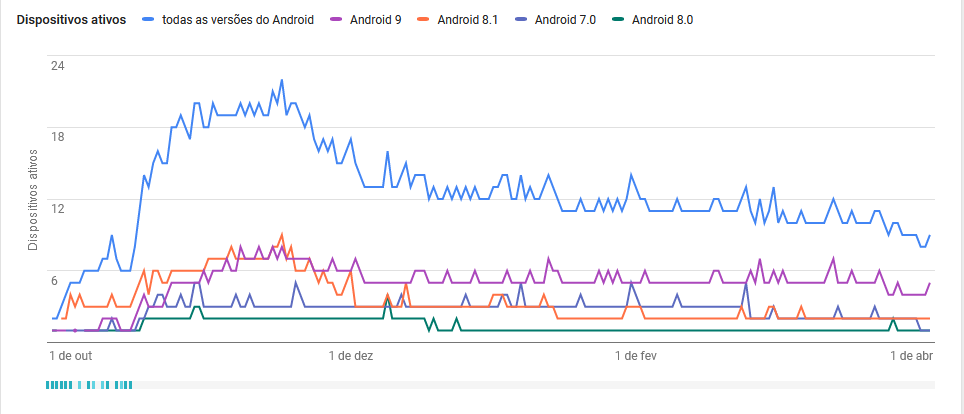
\includegraphics[scale=0.25]{Imagens/taxa_desocupacao.png}
\fonte{\citeonline{ibge_instituto_brasileiro_de_geografia_e_estatistica_pesquisa_2019}}
\label{figura_2}
\end{figure}


Com as universidades e institutos de ensino superior sendo reconhecidamente contextualizados como promotores da inovação no Brasil, país que configura o 13.º lugar entre os maiores produtores de publicações de pesquisa (\textit{papers}) e inovação a nível mundial, \citeonline{clarivate_analytics_web_of_research_2017}. 
O novo paradigma educacional, portanto, situa as instituições de ensino superior no campo da promoção do empreendedorismo direcional e sistemático, assim como o comportamento empreendedor, educação empreendedora disciplinada mostra-se eficaz no tocante ao surgimento das inovações, direcionadas e a promoção da identidade empreendedora para novos negócios, \cite{jain_academics_2009} já que a universidade vem a ser um local privilegiado do saber, da liberdade acadêmica e da experimentação científica tem o poder de ‘oficializar’ o empreendedorismo como um conteúdo de conhecimento é uma ferramenta capaz de gerar inovações \cite{dolabela_oficina_2008}. 

Já que o desenvolvimento do interesse ao empreendedorismo envolve diversos conteúdos de aprendizado, é necessário organizar as metodologias e suas aplicações pedagógicas \cite{rocha_avaliacao_2014}. O mesmo autor elencou os Principais Métodos, Técnicas e Recursos Pedagógicos no Ensino do Empreendedorismo. 


\begin{center}
\renewcommand\LTcaptype{quadro}
\begin{longtable}{p{3.5cm}p{11.0cm}}

\caption[\textbf{Principais  Métodos, Técnicas e Recursos Pedagógicos no Ensino de Empreendedorismo}]{\textbf{Principais  Métodos, Técnicas e Recursos Pedagógicos no Ensino de Empreendedorismo}} \label{tabela_2} \\


\hline \multicolumn{1}{p{3.5cm}}{\textbf{Métodos, Técnicas e Recursos}} & \multicolumn{1}{c}{\textbf{Aplicações}}\\ \hline 

\endfirsthead


\multicolumn{2}{c}%

{{\bfseries \quadroname \ \thequadro{} -\ \textbf{Continuação}}}\\

\hline \multicolumn{1}{p{3.5cm}}{\textbf{Métodos, Técnicas e Recursos}} & \multicolumn{1}{c}{\textbf{Aplicações}}  \\ \hline 

\endhead

\hline \multicolumn{2}{r}{{\textbf{Continua}}} \\ \hline

\endfoot
\hline \multicolumn{2}{r}{{\textbf{Continua}}} \\ \hline

\endfoot
\hline \multicolumn{2}{r}{{\textbf{Conclusão}}} \\ \hline
\hline \hline

\endlastfoot

Aulas expositivas & Transferir conhecimentos sobre o Empreendedorismo, as características pessoais do empreendedor, os processos de inovação, fontes de recursos, financiamentos e aspectos legais de pequenas empresas.  \\

Visitas e contatos com empresas & Estimular o \textit{network} e incitar o estudante a sair dos limites da IES para entender o funcionamento de mercado na vida real. Desenvolver visão de mercado.  \\

Plano de negócios & Desenvolver as habilidades de planejamento, estratégia, marketing, contabilidade, recursos humanos, comercialização. Desenvolver a habilidade de avaliação do novo negócio, analisando o impacto da inovação
no novo produto ou serviço. Construir habilidade de avaliar e dimensionar riscos do negócio pretendido. \\ 

Estudos de situações problemas & Construção da habilidade de pensamento crítico e de avaliação de cenários e
negócios. Desenvolver a habilidade de interpretação e definição de contextos associados ao Empreendedorismo. \\ 

Trabalhos teóricos em grupo & Construção da habilidade de aprender coletivamente. Desenvolver a
habilidade de pesquisar, dialogar, integrar e construir conhecimentos,
buscar soluções e emitir juízos de valor na realização do documento escrito. \\ 

Trabalhos práticos em grupo & Construção da habilidade de atuar em equipe. Desenvolver a habilidade de planejar, dividir e executar tarefas em grupo, de passar e receber críticas construtivas. Ampliar a integração entre o saber e o fazer.  \\ 

Grupos de discussão & Desenvolver a habilidade de testar novas ideias. Desenvolver a capacidade de avaliar mudanças e prospectá-las como fonte de oportunidades. \\ 
 
\textit{Brainstorming}  & Construção da habilidade de concepção de ideias, prospecção de
oportunidades, reconhecendo-as como oportunidades empreendedoras. \\ 


Seminários e palestras com empreendedores & Transferir conhecimentos das experiências vividas por empreendedores
desde a percepção e criação do produto, abertura do negócio, sucessos e
fracassos ocorridos na trajetória empreendedora. \\ 

Criação de empresa & Transpor as informações do plano de negócios e estruturar os contextos necessários para a formalização. Compreender várias etapas da evolução da empresa. Desenvolver a habilidade de organização e planejamento operacional. \\ 

Aplicação de provas dissertativas & Testar os conhecimentos teóricos dos estudantes e sua habilidade de
comunicação escrita. \\ 

Atendimento individualizado & Desenvolver a habilidade de comunicação, interpretação, iniciativa e
resolubilidade. Aproximar o estudante do cotidiano real vivido nos pequenos negócios. \\ 

Trabalhos teóricos individuais & Construção da habilidade de concepção de conhecimento individualizado,
estimulando a autoaprendizagem. Induzir o processo de autoaprendizagem. \\ 

Trabalhos práticos individuais & Construção da habilidade da aplicação dos conhecimentos teóricos
individuais, estimulando a autoaprendizagem. Estimular a capacidade
laboral e de auto realização. \\ 

Criação de produto & Desenvolver habilidade de criatividade, persistência, inovação e senso de
avaliação. \\ 

Filmes e vídeos & Desenvolver a habilidade do pensamento crítico e analítico, associando o
contexto assistido com o conhecimento teórico. Estimular a discussão em grupo e o debate de ideias. \\ 

Jogos de empresas e simulações & Desenvolver a habilidade de criar estratégias de negócios, solucionar
problemas, trabalhar e tomar decisões sob pressão. Aprender pelos próprios erros. Desenvolver tolerância ao risco, pensamento analítico, comunicação intra e intergrupais. \\ 

Sugestão de leituras & Prover ao estudante teoria e conceitos sobre o Empreendedorismo. Aumentar a conscientização do ato empreendedor. \\ 
Incubadoras & Proporcionar ao estudante espaço de motivação e criação da nova empresa, desenvolvendo múltiplas competências, tais como habilidades de liderança, organizacionais, tomada de decisão e compreender as etapas do ciclo de vida das empresas. Estimular o fortalecimento da network com financiadores, fornecedores e clientes. \\

Competição de planos de negócios & Desenvolver habilidades de comunicação, persuasão e estratégia.
Desenvolver capacidade de observação, percepção e aplicação de melhorias no padrão de qualidade dos planos apresentados. Estimular a abertura de empresas mediante os planos vencedores. \\ 

\end{longtable}
\fonte{\cite{rocha_avaliacao_2014}}
\renewcommand\LTcaptype{quadro}
\end{center}



Os centros de ensino devem contribuir para o desenvolvimento da “cultura empreendedora” por meio da “educação empreendedora” \cite{tscha_empreendendo_2014}, que incentive tanto Docentes quanto aos Discentes, deve incentivar “o despertarem dentro de si o espírito empreendedor e a explorar o espaço potencial para o empreendedorismo, transformando realidades por meio dos empreendimentos que podem desenvolver economicamente e socialmente um país e uma sociedade” \cite{tscha_empreendendo_2014}. Uma vez que, a cultura empreendedora depende diversos fatores influenciáveis ao longo do aprendizado e vida. \cite{dornelas_empreendedorismo:_2005} explica que  empreender segue fluxo um definido que depende de fatores determinantes durante a construção correta e satisfatória da cultura empreendedora. Alguns fatores estão descritos na figura \ref{figura_2}.

\begin{figure}[!htb]
\centering
\caption{\textbf{Fatores que influenciam o aprendizado do comportamento empreendedor:}}
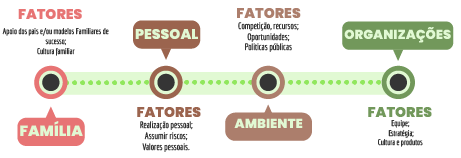
\includegraphics[scale=0.8]{Imagens/esquema_influencias_empreendedorismo.png}
\fonte{Adaptado de \cite{dornelas_empreendedorismo:_2005}}
\label{figura_2}
\end{figure}


Empreendedorismo acadêmico  apresenta-se também como uma potencial ferramenta para difusão e transferência de inovação e pesquisa por acadêmicos oriundos de laboratórios ou, departamentos onde a tecnologia se originou, \cite{guo_what_2019, abreu_nature_2013}, ou mesmo a busca de oportunidades e iniciativa utilizando os meios existentes no ambiente acadêmico. Os conteúdos necessários ao efetivo ensino do empreendedorismo vão além da oferta de apenas uma disciplina, é preciso que a instituição de ensino, a partir de novas práticas pedagógicas, transforme-se em também em uma instituição empreendedora \cite{campelli_empreendedorismo_2011}, que visualize a potencialidade da educação e promoção do comportamento empreendedor ao aluno com vistas a resolutividade de problemas \cite{degen_o_1989} e despertar da criatividade.

Diante da necessidade de solidificar o ensino empreendedor, que a \textit{Commission Enterprise and Industry Directorate-General} \cite{european_commission_best_2008} estruturou a educação empreendedora direcionada ao ensino superior em três objetivos, representados no modelo esquemático que pode ser visto na Figura \ref{figura_3}, em que se explica às três bases que estruturam os objetivos do ensino do Empreendedorismo no meio acadêmico. 

\begin{figure}[!htb]
\centering
\caption{\textbf{Pilares dos objetivos do ensino ao empreendedorismo.}}
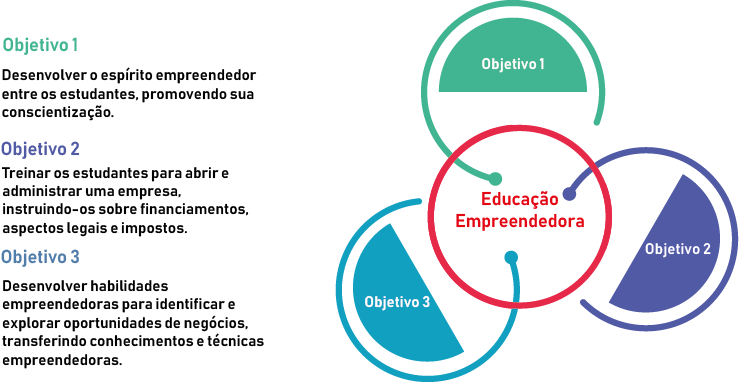
\includegraphics[scale=0.8]{Imagens/figura2.png}
\fonte{Adaptado de \cite{european_commission_best_2008}}
\label{figura_3}
\end{figure}


Como visto, ensino do empreendedorismo perpassa por diversas vertentes, porém, visando a associação de tais conteúdos aos técnicos científicos de forma interdisciplinar, e explorado neste trabalho a proposta de educação empreendedora que tem como base a Aprendizagem Baseada em Problemas (ABPR), a Aprendizagem Baseada em Projetos (ABP) \cite{bender_aprendizagem_2015} tendo como passos para elaboração dos conteúdos para o desenvolvimento de um empreendimento bem-sucedido os passos de \cite{aulet_empreendedorismo_2019} no livro: Empreendedorismo Disciplinado. 
Segundo \cite{bender_aprendizagem_2015} a ABP tem como objetivo o desenvolvimento do autoconhecimento com ênfase na perseverança, na imaginação, na criatividade, na inovação, para resolubilidade de problemas reais, sendo um importante o conteúdo que se aprende a fazer, mas, sobretudo, o que aprendido \cite{souza_disseminacao_2001}, de forma que a união de tais conhecimentos se some a um melhor desenvolvimento aos profissionais graduados que irão ao mercado de trabalho ou ao mundo dos negócios. Já que conhecimento científico promovido de forma interdisciplinar na graduação, além de repassar os conhecimentos técnicos, promove  uma considerável contribuição para se desenvolver o raciocínio independente, criativo e inovador buscamos nesta pesquisa uma abordagem que possa explorar todos os conteúdos de uma metodologia disciplinada e estruturada.


\section{Propriedade Intelectual no meio rural}

Toda criação advinda do intelecto humano, tais como música, produto, processo, nova cultivar, desenhos, artigos científicos, trabalhos literários ou artísticos constituem um ativo, bem ou direito \cite{costa_interseccao_2011}. Tais ativos sendo eles registrados ou não estão ligados diretamente ao seu autor/inventor sendo a propriedade  intelectual. Este direito vai muito além da inovação em si \cite{wipo_tratado_1970}, mas a relação entre o seu autor/inventor e sua respectiva criação intelectual. 


O conceito de Propriedade Intelectual é amplo e difere de país a país, em suma pode ser entendido como, à área do Direito que, garante a inventores ou responsáveis por qualquer produção do intelecto, seja nos domínios industrias, científicos, literários ou artísticos, o direito de obter, por um determinado período de tempo, recompensa pela própria criação \cite{aspi_aspi_2019}, é amparo legal e necessário para garantir que os investimentos em pesquisa e desenvolvimento retornem ao inventor, provocando um processo cíclico positivo, em que maiores investimentos em P&D seriam promovidos diante da concessão do monopólio temporário de exploração do invento \cite{lima_sauglobal_2017}. No Brasil a PI é composta por três grandes áreas: Propriedade Industrial, Direito do Autor e Suis generis, demais ramificações podem ser vistas na figura \ref{figura_4}.


\begin{figure}[h!]
\centering
\caption{\textbf{Modalidades da propriedade intelectual no Brasil}}
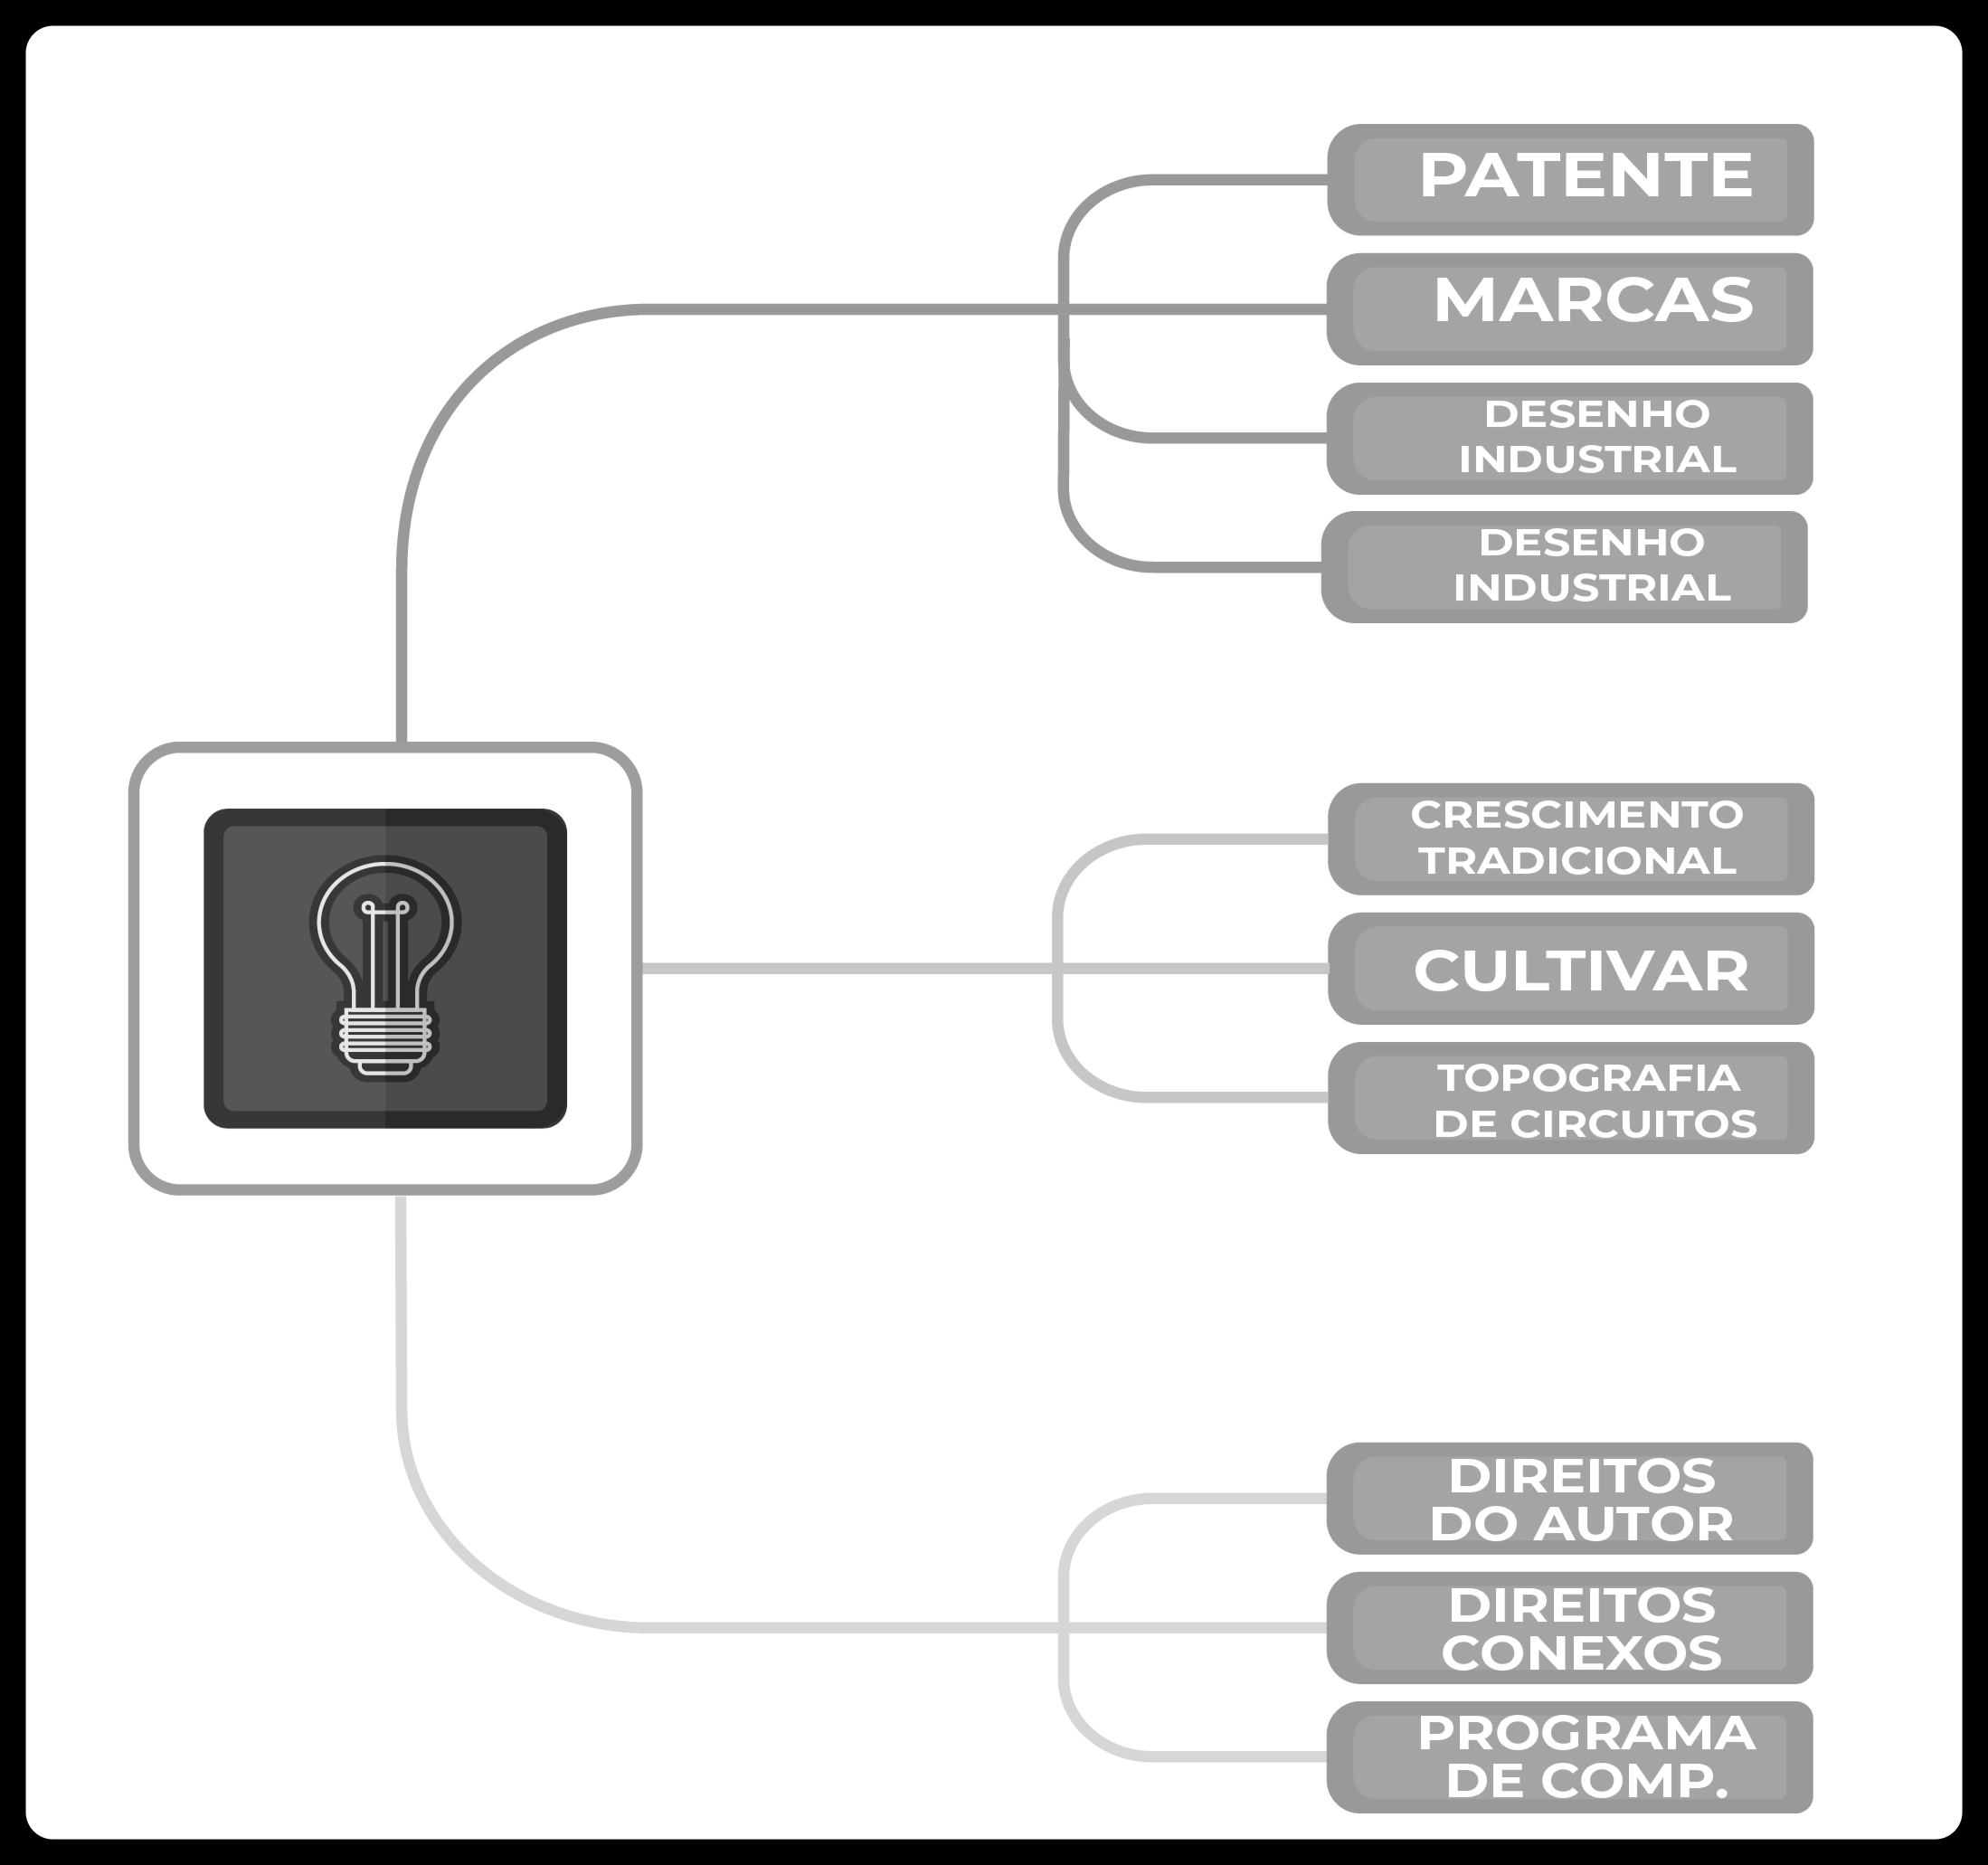
\includegraphics[scale=0.75]{Imagens/propriedade_intelectual.png}
\fonte{Adaptado de \cite{inpi_manual_2017}}
\label{figura_4}
\end{figure}


Aliadas  às  ações  para  o  desenvolvimento  de  inovações, o inventor ou autor deve ter certa atenção as Propriedades Intelectuais que tangem seu produto, ou processo.  Sendo assim, é visível que há uma grande afinidade entre estes dois temas, principalmente os direitos que cabe ao meio industrial e do autor ligados a software. 

A crescente interação comercial,  financeira  e  tecnológica  entre  a  economia  e  seus  agentes  exigem  padrões  modernos  de  proteção  para  a  PI,  uma  vez  que  os  direitos sobre os nomes empresariais, tecnologias, \textit{designs}, marcas, entre outros, representam valiosos ativos das empresas e profissionais autores/inventores \cite{sherwood_propriedade_1992}. 


Diante de tais mudanças sobre o cenário do desenvolvimento tecnológico e das Propriedades Intelectuais (PI) inúmeras questões sobre o papel que os sistemas de registro e divulgação para PI desempenham no desenvolvimento e o incentivo à inovação \cite{segala_os_2016}. Os países que apresentam uma economia mais forte, dispõe de um sistema de proteção de propriedade mais robusto e confiável, concomitantemente, uma maior quantidade de registros e depósitos das mais variadas finalidades \cite{mueller_universidades_2014}.




\chapter{METODOLOGIA}

%Metodologia da bibliografia
\section{Metodologia usada no Levantamento Bibliográfico}


Para atingir os objetivos que orientam este estudo, os procedimentos metodológicos foram planejados tendo como base programas educacionais que visam a promoção do empreendedorismo e comportamento empreendedor na condução dos cursos de graduação, em instituições de ensino públicas e particulares, como também Startups de natureza educacional. A metodologia de pesquisa utilizada encontra-se esquematizada na Figura \ref{figura_29}, os artigos foram exportados para o software StArt \cite{lapes_start_2016}. A ferramenta StArt foi desenvolvida para apoiar todo processo de Revisão Bibliográfica. Por meio de uma árvore hierárquica, categorizando os artigos em proximidade e níveis de aderência as palavras-chave \cite{hernandes_avaliacao_2010}. 

\begin{figure}[!htb]
\centering
\caption{\textbf{Planejamento da pesquisa e construção do portfólio de artigos}}
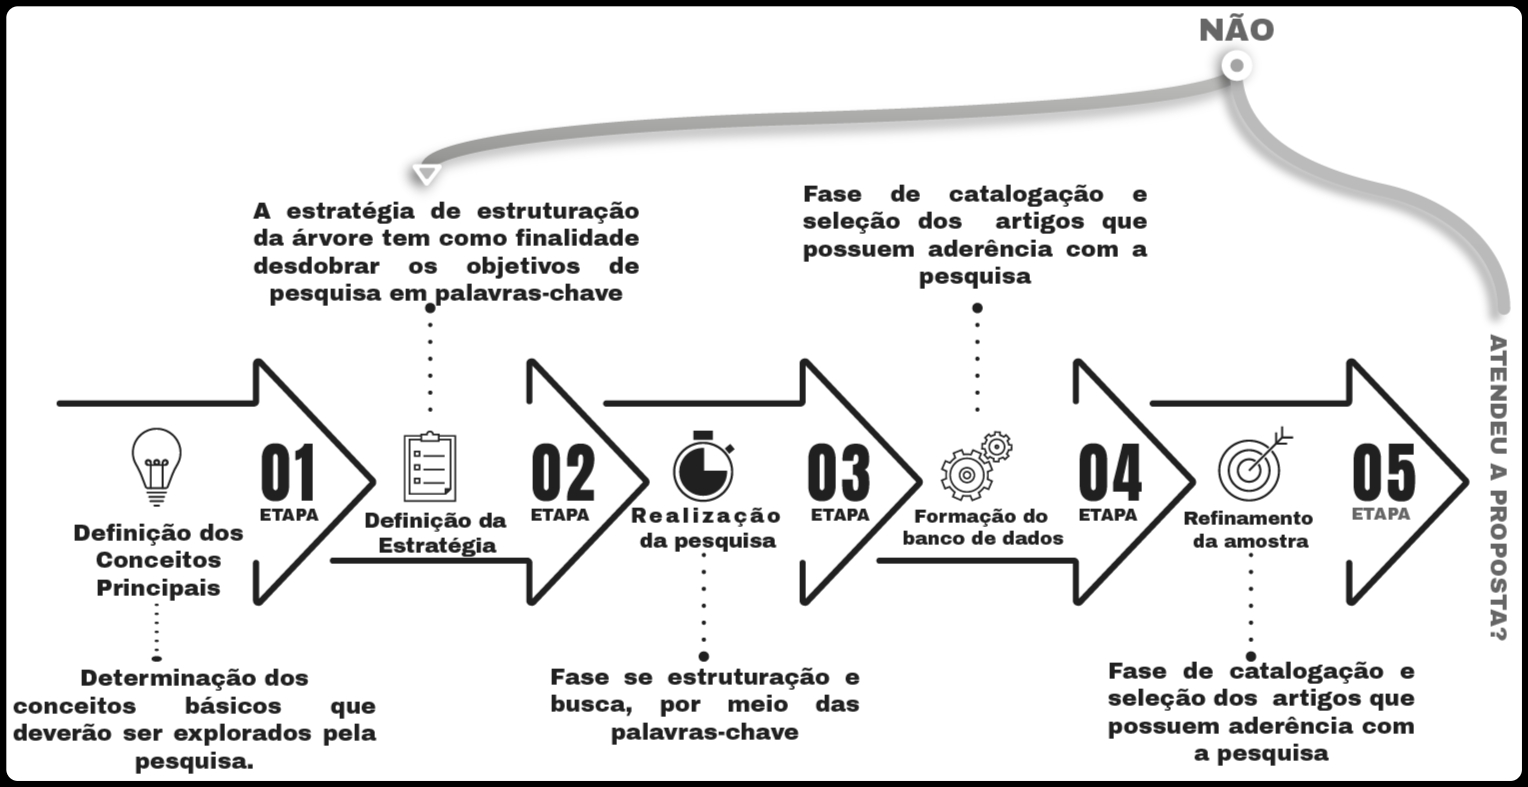
\includegraphics[scale=0.5]{Imagens/fases_pesquisa_bibliografica.png}
\fonte{Adaptado de \citeonline{hernandes_avaliacao_2010}}
\label{figura_29}
\end{figure}






\section{Programa Empreenda AGRO Sustentável: considerações metodológicas}


As atividades serão desenvolvidas em quatro encontros \textit{(workshops)}, que constam metodologias ativas, oficinas, palestras, e ferramentas tecnológicas visando à sinergia entre as estratégias de inovação no uso de tecnologias educacionais e os objetivos da proposta, com vistas a promover aprendizagem significativa e colaborativa. Todas as etapas do projeto de pesquisa serão executadas utilizando a metodologias ativas, objetivando o aprendizado do uso das ferramentas de gestão e desenvolvimento de negócios.
Durante os módulos do projeto (Workshops), os participantes testarão de seus projetos para que novas requisições sejam realizadas e/ou que erros nos planejamentos sejam encontrados e, consequentemente, debatidos e mitigados, utilizando para isso os métodos de modelagem de negócio \textit{(Lean Canvas e Business Model Canvas)}. Depois que todas as Sprints (atividades dos três Workshops) forem finalizadas, ou seja, que todos os módulos forem trabalhados, será iniciado um ciclo de Apresentações e desenvolvimento da habilidade de apresentação e demonstração dos produtos com apresentações (\textit{Pitch}). Destaca-se, ainda, que as inovações passiveis de registro intelectual apresentadas nesta pesquisa serão incentivadas a registro e documentação dos direitos.



\section{Planejamento Pedagógico}

O Programa Empreenda Agro Sustentável traz a proposta do trabalho ao ensino do empreendedorismo de forma multidimensional, multidisciplinar e disciplinado. Tal programa utilizou-se de Workshops particionados em temas que permitem a compreensão global do empreendedorismo, enquanto admite o ser humano como um ser multidimensional e culturalmente contextualizado no desenvolvimento de um negócio inovador. 

A proposta do programa é combinar oficinas que visam o desenvolvimento das características negociais e seus planos com palestras ministradas por profissionais de alto conhecimento nas áreas específicas de um negócio escalável. Com a aprendizagem baseada em equipes \textit{(team-based learning)} o programa delimitou inicialmente a inscrição dos participantes somente em equipes pré-estabelecidas, de modo a ter como iniciativa, maiores afinidades durante o desenvolvimento dos trabalhos. 


Com a finalidade de propor uma melhor mentoria no desenvolvimento dos objetivos propostos, o programa será desenvolvido em quatro encontros (Workshops) (Figura \ref{figura_17}), que abordarão temas pertentes ao empreendedorismo e o comportamento empreendedor, a saber:

\begin{itemize}

\item {1º Workshop \textbf{INSIGHT E DESPERTAR}: O que é startups, empreendedorismo, comportamento empreendedor e cultura empreendedora, problemas (segmentação do mercado), segundo os Objetivos do Desenvolvimento Sustentável (ODS), Modelagem do negócio e Criatividade;}
\item {2º Workshop \textbf{IDEAÇÃO}: A busca de oportunidades como característica empreendedora, construção do \textit{Lean Canvas}, mapa de empatia, validação da proposta de valor, economia colaborativa e \textit{coworking};}

\item {3º Workshop: \textbf{MAKEATHON}: Prototipagem para o MCVP, O que você pode fazer por seu cliente e como o cliente adquire seu produto?;}

\item {4º Workshop \textbf{DEMODAY}: Destaca-se que o mecanismo de pesquisa que será utilizado neste experimento foi composto por Cinco blocos de questões de múltipla escolha baseadas principalmente em escalas de cinco ou sete possibilidades.}
\end{itemize}

\begin{figure}[!htb]
\centering
\caption{\textbf{Jornada Empreenda Agro Sustentável}}
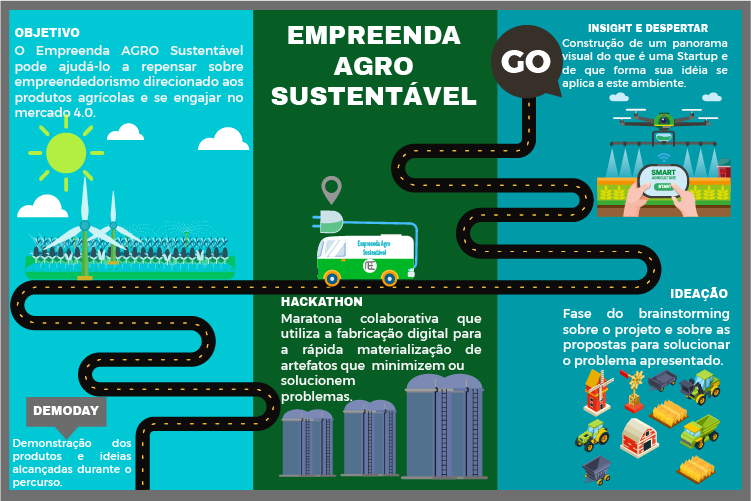
\includegraphics[scale=0.3]{Imagens/jornada.png}
\fonte{Próprio Autor}
\label{figura_17}
\end{figure}





\subsection{1º Workshop}

Buscando um engajamento maior dos participantes foram
aplicadas cinco estratégias/dinâmicas: Apresentação das ideias propostas inicialmente; Círculo Dourado;
Quem sou eu no Universo?; Descoberta do cliente usuário e o  desenvolvimento da proposta de valor Figura \ref{figura_30}.

\begin{figure}[!h]
\centering
\caption{\textbf{1º Workshop Empreenda Agro Sustentável}}
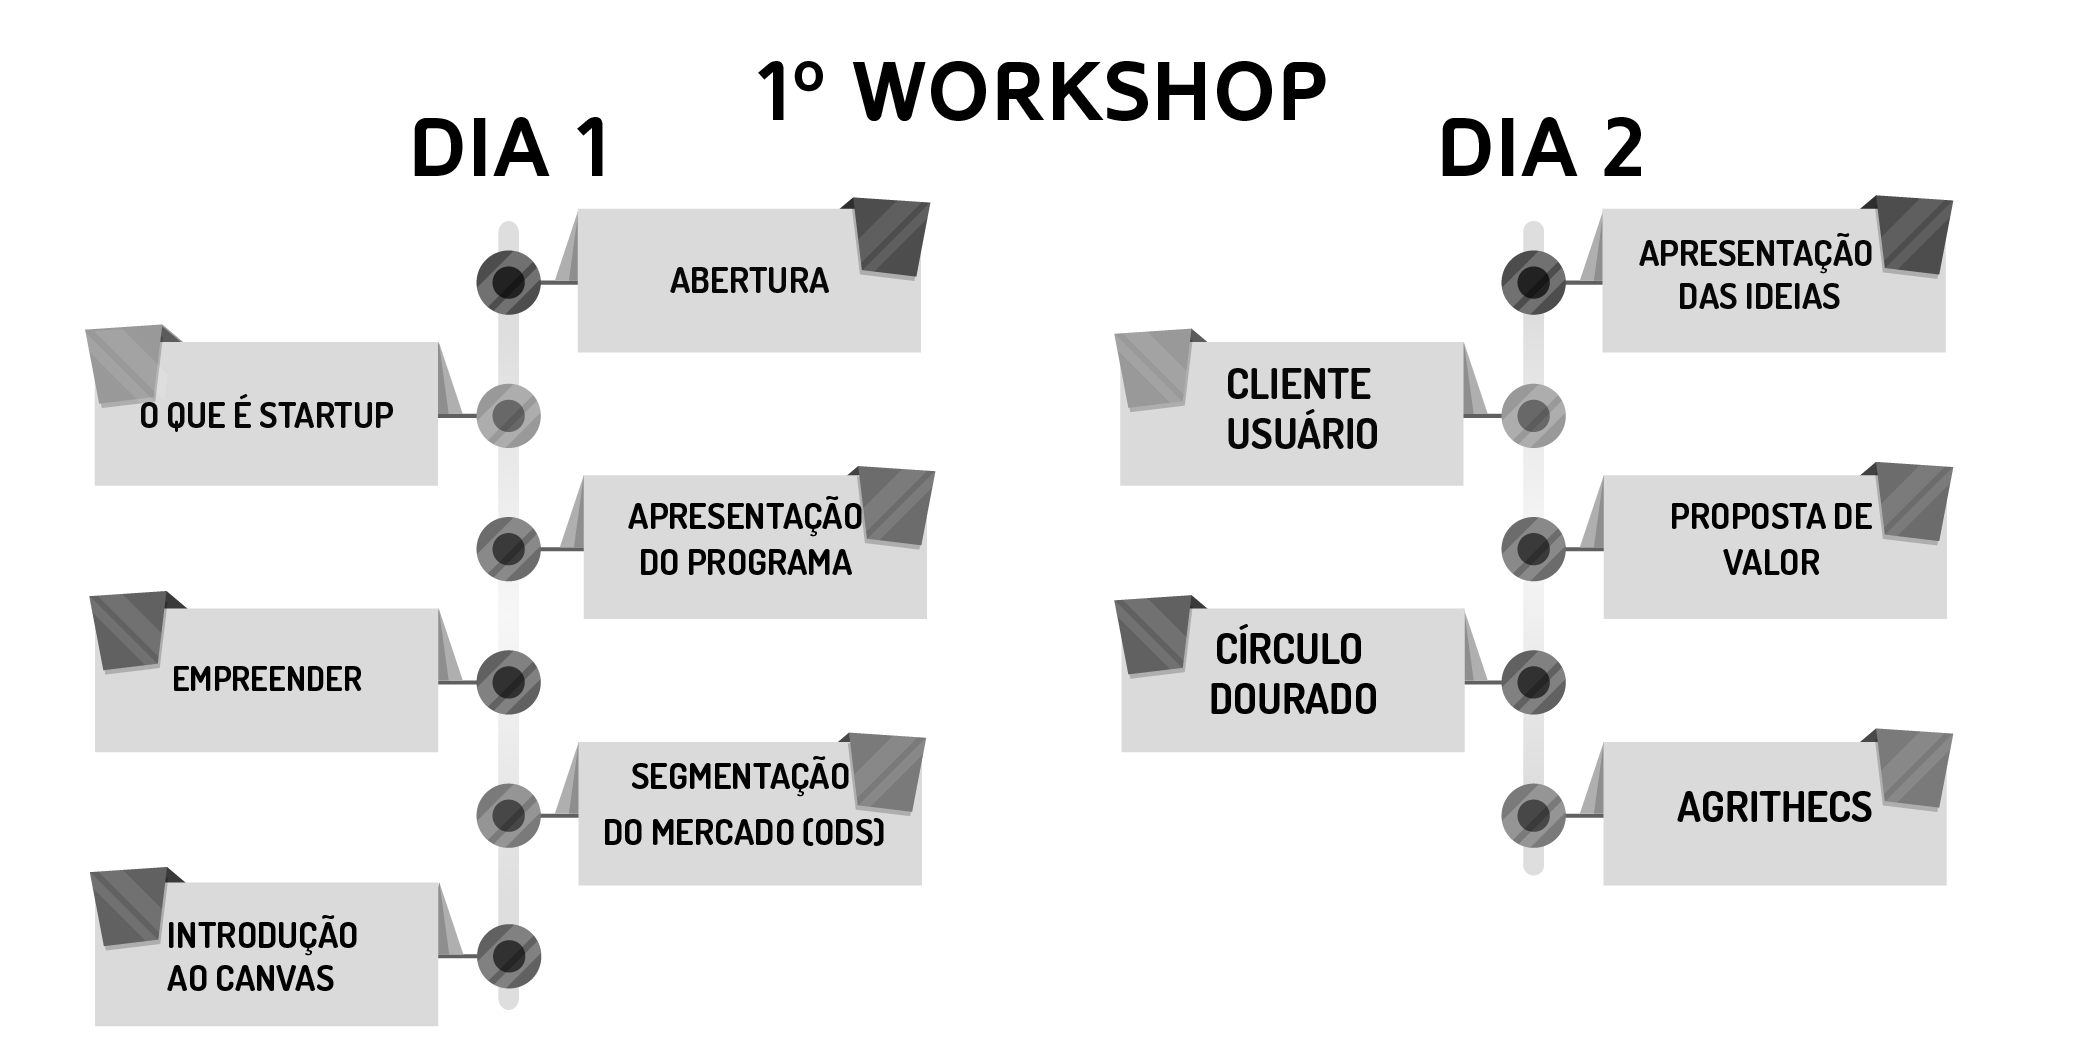
\includegraphics[scale=0.3]{Imagens/workshop-01.png}
\fonte{Próprio Autor}
\label{figura_30}
\end{figure}
%\newpage

A dinâmica \textbf{"Apresentação das ideias propostas"}\ visa a construção de um panorama visual de todos os insights, inscritas no programa, como também as temáticas mais buscadas pelos alunos. As atividades de Expressão Oral (EO) oportunizam aos estudantes a apropriação de recursos linguísticos e interativos inerentes às práticas orais e considerando que a EO pode ser uma eficaz ferramenta para a ensinagem de conteúdos conceituais, procedimentais e atitudinais em contato social \cite{baltar_genero_2010}.

A atividade proposta, considera que a expressão oral mesmo que incipiente proporcionara aos alunos e todo o grupo o exercício da criticidade, abordar e levantar seus pontos de vista e seus interesses na participação do programa pode executar a sua verve crítica, defender seus pontos de vista enquanto possibilita o aprimoramento das atitudes discursivas da ordem do expor e do argumentar, já que o estudante torna público suas expectativas e se compromete informalmente a comunidade de desenvolver suas propostas. 

Já a segunda dinâmica \textbf{Golden Circle} desenvolvido por \citeonline{sinek_golden_2015} tem por objetivo: criar ou desenvolver o valor de um novo produto, ideia ou negócio, tal dinâmica é pautada em três pilares: O quê, Como e Porquê. O Círculo Dourado e formado por três círculos de diferentes tamanhos que se completam. Ao centro está o \textbf{Porquê}, tal círculo objetiva a expressão do real propósito do negócio pensado pelo grupo. Este Refere-se ao conjunto de iniciativas e compromissos pensados para escalar e promover aos usuários e clientes o valor que a Startup realmente acredita. Resumidamente é o que a empresa de fato acredita ser o  diferencial perante a concorrência e ao mercado atual, este é o ponto de partida, principal círculo da dinâmica. 


\begin{figure}[!h]
\centering
\caption{\textbf{Golden Circle}}
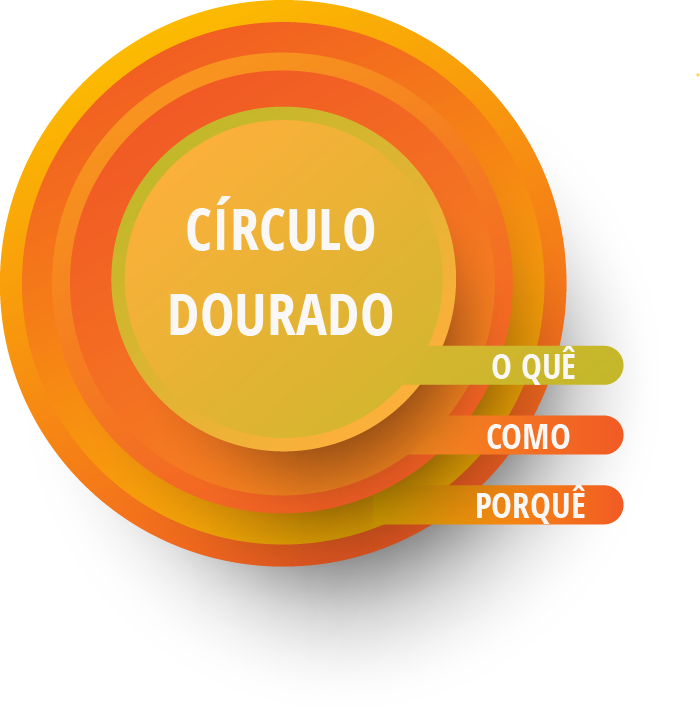
\includegraphics[scale=0.3]{Imagens/circulo_dourado.png}
\fonte{Adaptado de: \cite{sinek_golden_2015}.}
\label{figura_5}
\end{figure}
\newpage

\subsection{2º Workshop}

Tendo a perspectiva macro do que venha a ser inovação e meios de negócios, o segundo encontro trará a proposta de descoberta de oportunidades e desenvolvimento do insight, por meio da busca de oportunidades e mineração de inovações Figura \ref{figura_31}.


\begin{figure}[!h]
\centering
\caption{\textbf{2º workshop Empreenda Agro Sustentável}}
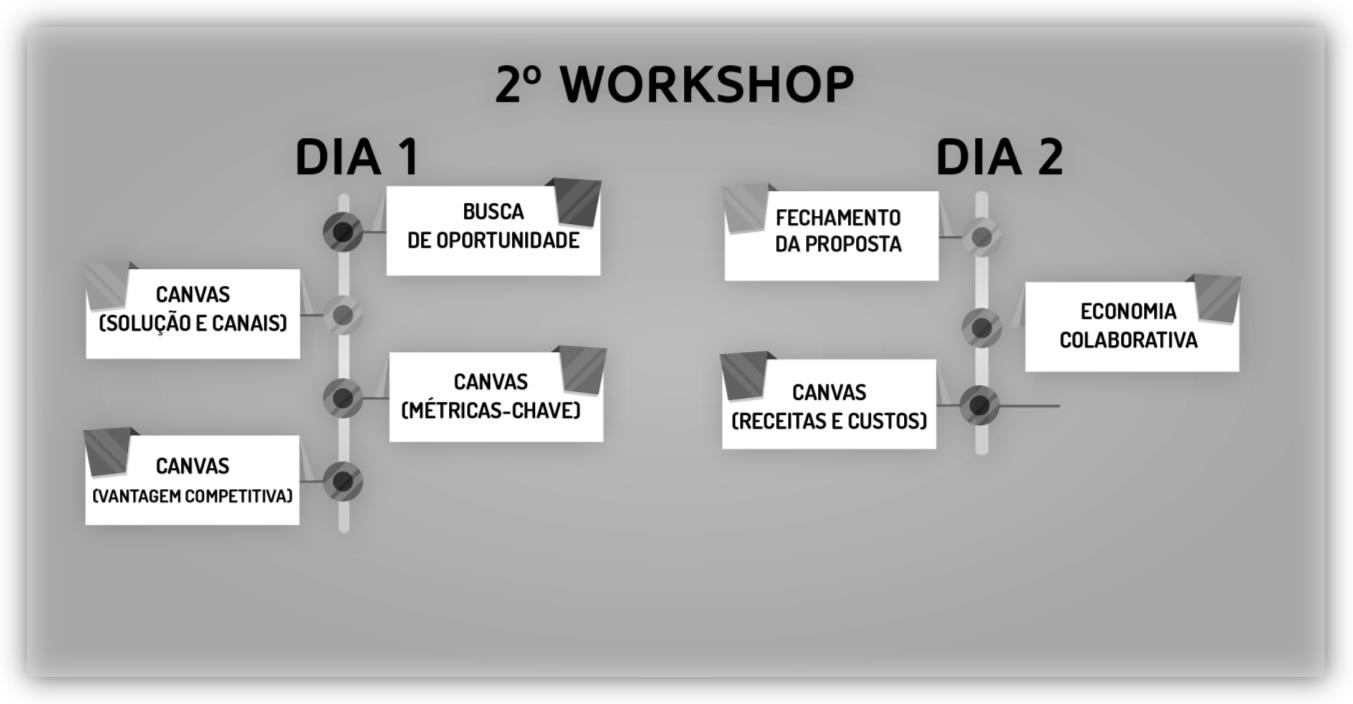
\includegraphics[scale=0.3]{Imagens/workshop-02.png}
\fonte{Próprio Autor.}
\label{figura_31}
\end{figure}

Será construído o Mapa de empatia de modo a compreender os desejos e necessidades dos clientes e usuários até mesmo seu estado emocional, que influenciará os seus anseios a aquisição de produtos e serviços. Esta necessidade de entender e assimilar as necessidades dos usuários é prioridade no atendimento das expectativas e necessidades dos usuários, é um ponto fundamental para que as unidades de informação trabalhem orientadas à qualidade e com possibilidade de incorporação de serviços inovadores \cite{valdrich_mapa_2018}. O mapa de empatia é uma ferramenta visual para conduzir esta descoberta, ele é comporto por 6 (seis) reflexões diferentes sobre o cliente, são elas: \textbf{as dores}, \textbf{os ganhos},\textbf{o que ele escuta}, \textbf{o que ele vê}, \textbf{o que ele pensa e sente} e  \textbf{o que ele faz}, é possível entender o mapa de empatia por meio da figura \ref{figura_6}. 


\begin{figure}[h!]
\centering
\caption{\textbf{Exemplo do Mapa de empatia}}
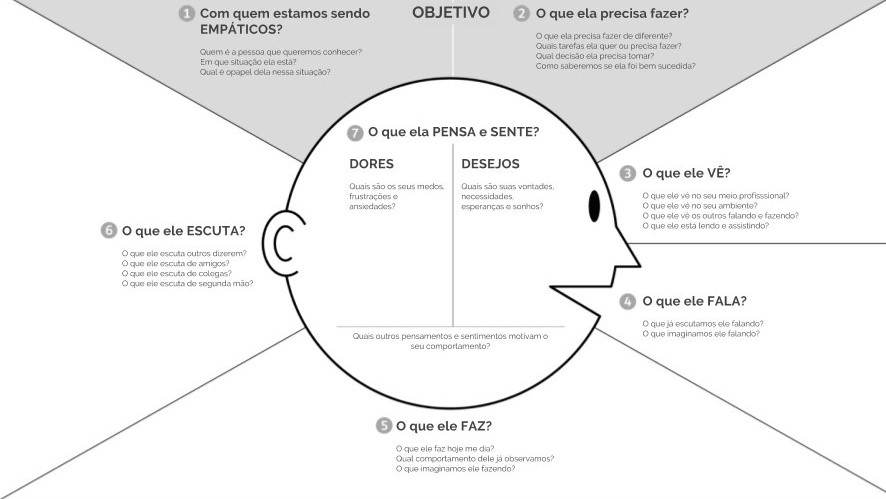
\includegraphics[scale=0.4]{Imagens/mapa_empatia.jpg}
\fonte{\cite{osterwalder_value_2019}.}
\label{figura_6}
\end{figure}


Após o desenvolvimento da ideia da Startup por meio do mapa de empatia, é esperado que o participante tenha uma visão holística do que deseja produzir como negócio, assim para que seja visualizado as possibilidades e estruturas do negócio será trabalhado o quadro ferramenta Lean Canvas proposto por Ash Maurya, tendo como base para o desenvolvimento o \textit{Business Model Canvas} (BMC) entre outros materiais. Ele adaptou 4 quadros do BMC, buscando trabalhar aspectos de maior risco na criação de Startups \cite{maurya_running_2012}. Ele é ideal para o quando o negócio está no começo ou ainda não deu início às atividades e que ainda não fez testes sobre suas estruturas comerciais. Essa é a hora de analisar de maneira mais aprofundada os problemas que o mercado apresenta e estruturar de uma forma melhor a solução oferecida pela startup, encontrando aí o melhor resultado nessa equação \cite{sebrae_aprenda_2019}. O quadro é comporto pelos seguintes campos: \textbf{1.\textsuperscript{o} Problema, 2.\textsuperscript{o} Segmentos de Clientes, 3.\textsuperscript{o} Proposta Única de valor, 4.\textsuperscript{o} Solução, 5.\textsuperscript{o} Canais, 6.\textsuperscript{o} Fontes de Receitas e 7.\textsuperscript{o} Estrutura de Custos}. 

O problema deve ser as dificuldades que a startup deve resolver por seus usuários o segmento de Clientes: deve prever quais os clientes e usuários da sua 'startup'? De que forma eles podem ser segmentados? Na que torna o seu produto diferente e merecedor do dinheiro dos clientes, o que de fato a startup tem a oferecer ao cliente/usuário. No campo (Solução) o aluno deve explicar o menor conjunto de funcionalidades de seu produto, de que forma ele vai entregar a proposta de valor anteriormente pensada. Ao chegar nas métricas chaves eles deverão planejar como será a geração de capital deste negócio ou de que forma reterão seus clientes/usuários, no campo (Canais), será descrito uma lista de meios de marketing e captação de cliente. Para a estrutura de custos, os participantes descreverão todos os gastos sendo custos fixos e variáveis de seu negócio, já para o Fluxo de Receita ele identificará qual o tipo de modelo de receita – assinatura, anúncios, \textit{freemium}, e determine as premissas para indicadores como \textit{Life time value}, etc. Por fim, na vantagem competitiva deve ser explicado o algo que não pode ser comprado ou copiado, deve ser de fato a inovação de seu negócio, \cite{maurya_running_2012, sebrae_aprenda_2019}. É recomendável a construção do quadro seguindo esta sequência, na figura \ref{figura_7} é possível visualizar o quadro que será utilizado durante o programa. 



\begin{figure}[h!]
\centering
\caption{\textbf{Quadro Lean Canvas adaptado para o Programa Empreenda Agro Sustentável}}
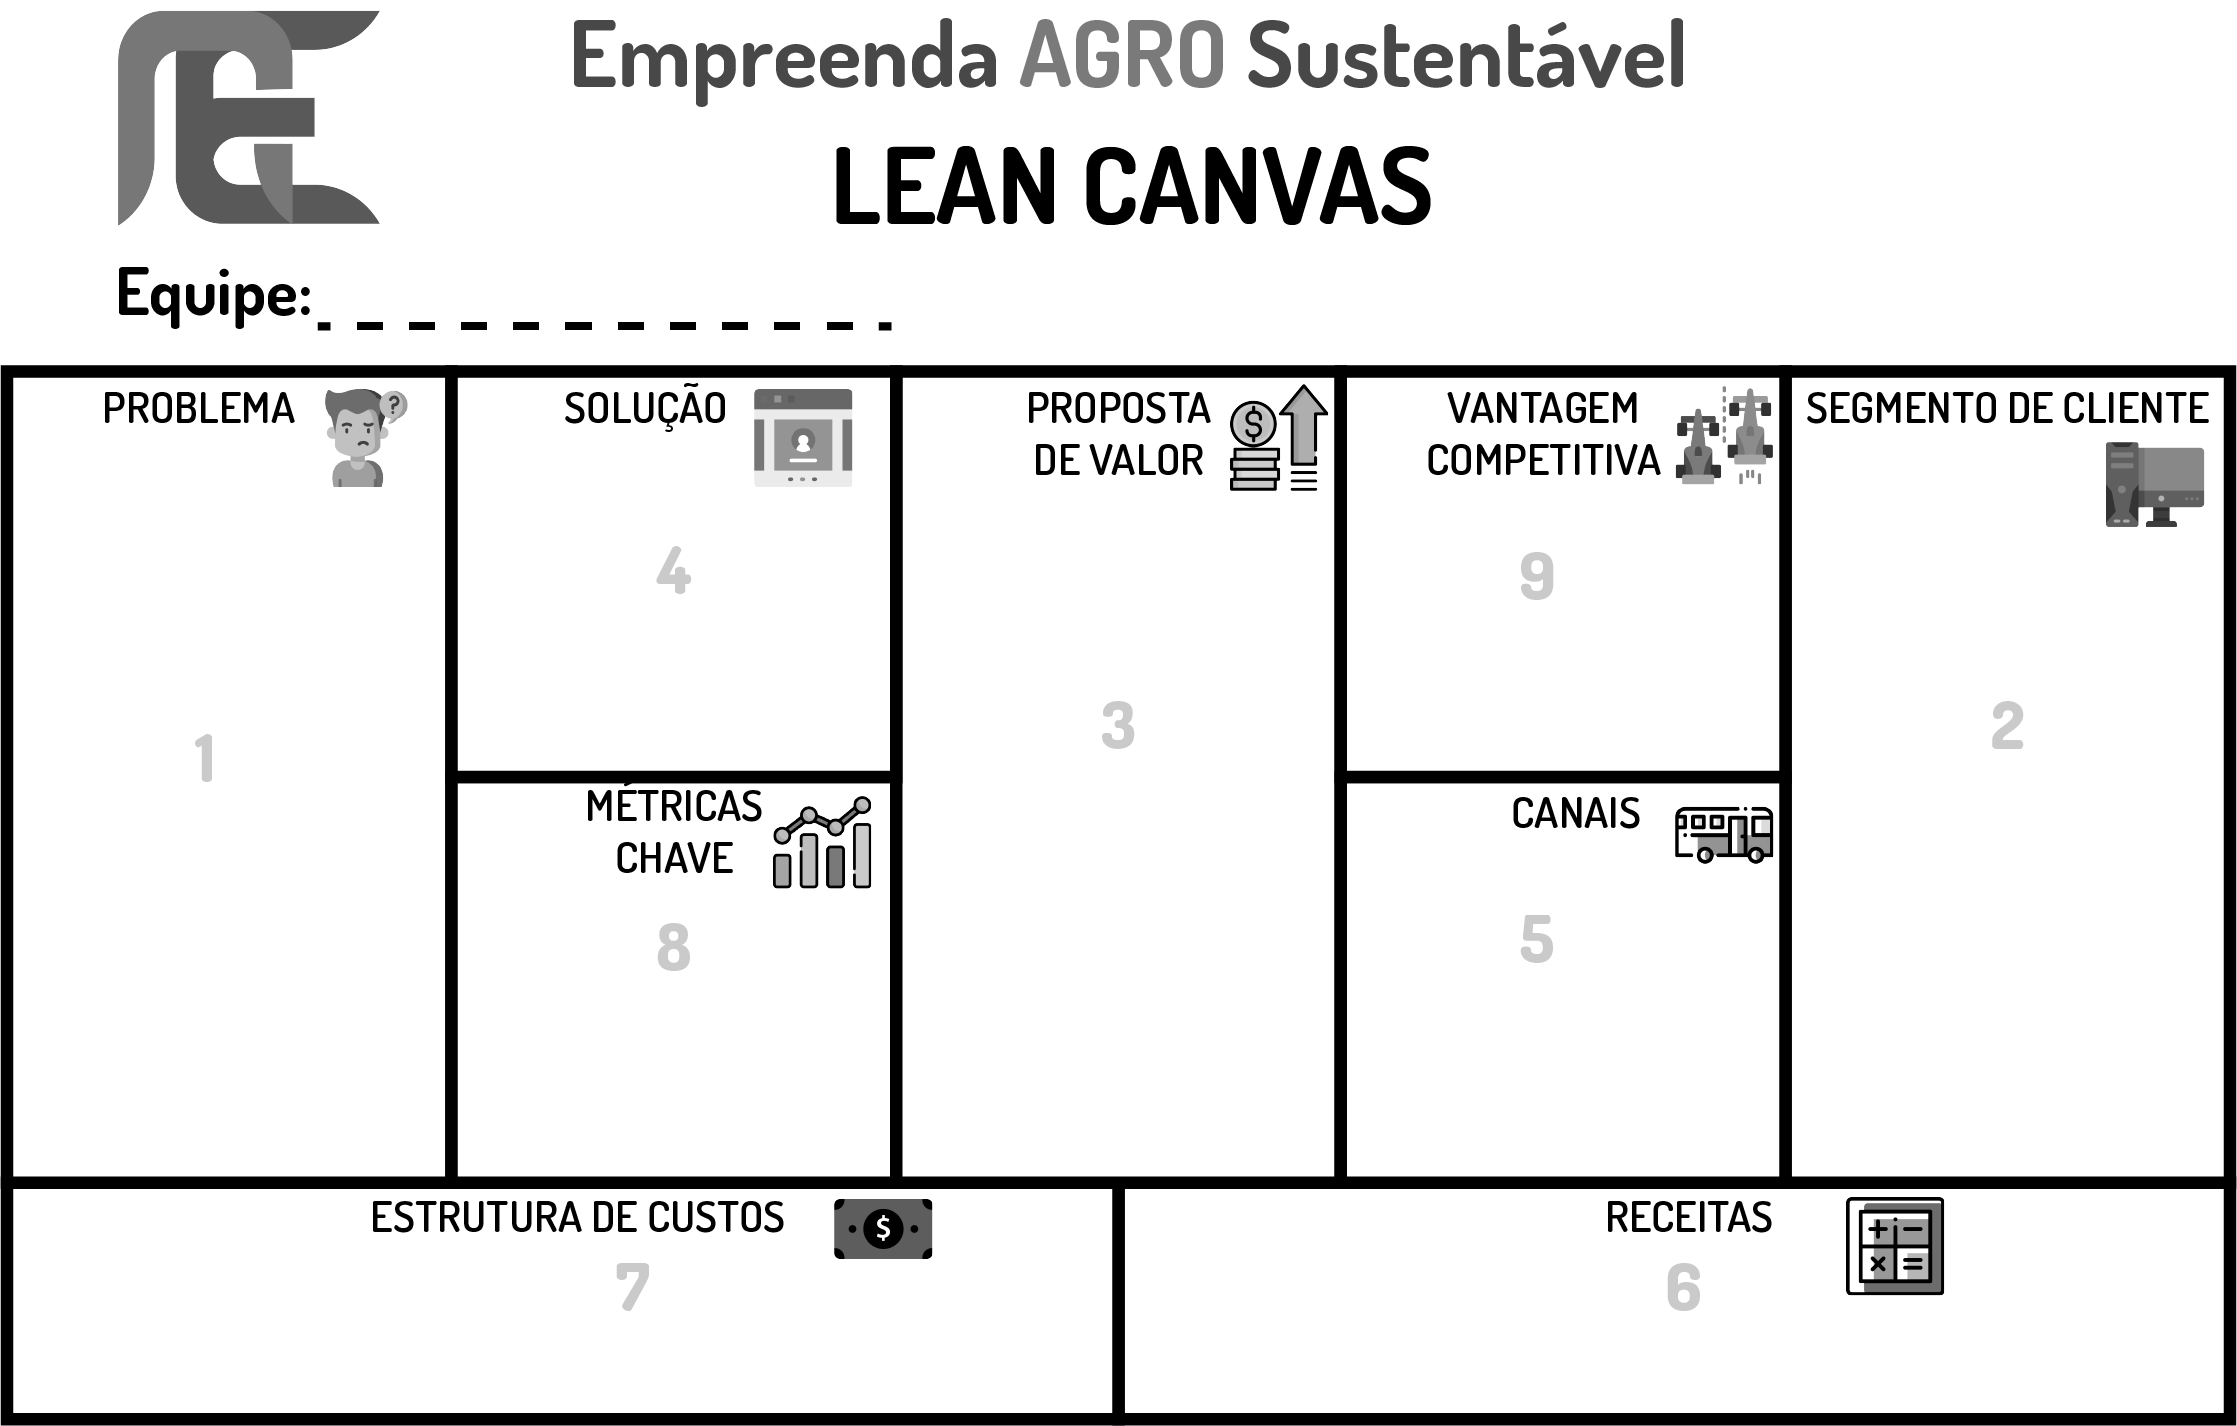
\includegraphics[scale=0.2]{Imagens/canvas.png}
\fonte{Adaptado de: \cite{maurya_running_2012}.}
\label{figura_7}
\end{figure}
\newpage

\subsection{3º Workshop}
 
Neste Workshop será desenvolvido o Makeathon, momento no qual o aluno desenvolverá, de forma prática o seu Mínimo Produto Comercialmente Viável (MVBP sigla em inglês), que segundo \citeonline{aulet_empreendedorismo_2019} é um produto completo o bastante para que um cliente possa ganhar valor com ele, o qual deva possibilitar a demonstração concreta do que se pretende oferecer Figura \ref{figura_32}. 


\begin{figure}[h!]
\centering
\caption{\textbf{Makeathon Empreenda Agro Sustentável}}
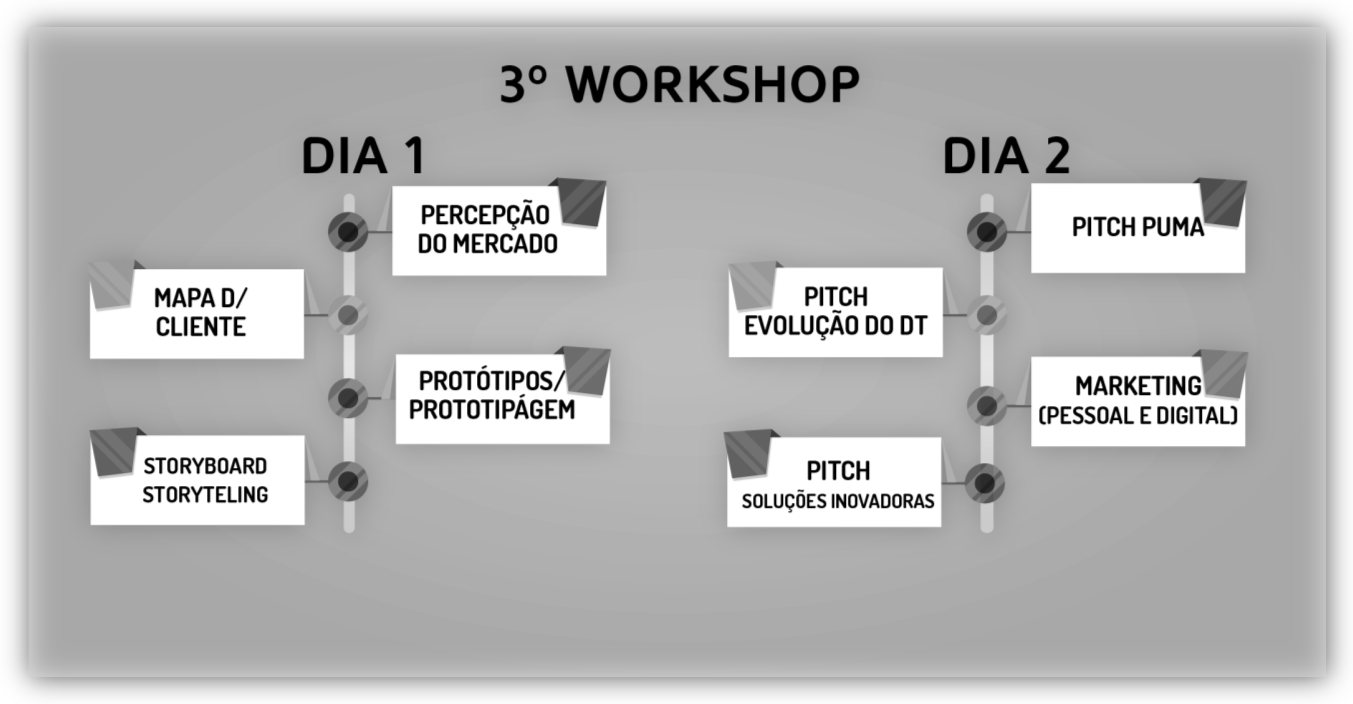
\includegraphics[scale=0.4]{Imagens/workshop-03.png}
\fonte{Adaptado de: \cite{maurya_running_2012}.}
\label{figura_32}
\end{figure}



\subsection{4º Demoday}

E por fim o projeto terá como conclusão o dia de demonstração comercial chamado aqui de Demoday (Figura \ref{figura_33}), será o dia dedicado a demonstrar o quão inovador e interessante é o empreendimento em que foi desenvolvido pelas equipes durante todo o programa.


\begin{figure}[h!]
\centering
\caption{\textbf{Demoday Empreenda Agro Sustentável}}
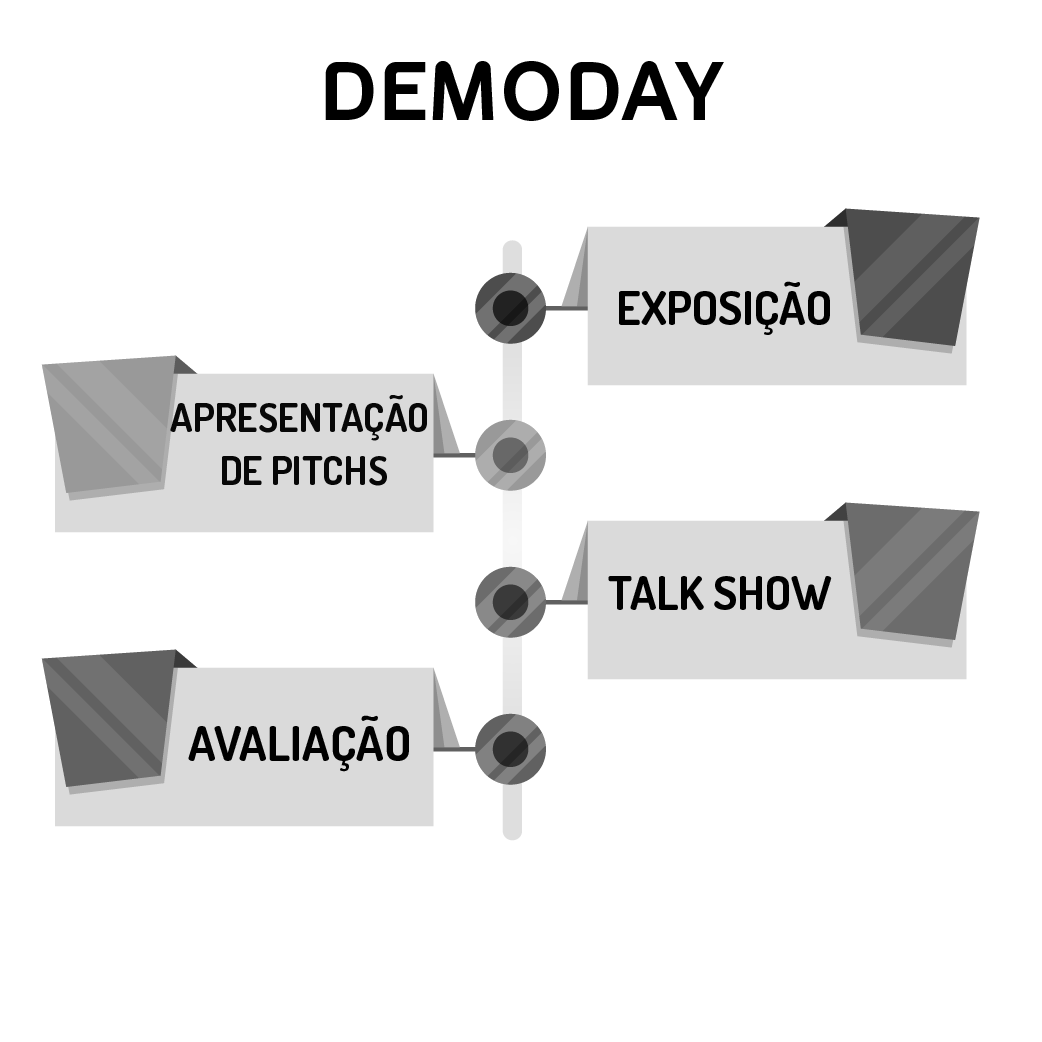
\includegraphics[scale=0.4]{Imagens/workshop-04.png}
\fonte{Adaptado de: \cite{maurya_running_2012}.}
\label{figura_33}
\end{figure}



\section{Mobilização das equipes}

Inicialmente serão abertas vagas para estudantes do curso de graduação, ligadas aos cursos de Ciências Agrárias da Universidade Federal de Sergipe-UFS, onde as inscrições serão realizadas por equipe, desde que preencham os seguintes critérios:

	
\begin{itemize}
\item{Estarem regularmente matriculados e cursando quaisquer dos cursos e ao menos um aluno ligado as ciências agrárias;}
\item{Comprovarem disponibilidade de tempo para participação em todas as oficinas programadas;}
\item{Lidar com trabalhos em equipe.}
\end{itemize}

Objetiva-se o alcance de \textbf{120 alunos} participantes efetivos no programa, o qual será considerado o número de amostra para a pesquisa. Para delimitação das equipes foram elencadas 12 cadeias produtivas  prioritárias e áreas de desenvolvimento agrário destacado-se:

\begin{multicols}{2}
\centering
    \begin{itemize}
    \item{Agricultura Sustentável;}
    \item{Alimentos;}
    \item{Aplicações Molibe}
    \item{Automatização Agrícola}
    \item{Biotenologia}
    \item{Economia Criativa}
    \item{Fitoterapia}
    \item{Higiene/Produtos de beleza}
    \item{Turismo}
    \item{Pecuária Verde}
    \item{Tecnologias gerais}
\end{itemize}
\end{multicols}

\section{Questionário para análise de Campo}

A utilização de um método de pesquisa em uma dissertação depende da escolha de um modelo mais adequado ao problema da pesquisa e os objetivos pretendidos.

Assim, esta pesquisa será desenvolvida com caráter descritivo tendo como base o método de pesquisa \textit{Survey} descritivo, uma vez que este método busca contribui para o conhecimento geral de uma área particular de interesse, pois, envolve uma coleção de informações de indivíduos por meio de questionários e entrevistas sobre suas atividades ou sobre si mesmos \cite{forza_survey_2002}, como também diversos experimentos sobre o empreendedorismo na América Latina têm utilizado \textit{Surveys} realizados em residências ou com apelo direto aos donos de empresas para a coleta de dados, assim como em meios acadêmicos \cite{lima_ser_2015}. Na Figura \ref{figura_8} é possível compreender as fases da tendo como critério a pesquisa do tipo \textit{Survey}.

\begin{figure}[!htb]
\centering
\caption{\textbf{Fases da pesquisa tipo \textit{Survey}}}
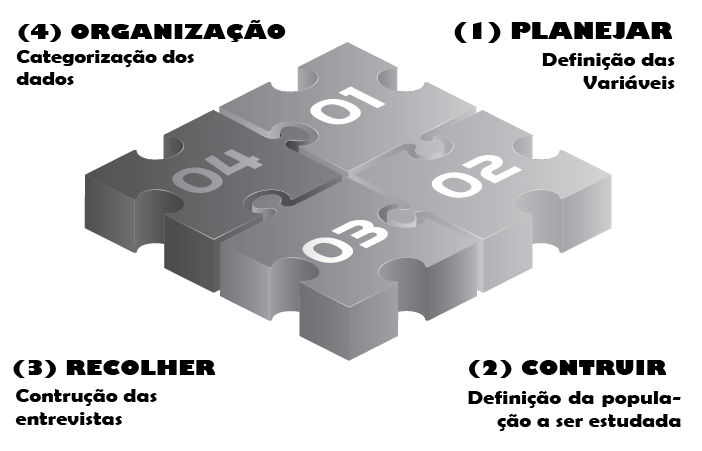
\includegraphics[scale=0.4]{Imagens/survey.png}
\label{figura_8}
\fonte{Adaptado de \cite{moser_survey_2017}.}
\end{figure}

Desta forma, a pesquisa utilizará de um \textit{Survey} descritivo para analisar o potencial do comportamento empreendedor e a competências Empreendedoras, dos acadêmicos dos cursos de graduação em Ciências Agrárias inscritos no Programa Empreenda AGRO Sustentável, utilizando como fator indutor para melhoria o programa de extensão Empreenda Agro Sustentável a partir do modelo \textit{Global University Entrepreneurial Spirit Students’ Survey} (GUESSS), conhecido nacionalmente por Estudo GUESSS. Esta ferramenta de ensaio acadêmico que busca caracterizar o espírito, as atividades e as intenções empreendedores de estudantes universitários, de todos os níveis de aprendizagem e em todos os cursos universitários, bem como as condições de ensino e apoio a atividades empreendedoras. A pesquisa GUESS é realizada internacionalmente,  que em 2018 alcançou mais de 208.000 estudantes de mais de 3.000 universidades em 54 países inclusive no Brasil \cite{sieger_global_2018}.  Seu  principal  objetivo  é  acompanhar  indicadores perceptivos   de   variáveis   de   nível individual   e   contextual   do   ambiente   universitário, relacionados ao empreendedorismo entre estudantes de nível superior.

O questionário apresenta 5 conjuntos de questões dos mais diversos contextos relacionados ao empreendedorismo, medindo diferentes elementos do empreendedorismo e comportamento empreendedor no meio educacional tanto vindo dos discentes quanto dos docentes. O instrumento de pesquisa que será utilizado neste experimento foi composto por Cinco blocos de questões de múltipla escolha baseadas principalmente em escalas de cinco ou sete possibilidades. 

As perguntas iniciais têm por objetivo de traçar o perfil dos alunos entrevistados, tais como: gênero, faixa etária, curso vinculado e o perfil de interesse nas áreas de ensino ligadas ao empreendedorismo sustentável tal questionário foi baseado nos experimentos desenvolvido por \citeonline{lima_educacao_2014}. 


O Primeiro bloco contendo 11 questões abordará a ligação da família e o apoio familiar no empreendedorismo, tendo como alternativas, partido do “Discordo totalmente” a “Concordo totalmente”.

O Segundo conjunto e composto por 7 questões que analisam a intenção empreendedora do aluno da quais segue uma proporção partindo da resposta, tendo como alternativas, partido do “Discordo totalmente” a “Concordo totalmente”.

O Terceiro conjunto trata sobre os interesses dos alunos por disciplinas e atividades relacionadas ao empreendedorismo.

O Último conjunto é composto por 10 questões relacionadas a autoeficácia e a intenção em ter sua própria empresa ou ser autônomo composta por questões de múltipla escolha partindo da alternativa “Completamente Inseguro” a Completamente Seguro”. A figura \ref{figura_9} apresenta o universo das dimensões que serão conduzidas nesta pesquisa.


\begin{figure}[!htb]
\centering
\caption{\textbf{Modelo sobre universo das dimensões estudadas nesta pesquisa sobre a intenção empreendedora}}
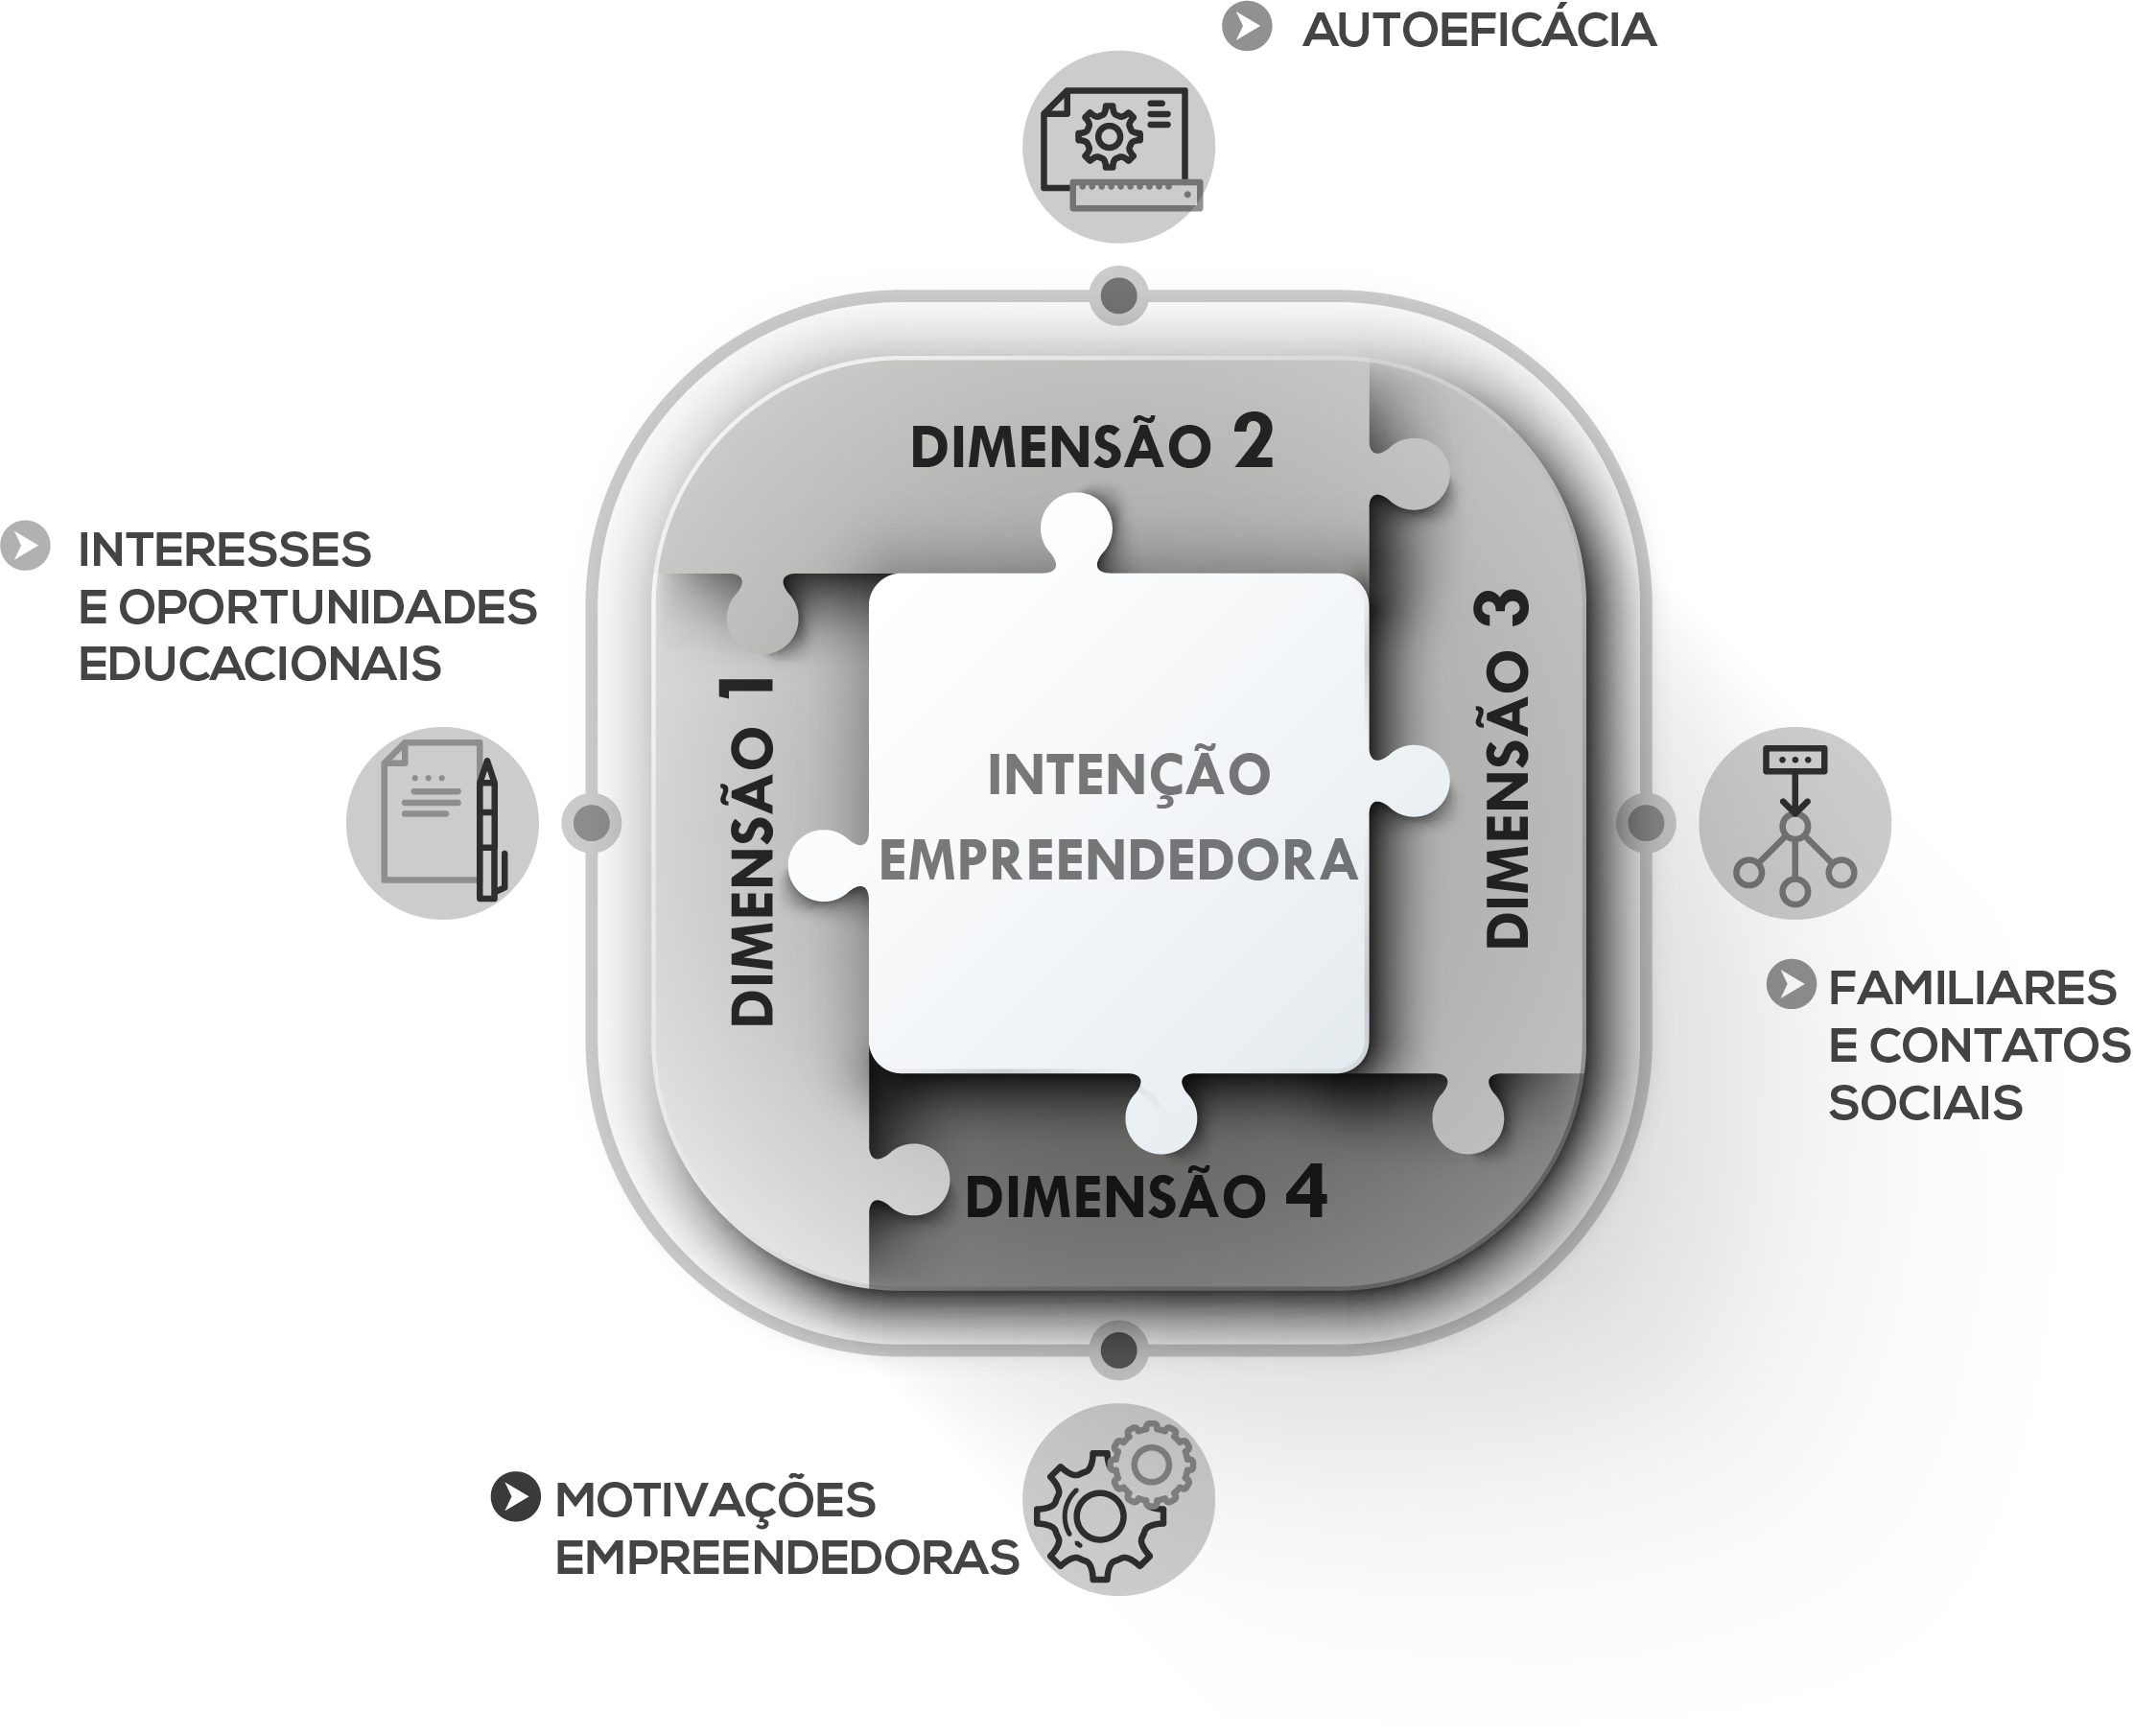
\includegraphics[scale=0.3]{Imagens/intencao_empreendedora.png}
\fonte{Adaptado de \cite{vale_motivacoes_2014}.}
\label{figura_9}
\end{figure}
\newpage

Desta forma a pesquisa caracteriza-se como uma pesquisa de levantamento \textit{Survey} do tipo Descritivo sob corte Longitudinal, já que \citeonline{tormen_potencial_2005} descreve que este tipo de instrução se destaca por compreender uma amostra expressiva em relação ao universo pesquisado. 

\section{Universo da Pesquisa}

O universo desta pesquisa é composto por \textbf{1.143 discentes} ativos dos cursos de graduação nas áreas de agrárias da Universidade Federal de Sergipe (UFS): Engenharia Agronômica, Engenharia Agrícola, Zootecnia, Engenharia Florestal, Medicina Veterinária e Engenharia de Pesca, dados contidos no relatório estatístico de matrículas 2019 da instituição, \cite{campelo_ufs_2018}. É importante considerar que esta pesquisa não considerou classe social local de ensino anterior, e desempenho acadêmico do aluno durante a graduação.

\section{Análises Estatísticas}


Buscando quantificar a homogeneidade das questões, foi utilizado uma análise fatorial e análise de variância multivariada buscando aglutinar as variáveis de cada questão em fatores. Tais fatores forão preparados com o uso da a análise de fatores ortogonais, com rotação Varimax, por meio do método de esfericidade Bartlett e KMO com o nível de significância p < 0,05, este ensaio tem o objetivo de aglutinar em fatores únicos os dados obtidos com diferentes itens de escala do questionário \cite{hair_multivariate_2006}. Esta pesquisa levará em consideração quatro conjuntos de variáveis aglutinados que influenciam na natureza da resposta empreendedora, lembrando que diversos autores abordam diferentes pontos sobre esta temática, visto que este programa se comporta como uma fase de pre aceleração, abordaremos os fatores que podem ter comportamento de conjunto de variáveis independentes, quando submetidas à participação dos alunos no programa, a Figura \ref{figura_9} representa as 4 dimensões estudadas:


\begin{itemize}
\item {Interesse em conteúdos relacionados a educação empreendedora;}
\item {Dimensão da Autoeficácia dos estudantes;}
\item {Dimensão da intenção pretensão ao empreendedorismo dos estudantes;}
\item {Dimensão da participação familiar e influência de terceiros no desenvolvimento empreendedorismo;}
\end{itemize}

Buscando analisar a dimensão \textbf{Interesse em conteúdos relacionados a educação empreendedora;} após a participação no programa, será utilizado uma Análise de Variância Multivariada (MANOVA) caso os dados satisfaçam as exigências para tal teste. A MANOVA é uma técnica estatística que analisa independentemente grupos distintos de amostras buscando avaliar as diferenças entre as médias por grupos. A MANOVA tem por objetivo verificar diferenças de grupos de variáveis categóricas (independentes) quanto aos seus impactos sobre diversas variáveis métricas (dependentes) em paralelo  \cite{hair_alise_2009}. 

Este modelo aplica-se a esta pesquisa, pois ela tem por objetivo avaliar as alterações quanto ao perfil empreendedor em grupos de alunos participantes do Programa de extensão Empreenda Agro Sustentável. Desse modo, é possível avaliar se as diferenças entre os níveis médios dos grupos captados pela \textit{}{survey} são significativas entre os grupos e dentro dos grupos \cite{rocha_avaliacao_2014}. 

A hipótese nula aqui apresentada será utilizada para condução deste experimento. Com a rejeição desta, a hipótese alternativa é comprovada \ \cite{hair_alise_2009}.

\textbf{H0:} Não há diferença entre as médias das medidas que averíguam o perfil empreendedor entre os alunos participantes do Programa de extensão Empreenda Agro Sustentável.

\textbf{H0} Não há diferença entre as médias das medidas que averíguam o perfil empreendedor entre os alunos participantes do Programa de extensão Empreenda Agro Sustentável.



Para o processamento dos dados será utilizado o Software IBM SPSS \cite{ibm_corp_ibm_2017}. 


\section{Tamanho da amostra}

Muitas  vezes  não  se  faz necessário,  ou  é não é possível,  dispor  de toda a população objetivo  do  projeto. Desta forma se faz necessário dispor de uma parte do universo da pesquisa para que seja possível realizar inferências confiáveis da população total \cite{marino_manual_2003}.

Para que seja possível a análise populacional de forma fidedigna, e selecionada uma amostra de tal população. Amostra é o número de pessoas a que serão entrevistadas nesta pesquisa. Esse número tido inicialmente como o número máximo de capacidade de condução efetiva do programa, partindo do universo pesquisado (CCAA) ele representa 10,5\% dos alunos ativos no centro, número satisfatório para avaliação de projetos sociais segundo \citeonline{marino_manual_2003}, segundo o autor quando o número total do grupo próximo a 1.000 é sugerido uma amostra de 50 a 100 participantes. 

A amostra desta pesquisa compreenderá \textbf{120 discentes} que participarem do Programa Empreenda Agro Sustentável que responderão o questionário instrumento de pesquisa que serão aplicados durante os Workshops. Tais Workshops ocorrerão nos meses de agosto, outubro e dezembro de 2019. Tal instrumento será aplicado presencialmente. 


\section{Considerações Éticas}

Por critérios éticos precedendo ao início do questionário, foi inserido um Termo de Consentimento Livre e Esclarecido (\textbf{TCLE}), composto por esclarecimentos sobre a pesquisa, além da solicitação de autorização para o uso dos dados e por ventura imagem que seja necessária ao desenvolvimento do experimento. questionário aplicado nesta pesquisa atende os termos das Resoluções n. 466 de 12 de dezembro de 2012 do Conselho Nacional de Saúde \cite{cns_resolucao_2012}, o qual por se tratar de pesquisa com seres humanos foi submetido ao Comitê de Ética em Pesquisa Envolvendo Seres Humanos (\textbf{CEP}) e a Comissão Nacional de Ética em Pesquisa (\textbf{Conep}) por meio da plataforma Brasil Saúde sendo \textbf{APROVADO} sob o número do Certificado de Apresentação para Apreciação Ética \textbf{CAAE: 23853219.4.0000.5546}.





\chapter{RESULTADOS E DISCUSSÃO}

Entender como a contribuição acadêmica influencia na intenção inicial da carreira empreendedora é de grande interesse para centros acadêmicos, profissionais e educadores em empreendedorismo. Desta forma os resultados desta pesquisa encontram-se divididos em seções, que atendem aos objetivos propostos no estudo.
Inicialmente são apresentadas descrições que caracterizam os dois perfis estudados
(pré-programa e pós-programa) em relação às variáveis e as comparações entre os grupos. Posteriormente serão apresentadas as inovações produzidas pelos alunos participantes durante o decorrer do programa.



\section{Materiais de apoio para desenvolvimento do aprendizado teórico dos conteúdos: Aplicativo Empreenda Agro Sustentável}

Muitos aplicativos móveis agrícolas pagos e gratuitos foram desenvolvidos para o meio rural, abrangendo diversas áreas dentro e fora da propriedade rural (SILVA et al., 2017). A tecnologia da informação apresenta grandes potencialidades para auxiliar produtores rurais e profissionais da área na tomada de decisões estratégicas. Todavia, para o profissional das ciências agrárias tomar decisões assertivas, não basta apenas manusear a Tecnologia da Informação aplicada ao agronegócio, é   necessário   mudar   a   concepção   dos   processos   a   partir   de   sua informatização (FERRAZ; PINTO, 2017).
Desta maneira, o aplicativo foi desenvolvido para ser ferramenta portátil, acessível e utilizável por acadêmicos da ciências agrárias no sentido de dar direcionamento educacional em empreendedorismo. 


\subsection{Recursos e funcionalidades do aplicativo}

O aplicativo consiste em uma interface com bancos de dados que permite ao usuário averiguar, de modo interativo, os conteúdos melhor recomendados para o aprendizado da cultura empreendedora para as áreas das ciências agrárias. 
Para o acesso de dados através do dispositivo portátil o mesmo pode ser instalado em alguns cliques, onde o usuário não precisa estar inscrito ou participando do programa, para efetuar o primeiro acesso. É necessário apenas ter disponibilidade de rede de internet local ou móvel, que permita o primeiro download das informações. Após concluir a transmissão de dados para o aplicativo, não se faz necessário ter continuidade da internet para utilizar o aplicativo. 
Durante a execução do aplicativo, tem-se a tela de inicialização que conta com a marca do programa e aplicativo homônimo (Figura \ref{figura_42}a). 
Após, apresenta-se a tela principal (Figura \ref{figura_42}a) do aplicativo que exibe uma lista de botões para selecionar o tipo de conteúdo de interesse do usuário. Estas funcionalidades podem ser acessadas por um menu lateral deslizante (Figura \ref{figura_42}a), facilitando assim o manuseio do aplicativo pelo usuário final. 


\begin{figure}[H]
\FloatBarrier
\center
\caption{\textbf{Aplicativo Empreenda Agro Sustentável}}
\subfigure[ref1][Tela inicial]{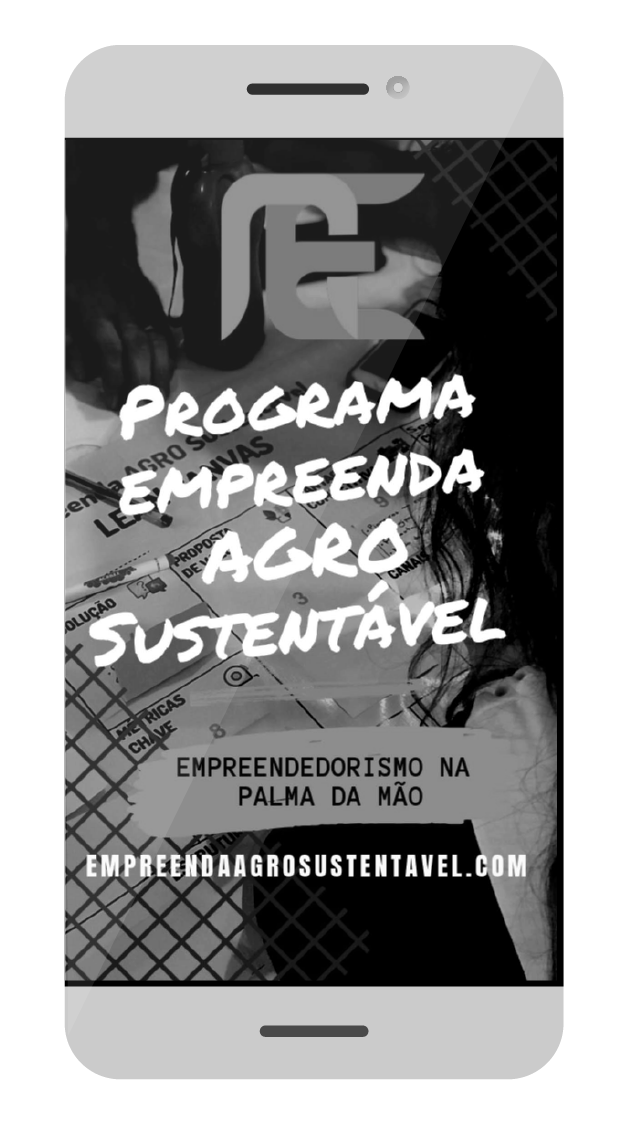
\includegraphics[scale=0.2]{Imagens/aplicativo_login.png}}
\qquad
\subfigure[ref2][Tela Principal]{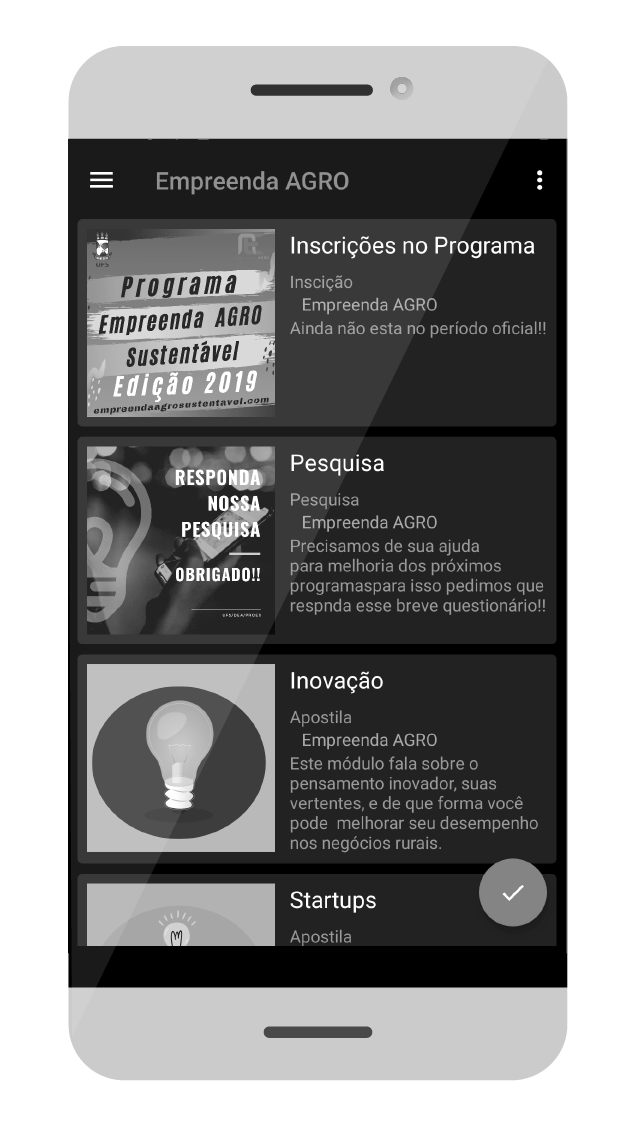
\includegraphics[scale=0.2]{Imagens/aplicativo_1.png}}
\qquad
\subfigure[ref3][\textit{Drawer list}]{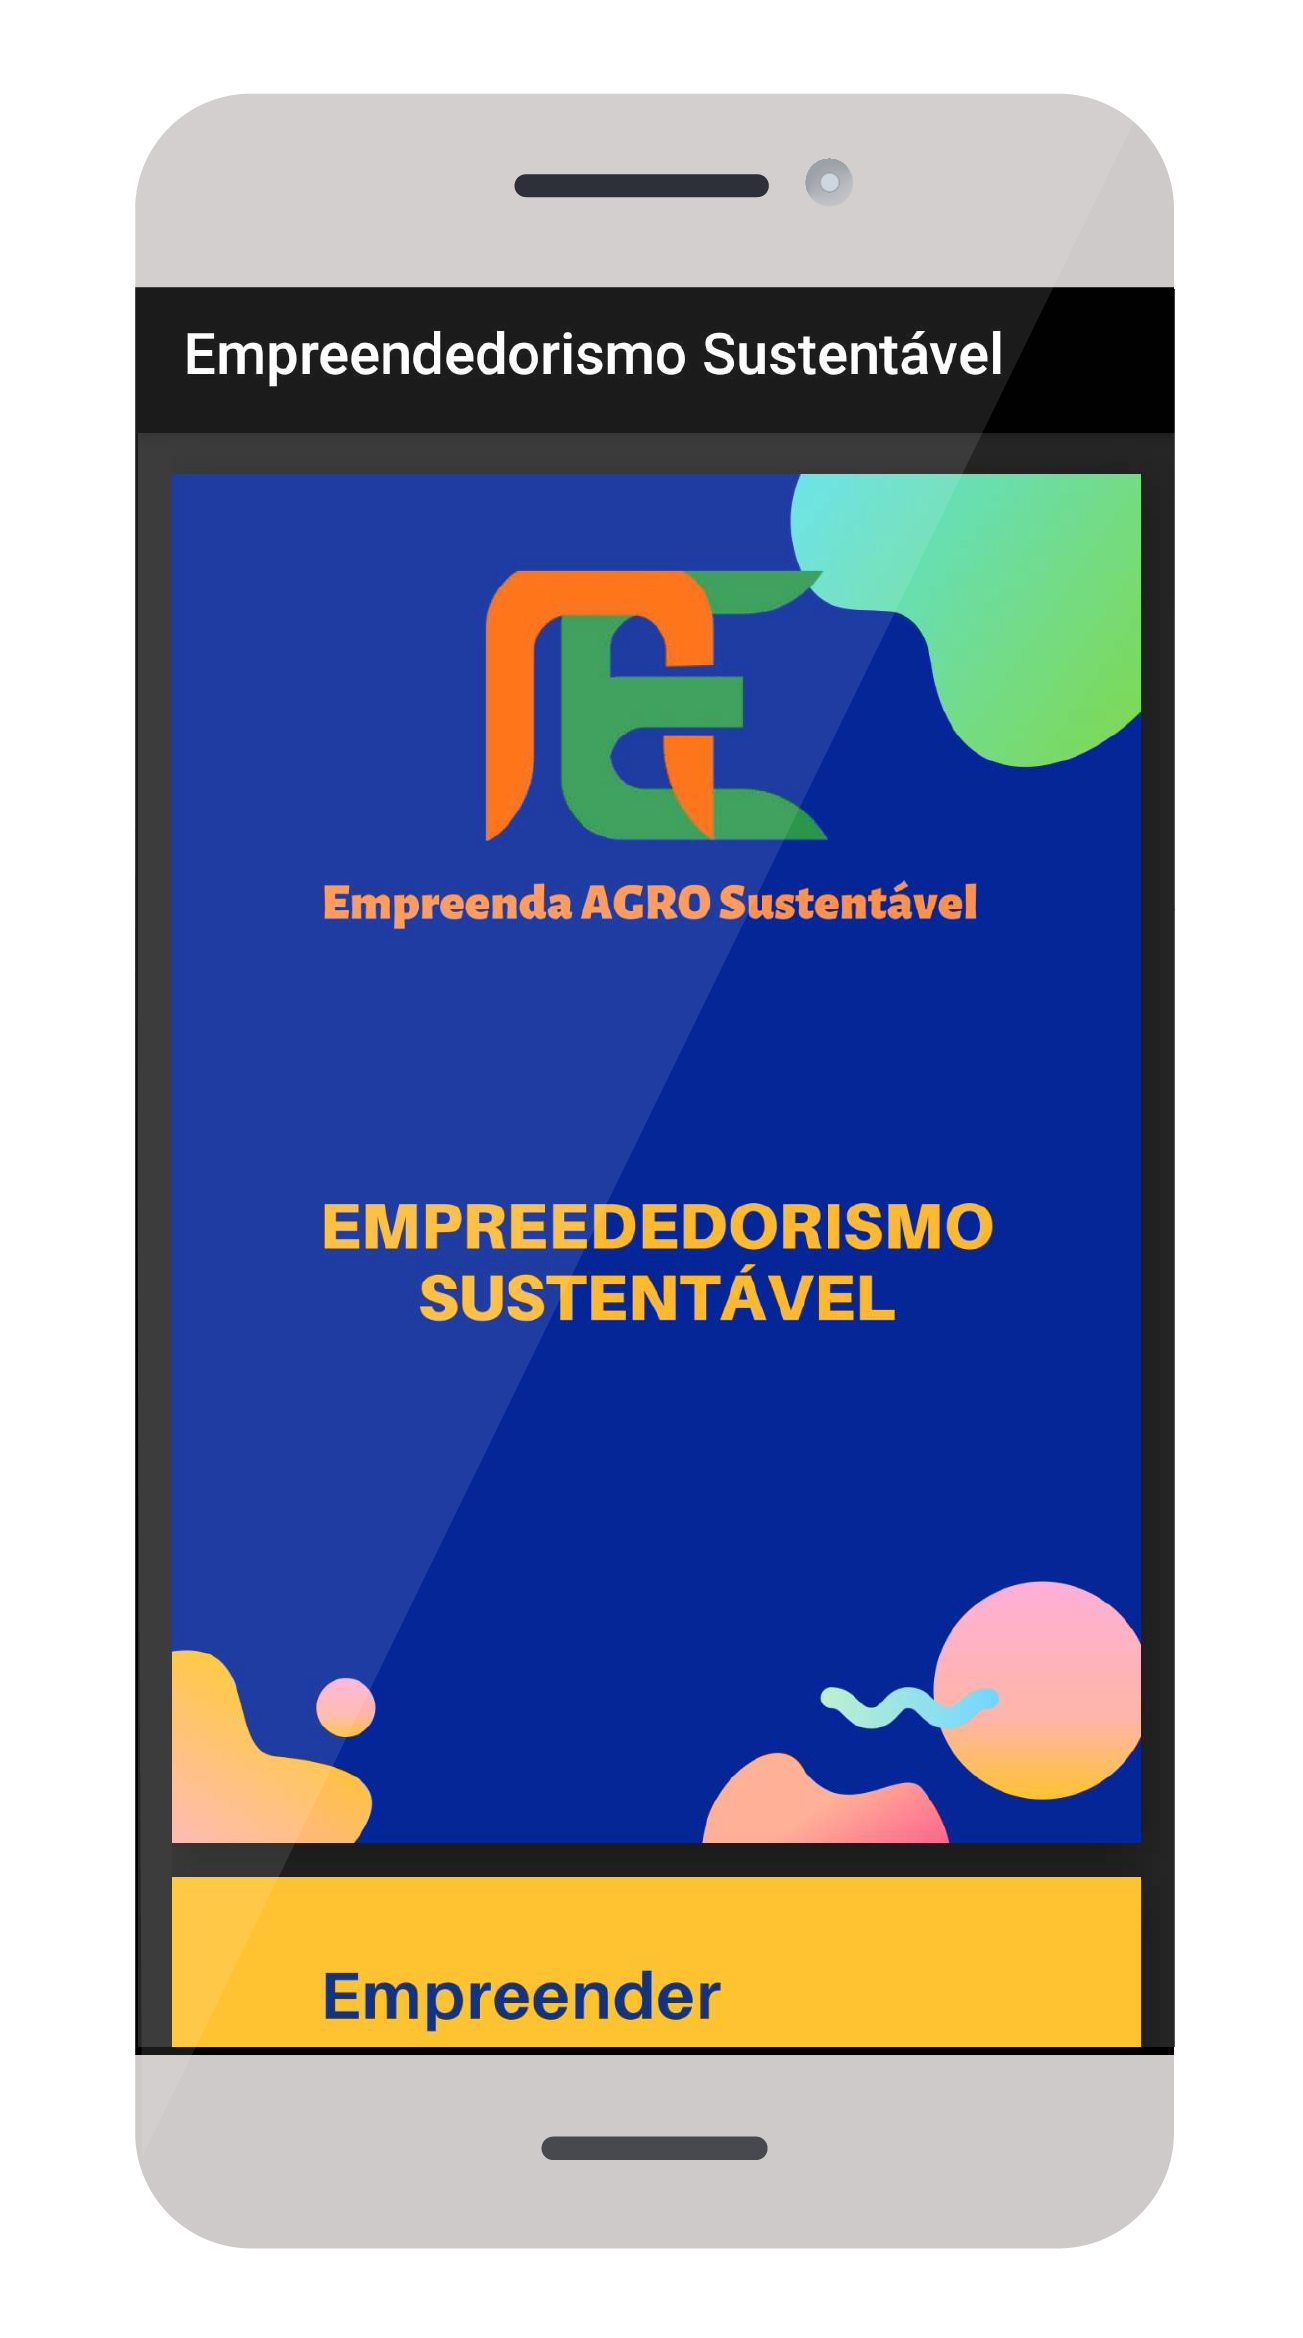
\includegraphics[scale=0.2]{Imagens/aplicativo_3.png}}
\fonte{Próprio Autor}.
\label{figura_42}
\end{figure}



Todas as informações sobre o software assim como o sobre os conteúdos de apoio a serem abordados estão disponíveis, em todos os tipos de mídias (áudio, vídeo e escrito), já que o aplicativo conta com diversos formatos de mídias digitais e links com outros canais de divulgação como exemplo: O streaming Spotify (Figura \ref{figura_44}a), o Youtube.com e o site de notícias sobre empreendedorismo Exame \ref{figura_44}a).  Para os dados escritos, o usuário poderá exportar em formato .pdf dos dados presentes no dispositivo portátil (Figura \ref{figura_44}c).

Estas funcionalidades podem ser acessadas pelo menu lateral deslizante chamado de \textit{Drawer list} (Figura \ref{figura_42}c), facilitando assim o manuseio do aplicativo pelo usuário final. 

\begin{figure}[H]
\FloatBarrier
\center
\caption{\textbf{Aplicativo Empreenda Agro Sustentável}}
\subfigure[ref4][Podcasts]{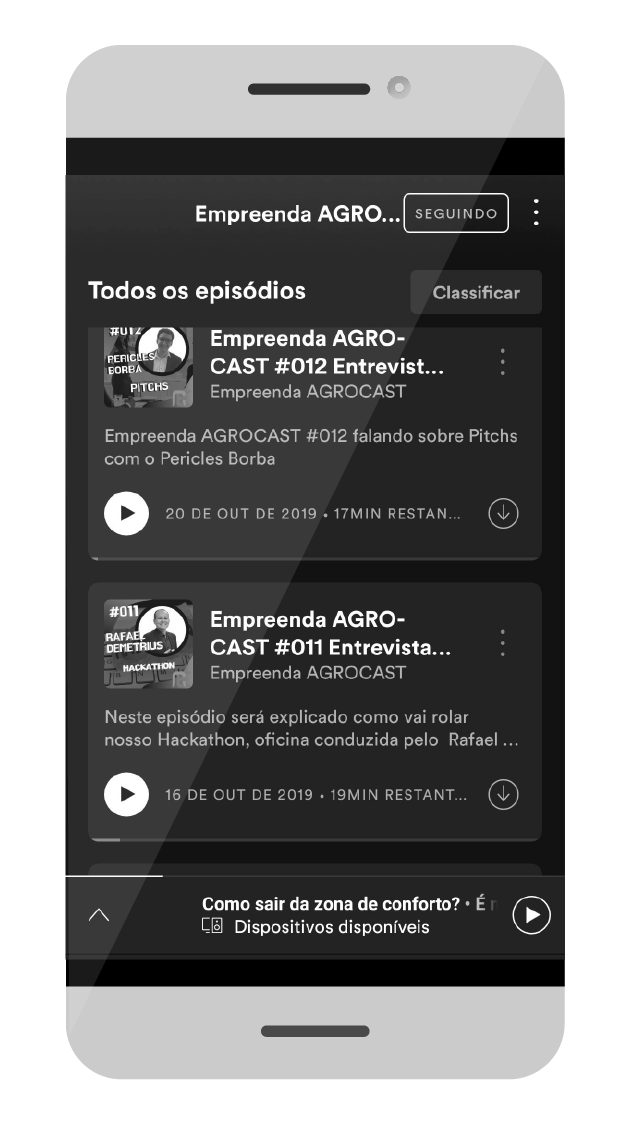
\includegraphics[scale=0.2]{Imagens/aplicativo_4.png}}
\qquad
\subfigure[ref4][Notícias sobre empreendedorismo]{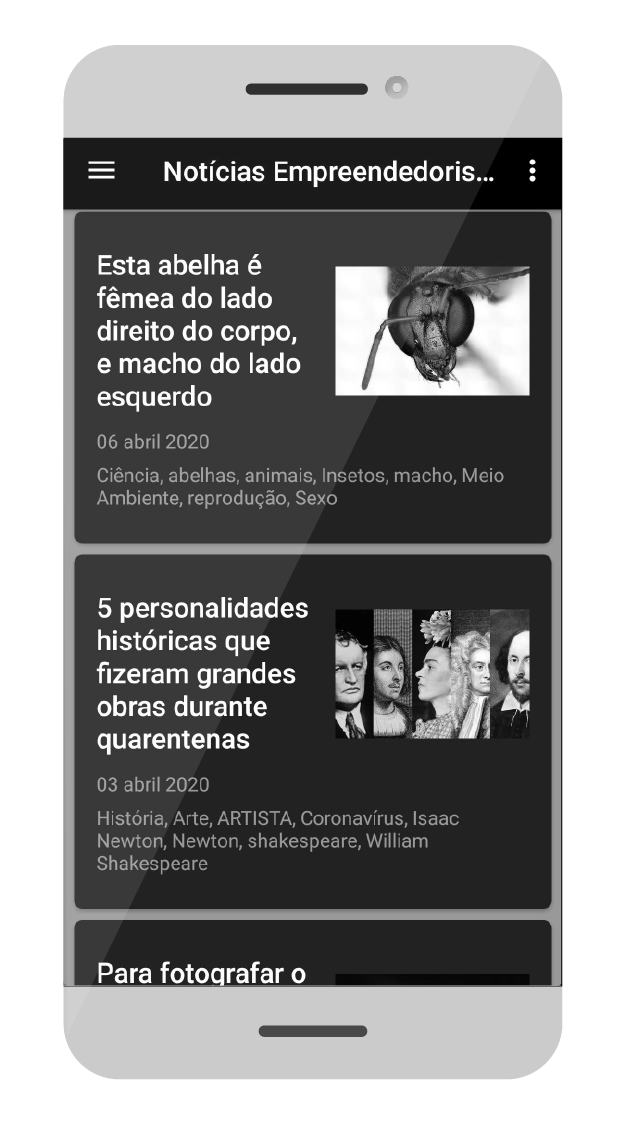
\includegraphics[scale=0.2]{Imagens/aplicativo_5.png}}
\qquad
\subfigure[ref4][Conteúdos escritos]{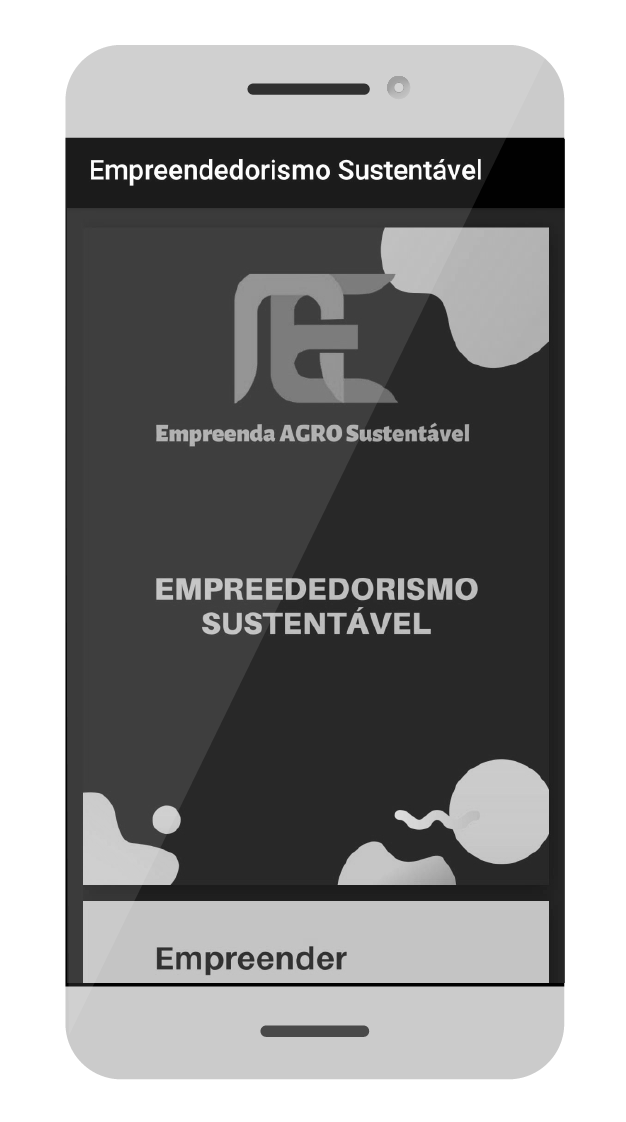
\includegraphics[scale=0.2]{Imagens/aplicativo_6.png}}
\fonte{Próprio Autor}.
\label{figura_44}
\end{figure}


\subsection{Teste de usabilidade do aplicativo}

Os principais critérios de inclusão para os usuários testadores foi o acesso a participação do programa e um telefone Android, pois o aplicativo foi desenvolvido apenas em uma plataforma Android, o download do aplicativo foi disponibilizado de forma grátis por meio da loja de disponibilidade de aplicativos Google Play.
Na Figura 6 é possível ver a serie temporal dos downloads ao aplicativo por meio da plataforma Google Play. A maior quantidade de versões operacionais do sistema Android foi a versão 9.0 tendo alcançando 32 aparelhos ativos desde o início do lançamento (Figura \ref{figura_43}).

\begin{figure}[H]
\caption{\textbf{Série temporal dos dispositivos ativos desde o lançamento no dia 01 de outubro de 2019 até o mês de abril de 2020.}}
\centering
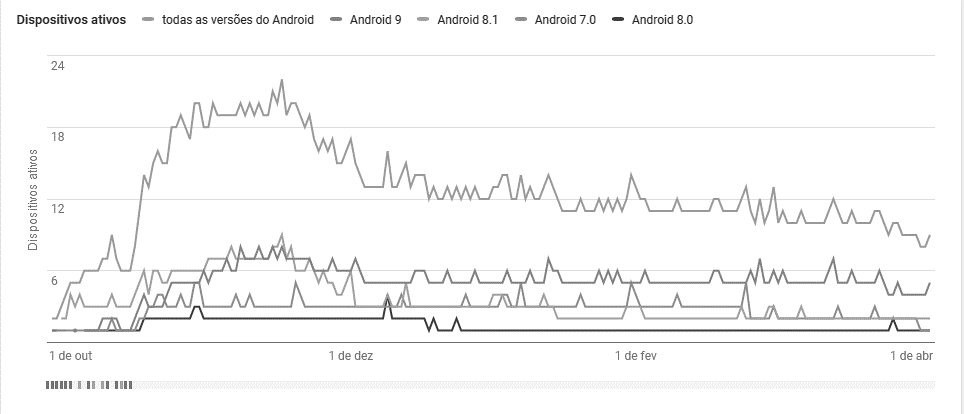
\includegraphics[scale=0.6]{Imagens/dispositivos_instalados.png}
\fonte{ \citeonline{google_developer_google_2020}}
\label{figura_43}
\end{figure}

Para o fluxo de atividade da aplicação, foi deixado aos usuários a manipulação de forma orgânica dos conteúdos, a fim de que fosse possível observar eventuais falhas durante o uso e requisição de conteúdos da plataforma. 
As tarefas específicas dos testadores de aplicativos incluíram o acesso a abas, abertura de links resultantes de dados externos; leitura fluida dos materiais disponíveis em pdf, acesso livre aos conteúdos disponíveis em vídeos, (nenhum limite foi definido para a quantidade de dados a serem registrados no aplicativo) e a navegação geral do aplicativo, de forma fluida e rápida.
 Qualquer falha de acesso aos dados ou tempo de atraso na resposta do aplicativo durante o lançamento e o uso, “troca de tela”, usando o teclado deslizante e os botões da tela de toque dos aplicativos também foram monitorados, seguiram procedimentos de feedback por meio da plataforma Google Play Console, os procedimentos utilizados para teste do aplicativo foram os mesmos descritos por \cite{adu_development_2020}.

O APP Empreenda Agro Sustentável é um aplicativo que foi produzido pelo programa com o propósito de auxiliar os alunos dos cursos de ciências agrárias participantes, ao aprendizado da educação empreendedora por meio de conteúdos dinâmicos e direcionados a área de negócios no meio rural, tais como: Materiais informativos, Vídeo aulas, podcasts.
O aplicativo também é indicado para profissionais que tenham interesse de aprender mais sobre o desenvolvimento de negócios sustentáveis e escaláveis.
A implementação destas funcionalidades dentro do aplicativo seguiu satisfatoriamente as solicitações dos usuários,.
Buscando cumprir os requisitos de aquisição de direito e propriedade autoral o aplicativo foi registrado no Instituto Nacional de Propriedade Industrial INPI sob número de registro \textbf{BR 51 2019 002657 8} e disponível gratuitamente para testes na loja online Google Play Store, de propriedade da Universidade Promotora do Programa.



\section{Alcance da amostra experimental}

No desenvolvimento do programa foram formadas inicialmente 26 equipes que somaram 118 alunos oriundos dos cursos de graduação do Centro de Agrárias e Aplicadas além de outros cursos como: Artes Visuais, Administração, Design Gráfico, Engenharia Química, Engenharia de Produção, Marketing e Ecologia.
Os dados coletados revelam que, nas 115 respostas válidas que compõem a amostra a faixa etária no período de inscrição, apresentavam 75,4\% dos estudantes com idade menor que 20 anos, 16,1\% apresentaram a intervalo de idades entre 21 e 25 anos, e 59\% tinham idade maior que 25 anos (Tabela \ref{tabela_45}).
 
\begin{table}[H]
\centering
\caption{\textbf{Faixa etária dos alunos participantes do programa}}
\label{tabela_45}
\begin{tabular}{clcc} 
\hline\hline
 \textbf{Dados}                       & \textbf{Faixa etária}  & \multicolumn{2}{c}{~\textbf{Inscritos} }                                                        \\ 
\hline
\multirow{3}{*}{}                     &                        & \multicolumn{1}{l}{\textbf{Frequência (\%)} } & \multicolumn{1}{l}{\textbf{Porcentagem (\%)} }  \\
                                      & \textbf{Menor que 20}  & 89                                            & 75,4                                            \\
                                      & \textbf{De 21 a 25}    & 19                                            & 16,1                                            \\
\multicolumn{1}{l}{\textbf{Válidos} } & \textbf{Maior que 25}  & 7                                             & 5,9                                             \\
\multicolumn{1}{l}{}                  & \textbf{Total}         & 115                                           & 97,5                                            \\ 
\hline
\multicolumn{1}{l}{\textbf{Omissos} } & \textbf{Não informou}  & 3                                             & 2,5                                             \\ 
\hline
\multicolumn{2}{c}{\textbf{TOTAL GERAL} }                      & \multicolumn{1}{l}{118}                       &                                                 \\
\hline\hline
\end{tabular}
\fonte{O autor}
\end{table}


O curso com maior participação numérica foi o de Engenharia Agronômica, representando 47,32\% deste total, enquanto os cursos de Engenharia Agrícola, Zootecnia, Engenharia de Pesca e Engenharia Florestal participaram em termos percentuais e respectivamente com 11,61\%, 19,64\%, 4,46\% e 6,25\% do total de estudantes inscritos. Na Figura \ref{figura_10} são apresentados dados sobre a quantidade de alunos inscritos e seus respectivos cursos.



\begin{figure}[H]
\caption{\textbf{Numero de alunos inscritos e percentual por curso no universo total de participantes do Programa.}}
\centering
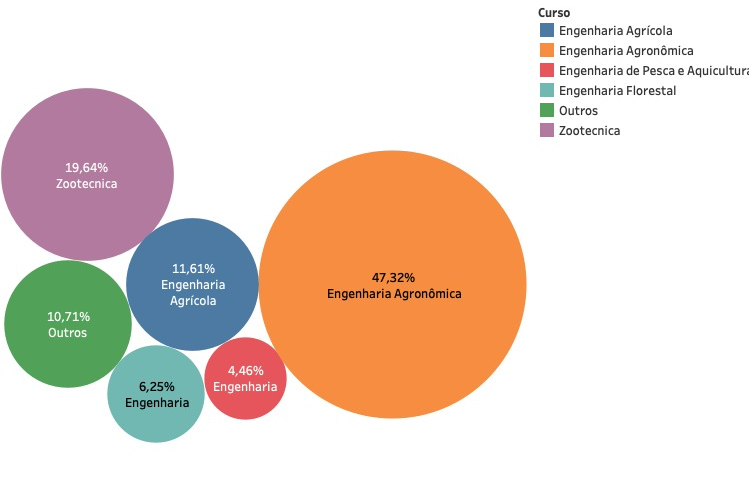
\includegraphics[scale=0.3]{Imagens/inscritos.png}
\fonte{Autoria própria}
\label{figura_10}
\end{figure}



\section{Áreas e cadeias produtivas selecionadas}

A fase de inscrição no do programa alcançou 27 propostas de protótipos e/ou negócios na área rural com foco na agricultura sustentável. Na figura \ref{figura_11} é possível verificar as áreas e cadeias produtivas prioritárias escolhidas. Das quais deram continuidades durante todo o projeto 15 equipes.

\begin{figure}[!htb]
\centering
\caption{\textbf{Áreas e potenciais propostas de negócios escritos}}
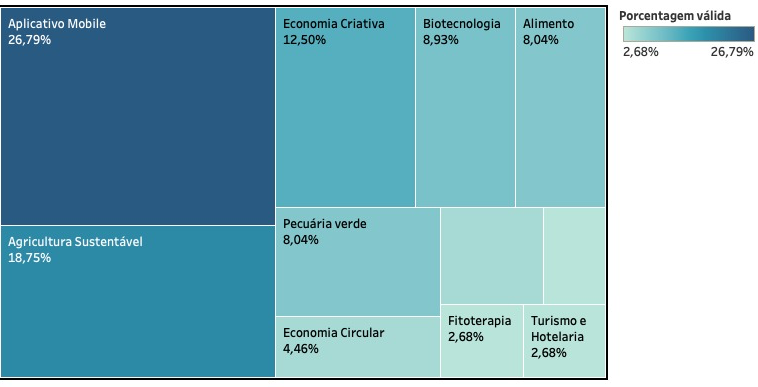
\includegraphics[scale=0.6]{Imagens/propostas_negocios.png}
\fonte{O autor}
\label{figura_11}
\end{figure}



\section{Contextualizando o cenário da prática}


Para a uniformização da linguagem e terminologias tratadas nesse artigo, de agora em diante, não mais faremos referência ás “oficinas”, que substituímos por “Workshops”, uma vez que foi essa a terminologia utilizada nos textos do projeto submetido á PROEX/UFS, assim como em todo material de divulgação. 

Os encontros com os alunos aconteceram mensalmente, de maneira presencial durante dois dias em dois turnos. A proposta da metodologia contemplou a divulgação semanal de atividades desenvolvidas pelos grupos, a fim de manter o engajamento dos participantes e desenvolvimento das propostas de negócios pensadas ao entrarem no programa. Inicialmente, foi desenvolvido um site \href{http://www.empreendaagrosustentavel.com}{empreendaagroustentavel.com}  para divulgação do programa proposto. A cada Workshop, foram desenvolvidas atividades práticas, obedecendo aos seguintes critérios: Desenvolvimento gradual da ideia de negócio de forma planejada; Desenvolvimento de planos de negócios e planos gerenciais; Desenvolvimento do mínimo produto economicamente viável; Aprendizado e estratégia de apresentação do produto proposto.
 

O indivíduo é o conjunto de seus Conhecimentos, Habilidades e Atitudes (CHA) \cite{dutra_competencias_2004}, conjunto este de grande relevância para um empreendedor, especialmente porque as competências se mostram como parte fundamental da formação do empreendedor nos dias atuais, o qual assume a responsabilidade de agregar valor às organizações \cite{ferreira_conhecimento_2019}, desta forma, se mostra importante o aprendizado contínuo e multidisciplinar para fixação e melhor desenvolvimento dos conteúdos aprendidos. \citeonline{limberger_metodologias_2013} ressalta que, as metodologias ativas proporcionam uma visão reflexiva maior que a apresentada nos métodos tradicionais de ensino: 

\begin{citacao}
[...] Quando o aprendizado ocorre por meio de metodologias ativas, o conhecimento dos estudantes é comparável ao do método tradicional, porém, seu desempenho em relação às suas habilidades e atitudes é superior, reflexo da visão crítico reflexiva proporcionada pelo método.[...] \cite{limberger_metodologias_2013}.
\end{citacao}


Foram promovidos quatro Workshops, nos quais foram abordados, os conceitos de empreendedorismo, ideação, modelo de negócios, marketing, entre outros. As oficinas foram conduzidas através de palestras, a    tividades práticas e dinâmicas, ou seja, metodologias ativas. Os Workshops foram conduzidos no formato de “Jornada” (Figura \ref{figura_17}), ou seja, aos participantes foram apresentados gradativamente a conteúdos e metodologias. 


\begin{figure}[H]
\centering
\caption{\textbf{Jornada Empreenda Agro Sustentável}}
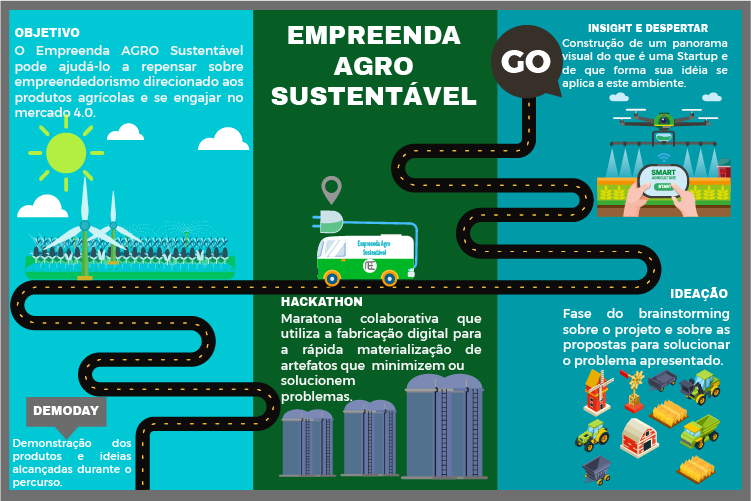
\includegraphics[scale=0.6]{Imagens/jornada.png}
\fonte{O autor}
\label{figura_17}
\end{figure}

Numa sequência encadeada de conteúdos e práticas as equipes formadas, e sempre numa dinâmica proativa, iniciaram a jornada com o “despertar”, que já acontecia antes mesmo da realização do primeiro Workshop, por meio das várias intervenções ainda usando formas remotas de comunicação, que repassaram conteúdo a partir de materiais escritos e podcasts disponibilizados no site do Programa, por meio do link  \href{https://open.spotify.com/show/3c25hRSxvaCFPw6Y3lX3i1?si=9H_fGz_uRgGiFNhAcdr4rQ}{Empreenda AGROCAST}. Orientados pela jornada posta, as equipes foram reunidas para o Workshop inicial em que a etapa do “despertar” ganhava voz, já oportunizando os momentos inicias da “ideação”. Na sequência de Workshops em que o processo de ideação foi evoluindo, com tempo para possível pivotagem, foi então alcançada a etapa de “prototipagem” da jornada. Como etapa final foi então realizado o “Demoday”, em que as equipes apresentaram os seus pitchs, para investidores, concluindo uma jornada com duração de 6 meses.


Numa sequência encadeada de conteúdos e práticas as equipes formadas, e sempre numa dinâmica proativa, iniciaram a jornada com o “despertar”, que já acontecia antes mesmo da realização do primeiro Workshop, por meio das várias intervenções ainda usando formas remotas de comunicação, que repassaram conteúdo a partir de materiais escritos e  podcasts disponibilizados no site do programa \href{https://open.spotify.com/show/3c25hRSxvaCFPw6Y3lX3i1?si=9H_fGz_uRgGiFNhAcdr4rQ}{Empreenda AGROCAST}. Orientados pela jornada posta, as equipes foram reunidas para o Workshop inicial em que a etapa do “despertar” ganhava voz, já oportunizando os momentos inicias da “ideação”. Na sequência de Workshops em que o processo de ideação foi evoluindo, com tempo para possível pivotagem, foi então alcançada a etapa   de “prototipagem” da jornada. Como etapa final foi então realizado o “Demoday”, em que as equipes apresentaram os seus pitchs, para investidores, concluindo uma jornada com duração de 6 meses.


\subsection{Primeiro Workshop}

As atividades foram iniciadas com a abertura do programa feita pela equipe organizadora, na qual foi apresentada a programação dos Workshops, denominada de “A Jornada”. O momento do programa (1º Workshop) teve como foco o desenvolvimento de palestras e oficinas que abordaram temas relacionados ao empreendedorismo, tais como: Startups, Empreendedorismo, comportamento empreendedor e cultura empreendedora, Problemas (segmentação do mercado) segundo as ODS (Objetivos do Desenvolvimento Sustentável) e Agritechs na palestra “Tecnologias digitais e as oportunidades para o Agronegócio”. Como prática tendo como base pedagógica as metodologias ativas, teve o início do desenvolvimento do Lean Canvas, com foco no bloco referente a proposta de valor (Apêndice \ref{app:workshop_1}).



\subsection{Segundo Workshop}


O segundo Workshop ocorreu nos dias 30 e 31 de agosto de 2019, quando foram abordados temas como a busca de oportunidades como característica fundamental de um empreendedor, economia colaborativa, coworking e os benefícios do espaço compartilhado. Esses foram temas transversais que contribuíram para suporte teórico das equipes. De forma proativa foram aprofundados os conhecimentos sobre cada bloco do Lean Canvas (solução, canais, métricas-chave, vantagem competitiva, receitas, custos, e o fechamento da proposta de valor). Esses blocos foram trabalhados de forma dinâmica, possibilitando aos participantes avanços no processo de ideação que vinha sendo trabalhado pelos grupos, na formatação do modelo de negócio pretendidos. No Apêndice \ref{app:workshop_2}  (Figura \ref{figura_29}), 
e possível observar o cenário da pratica do Workshop.
 



\subsection{Hackathon}

O terceiro Workshop foi realizado nos dias 18 e 19 de outubro de 2019. Esse Workshop foi conduzido no formato de Hackathon quando foi trabalhada a percepção do mercado, o mapa do cliente assim como a construção de protótipos, storyboard e storytelling. Em tempo, o Hakeaton consiste em uma maratona de programação, na qual as equipes tiveram a oportunidade de trabalhar melhor suas ideias e construir um Mínimo Produto Viável, por meio da prototipagem. O Business Model Canvas foi em mais uma oportunidade de trabalhado com as equipes buscando-se dirimir dúvidas na aplicabilidade do mesmo no ajuste das ideias até aqui desenvolvidas.
Numa continua evolução das atividades já desenvolvidas pelas equipes de estudantes, foram também trabalhadas diferentes abordagens de construção de um pitch. Ainda como temas transversais, foram abordadas técnicas de marketing digital, de forma proativa com repasse de informação sobre promoção de produtos e serviços. No Apêndice \ref{app:workshop_hackathon} (Figura \ref{figura_29}) é possível ver os destaques do Hackathon realizado pelo programa:







\subsection{Demoday}

O Demoday ou Dia de Demonstração dos modelos de negócios das startups foi realizado no dia 22 de novembro de 2019. Esse foi o evento em que as startups se apresentaram para investidores, que são representados por ventures capitals, aceleradoras ou investidores-anjos. Nessa oportunidade os jovens empreendedores apresentaram seus projetos em busca de investimentos. A 15 startups formadas pelo programa realizaram a exposição e apresentação de seus modelos de negócio e protótipos, bem como a apresentação dos pitchs de cada equipe para o público presente, além de participação em um “Talk Show” com exposição de pitchs. Dados resultantes do demoday estão descritos na Seção \ref{inovacoes}. 

O Apêndice \ref{app:workshop_demoday} (Figura \ref{figura_35}), demostra momentos ocorridos durante o encontro promovido pelo programa.


\section{Resultado da análise do Survey utilizado}

Foi aplicado o teste de confiabilidade e agrupamento dos dados amostrais por rotação Varimax, tendo como dados de normalização o Kaiser\footnotemark[1]. 
Após análise  emergiram 3 componentes principais esperados para esta pesquisa, aglutinando as questões na ordem apresentada no apêndice \ref{chap:tabela_2} (Tabela \ref{tabela_3}).


As questões: \textbf{"Para mim sem empresa não é autônomo"} e \textbf{"Pensando em todos os possíveis recursos que minha família me fornece, eu sou completamente independente dela para decidir como alocá-los e usá-los.			
"}, foram eliminadas da pesquisa, pois foi adotado a supressão de coeficientes que apresentaram valores absolutos a baixo de 0,40, já as questões: \textbf{Assumir riscos calculados}, \textbf{Conduzir minha própria empresa ao sucesso} e \textbf{Começar minha própria empresa} (Apêndice \ref{chap:tabela_2}), apresentaram valores satisfatórios tanto para dimensão Autoeficácia quanto para dimensão intenção empreendedora, porem foi considerado o valor de coeficiente mais alto. 
A tabela \ref{tab:tabela_4}, apresenta a variância total explicada para as dimensões tratadas na pesquisa,  


\begin{table}[H]
 \centering
\caption{\textbf{Variância total explicada}}
\label{tab:tabela_4}
\hline\hline
\begin{tabular}{c c c c }
\multicolumn{1}{p{6cm}}{} & \multicolumn{3}{c}{\textbf{Fatores}}\\ 
 \multicolumn{1}{c}{\textbf{Itens}} & \multicolumn{3}{c}{\hrulefill}\\ 

 \multicolumn{1}{c}{} 
 &\multicolumn{1}{c}{\textbf{Autoeficácia}} & \multicolumn{1}{c}{\textbf{Intenção}} &\multicolumn{1}{c}{\textbf{Família}}  
\\\\ \hline 

 Somas de rotação de carregamentos ao quadrado (n)
 & 6,602 & 4,090 & 2,802 \\\\
 Variância explicada (\%)
 & 22,766 & 14,102 & 9,662\\\\
 Variância cumulativa (\%)
 & 22,766\% & 36,868\% & 46,530\% \\\hline \hline 
\end{tabular}
\fonte{O autor}.
\end{table}


Os resultados obtidos na estatística KMO apresentados nas Tabelas \ref{tabela_8} e \ref{tabela_9} respectivamente, para os dois momentos do questionário desenvolvido após o teste de rotação Varimax,  demostraram haver baixa variância entre os dados encontrados, porém o teste de esfericidade de \textit{Bartlett} demonstrou haver significância e validade para os dados já que a significância dos dados obtidos foram menores que 0,05\%, demonstrando haver ajuste dos dados à Análise Fatorial Exploratória (AFE), desta forma, os dados obtidos satisfazem o objetivo proposto na pesquisa, desde que para as análises posteriores sejam utilizados testes não paramétricos, para isto foi utilizados para análise de distribuição o método \textit{Kolmogorov-Smirnov}, da mesma forma que para os testes post-hoc foi utilizado o teste U de \textit{Mann-Whitney}.


Resultados abaixo de 0,5 indicam que a análise fatorial é insatisfatória em decorrência da correlação fraca entre as variáveis. Valores da estatística KMO acima de 0,6 confirmam a validade dos dados coletados. Na realização do teste KMO dos dados levantados, foram obtidos os resultados que seguem para os momentos da pesquisa resultados na Tabela \ref{tabela_8}.

\begin{table}[H]
\FloatBarrier
\centering
\caption{Estatística KMO e Bartlett - Antes do programa}
\label{tabela_8}
\begin{tabular}{ll|l}
\hline\hline
\multicolumn{2}{l|}{\multirow{2}{*}{Medida Kaiser-Meyer-Olkin de adequação de amostragem.}} &  \\
\multicolumn{2}{l|}{} & ,604 \\ \hline
\multirow{3}{*}{Teste de esfericidade de Bartlett} & Aprox. Qui-quadrado & 1041 \\
 & gl & 378 \\
 & \textit{P-value}. & ,000 \\ \hline
\end{tabular}
\fonte{O autor}
\end{table}

\begin{table}[H]
\FloatBarrier
\centering
\caption{Estatística KMO e Bartlett - Após o programa}
\label{tabela_9}
\begin{tabular}{ll|l}
\hline\hline
\multicolumn{2}{l|}{\multirow{2}{*}{Medida Kaiser-Meyer-Olkin de adequação de amostragem.}} &  \\
\multicolumn{2}{l|}{} & ,598 \\ \hline
\multirow{3}{*}{Teste de esfericidade de Bartlett} & Aprox. Qui-quadrado & 850 \\
 & gl & 378 \\
 & \textit{P-value} & ,000 \\ \hline
\end{tabular}
\fonte{O autor}
\end{table}

\subsection{Interesse em conteúdos relacionados a educação empreendedora}


\subsection{Dimensão autoeficácia empreendedora}

Considerando que os escores das perguntas relacionadas a dimensão empreendedora variam de 1, menor número, a 7, maior número na escala, foi avaliada a média de cada variável (questão),
o histograma (Figura \ref{figura_29}), foi extraído partindo da medina de cada resposta aglutinadas em fatores, onde quanto mais próximo de 7, melhor a perspectiva de mudança positiva para a amostra pesquisada que se inscreveu e participou do programa. Foi observado utilizando o Teste-t pareado com o intervalo de confiança em 95\%  que a autoeficácia para os participantes, sem levar em consideração as diferenças dos cursos, não variou significativamente (p-value 0,118), porem, observando as médias nos histogramas das respostas antes e após a participação do programa passou de 5,31 para 5,65 (Figura \ref{figura_29}) e que as respostas aumentaram a frequência para os quesitos 6 \textit{"Seguro"} e 7 \textit{"Completamente seguro"}.

A autoeficácia empreendedora é uma importante dimensão para a geração de inovação e criatividade para novos negócios e produtos escaláveis. Neste sentido, as instituições de ensino superior, independente da ciência de estudo deve ser capaz de proporcionar atividades didáticas que tenham como propósito a melhoria do nível da autoeficácia dos alunos resultando numa melhora das competências empreendedoras  pós formação dos mesmos \cite{ribeiro_autoeficacia_2019}. A busca pela melhoria da dimensão da autoeficácia empreendedora ajudará a moldar o futuro dos alunos no mercado de trabalho e motivará a ter sucesso em seus futuros negócios, permitindo assim os alunos  definir e seguir o seu próprio percurso profissional com sucesso  \cite{das_examining_2018}.

\begin{figure}[H]
\centering
\caption{\textbf{
Contagem Dimensão da Autoeficácia empreendedora  por Momento da Pesquisa}}
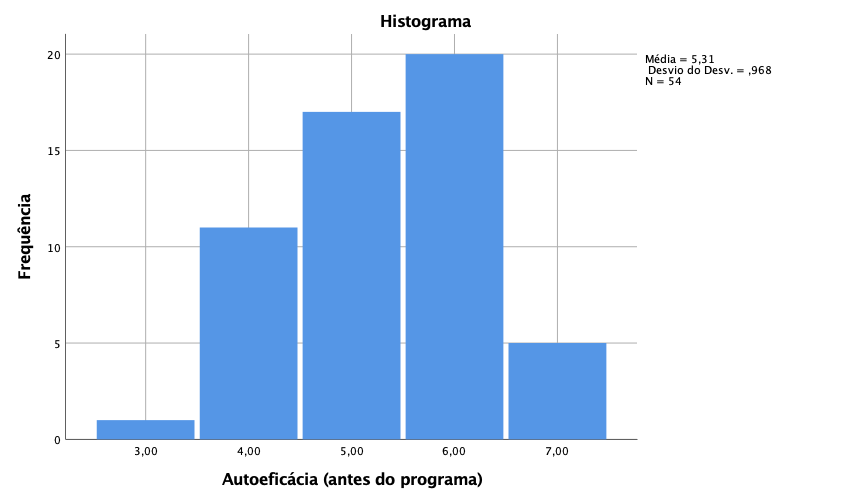
\includegraphics[scale=0.6]{Imagens/histograma_autoeficacia_antes.png}
\fonte{O autor}
\label{figura_29}
\end{figure}


Nas respostas por curso, os alunos do curso de zootécnica mostram-se mais seguros quando se compara as médias obtidas aos demais cursos participantes, saindo da média de 4,53 para 5,58. O curso apresentou um crescimento maior frequência na questão 5 \textit{um pouco seguro}, ouve um crescimento das respostas: 6 \textit{seguro} e 7 \textit{completamente seguro}, porém, os alunos que mostraram mobilidade na frequência da mediana foram os alunos matriculados no curso de engenharia agrícola, os quais saíram da questão 5 \textit{um pouco seguro} para 6 \textit{seguro}. Os alunos do curso de engenharia agronômica, passaram a se sentirem menos indecisos, mobilizando suas opiniões para as questões acima desta. O curso de engenharia de pesca não apresentou inscritos suficiente para manter uma frequência experimentável. Na figura \ref{figura_34} é possível observar a mobilidade das respostas dos alunos (aqui representado pelos quartis) após a participação no programa


\begin{figure}[H]
\centering
\caption{\textbf{Mobilidade de respostas sobre autoeficácia por curso}}
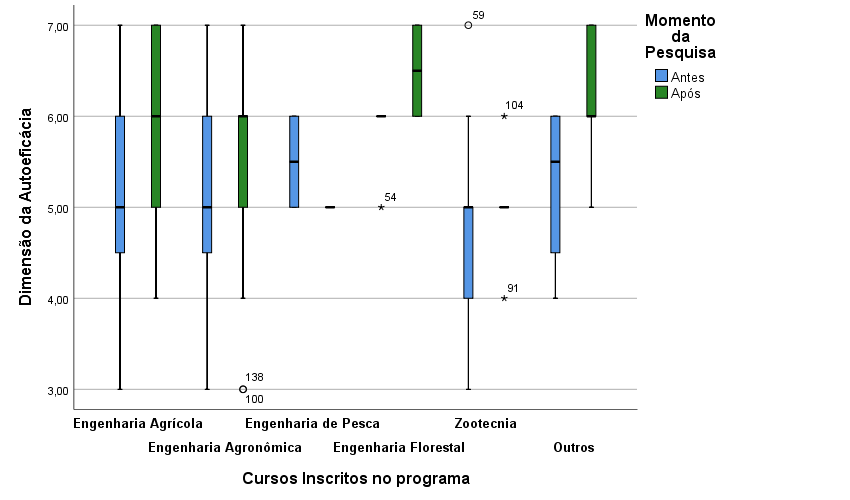
\includegraphics[scale=0.6]{Imagens/boxplot_autoeficacia.png}
\fonte{Autoria própria}
\label{figura_34}
\end{figure}


No Apêndice \ref{tab:amostras_autoeficacia} (Tabela \ref{tabela_5}), nota-se que as questões \textbf{Fazer análises financeiras"}, \textbf{"Reduzir riscos e incertezas"}, \textbf{"Assumir riscos calculados"}, \textbf{"Administrar o tempo estabelecendo metas"} e \textbf{"Conduzir minha própria empresa ao sucesso"} obtiveram valores de 0,007, 0,00, 0,024, 0,027 e 0,028 respectivamente, tais valores foram menores que o intervalo de confiança (0,05), podendo para estas questões ser rejeitado o H0 para a dimensão da autoeficácia . 


O fato de o programa Empreenda agro sustentável ter um caráter de pré-aceleração, foi pensado com o objetivo suprir uma lacuna na formação dos discentes das ciências agrárias e demais áreas da Universidade Federal de Sergipe, em relação ao desenvolvimento de um pensamento empreendedor, por meio da promoção de um ciclo de oficinas, visando a disseminação dos valores e técnicas dos gerenciamentos ágeis e a promoção do empreendedorismo capaz de aplicar tais metodologias na produção rural, pode ter influenciado na melhoria da autoeficácia para análise financeira dos negócios, a predição de riscos e possíveis mitigações, a gestão ágil do tempo e atividades relacionadas a inovação, e a promoção da disposição a assumir riscos calculados em novos empreendimentos. 

Tais resultados se aproximam com os observados por \citeonline{schafer_be_2018} sobre a mudança na autoeficácia para o empreendedorismo social, investigando as necessidades motivacionais que influenciam a intenção de potenciais empreendedores, observou que a educação para o empreendedorismo no promove a melhoria da autoeficácia empresarial, e que a desejabilidade de criar novos negócios para o âmbito social, foi determinada pela vontade dos alunos de auto realização e autonomia pessoal, após a vivência de conteúdos voltado a educação empreendedora. 

Neste sentido, levando em consideração os resultados da dimensão autoeficácia observada no estudo, não se rejeita a hipótese nula (H0) (Não há diferença entre as médias das medidas que averíguam o perfil empreendedor entre os alunos participantes do Programa de extensão Empreenda Agro Sustentável), quando observado os resultados da diferença apresentada no teste estatístico, contudo o programa empreenda agro sustentável proporciono uma mobilização positiva das respostas quando se comparado aos resultados iniciais dos participantes.


\subsection{Dimensão e intenção ao empreendedorismo dos estudantes}

A IE pode ser definida como uma intenção pessoal conduzida por ações e objetivos futuros a ser implementadas buscando o desenvolvimento de novos empreendimentos. A IE é uma função das características do nível individual e dos contextos acadêmicos e sociais, com algum grau de efeitos específicos durante a vida acadêmica, desta forma diversificar os conteúdos dos futuros profissionais é uma questão crítica que merece atenção da comunidade de ensino de engenharia \cite{gilmartin_entrepreneurial_2019}.

É sabido que a IE antecede o passo de criação do negócio, embora nem sempre é o principal componente para surgimento de novos negócios, restrições financeiras e falta de informação e a capacidade de acumular capital específico (que é aprendido com parentes que eram empreendedores), podem ser fatores que interfiram na abertura de novos negócios mesmo que esteja presente a Intenção de empreender \cite{auguste_what_2016}.



\begin{figure}[H]
\centering
\caption{\textbf{Contagem Dimensão da Intenção empreendedora  por Momento da Pesquisa}}
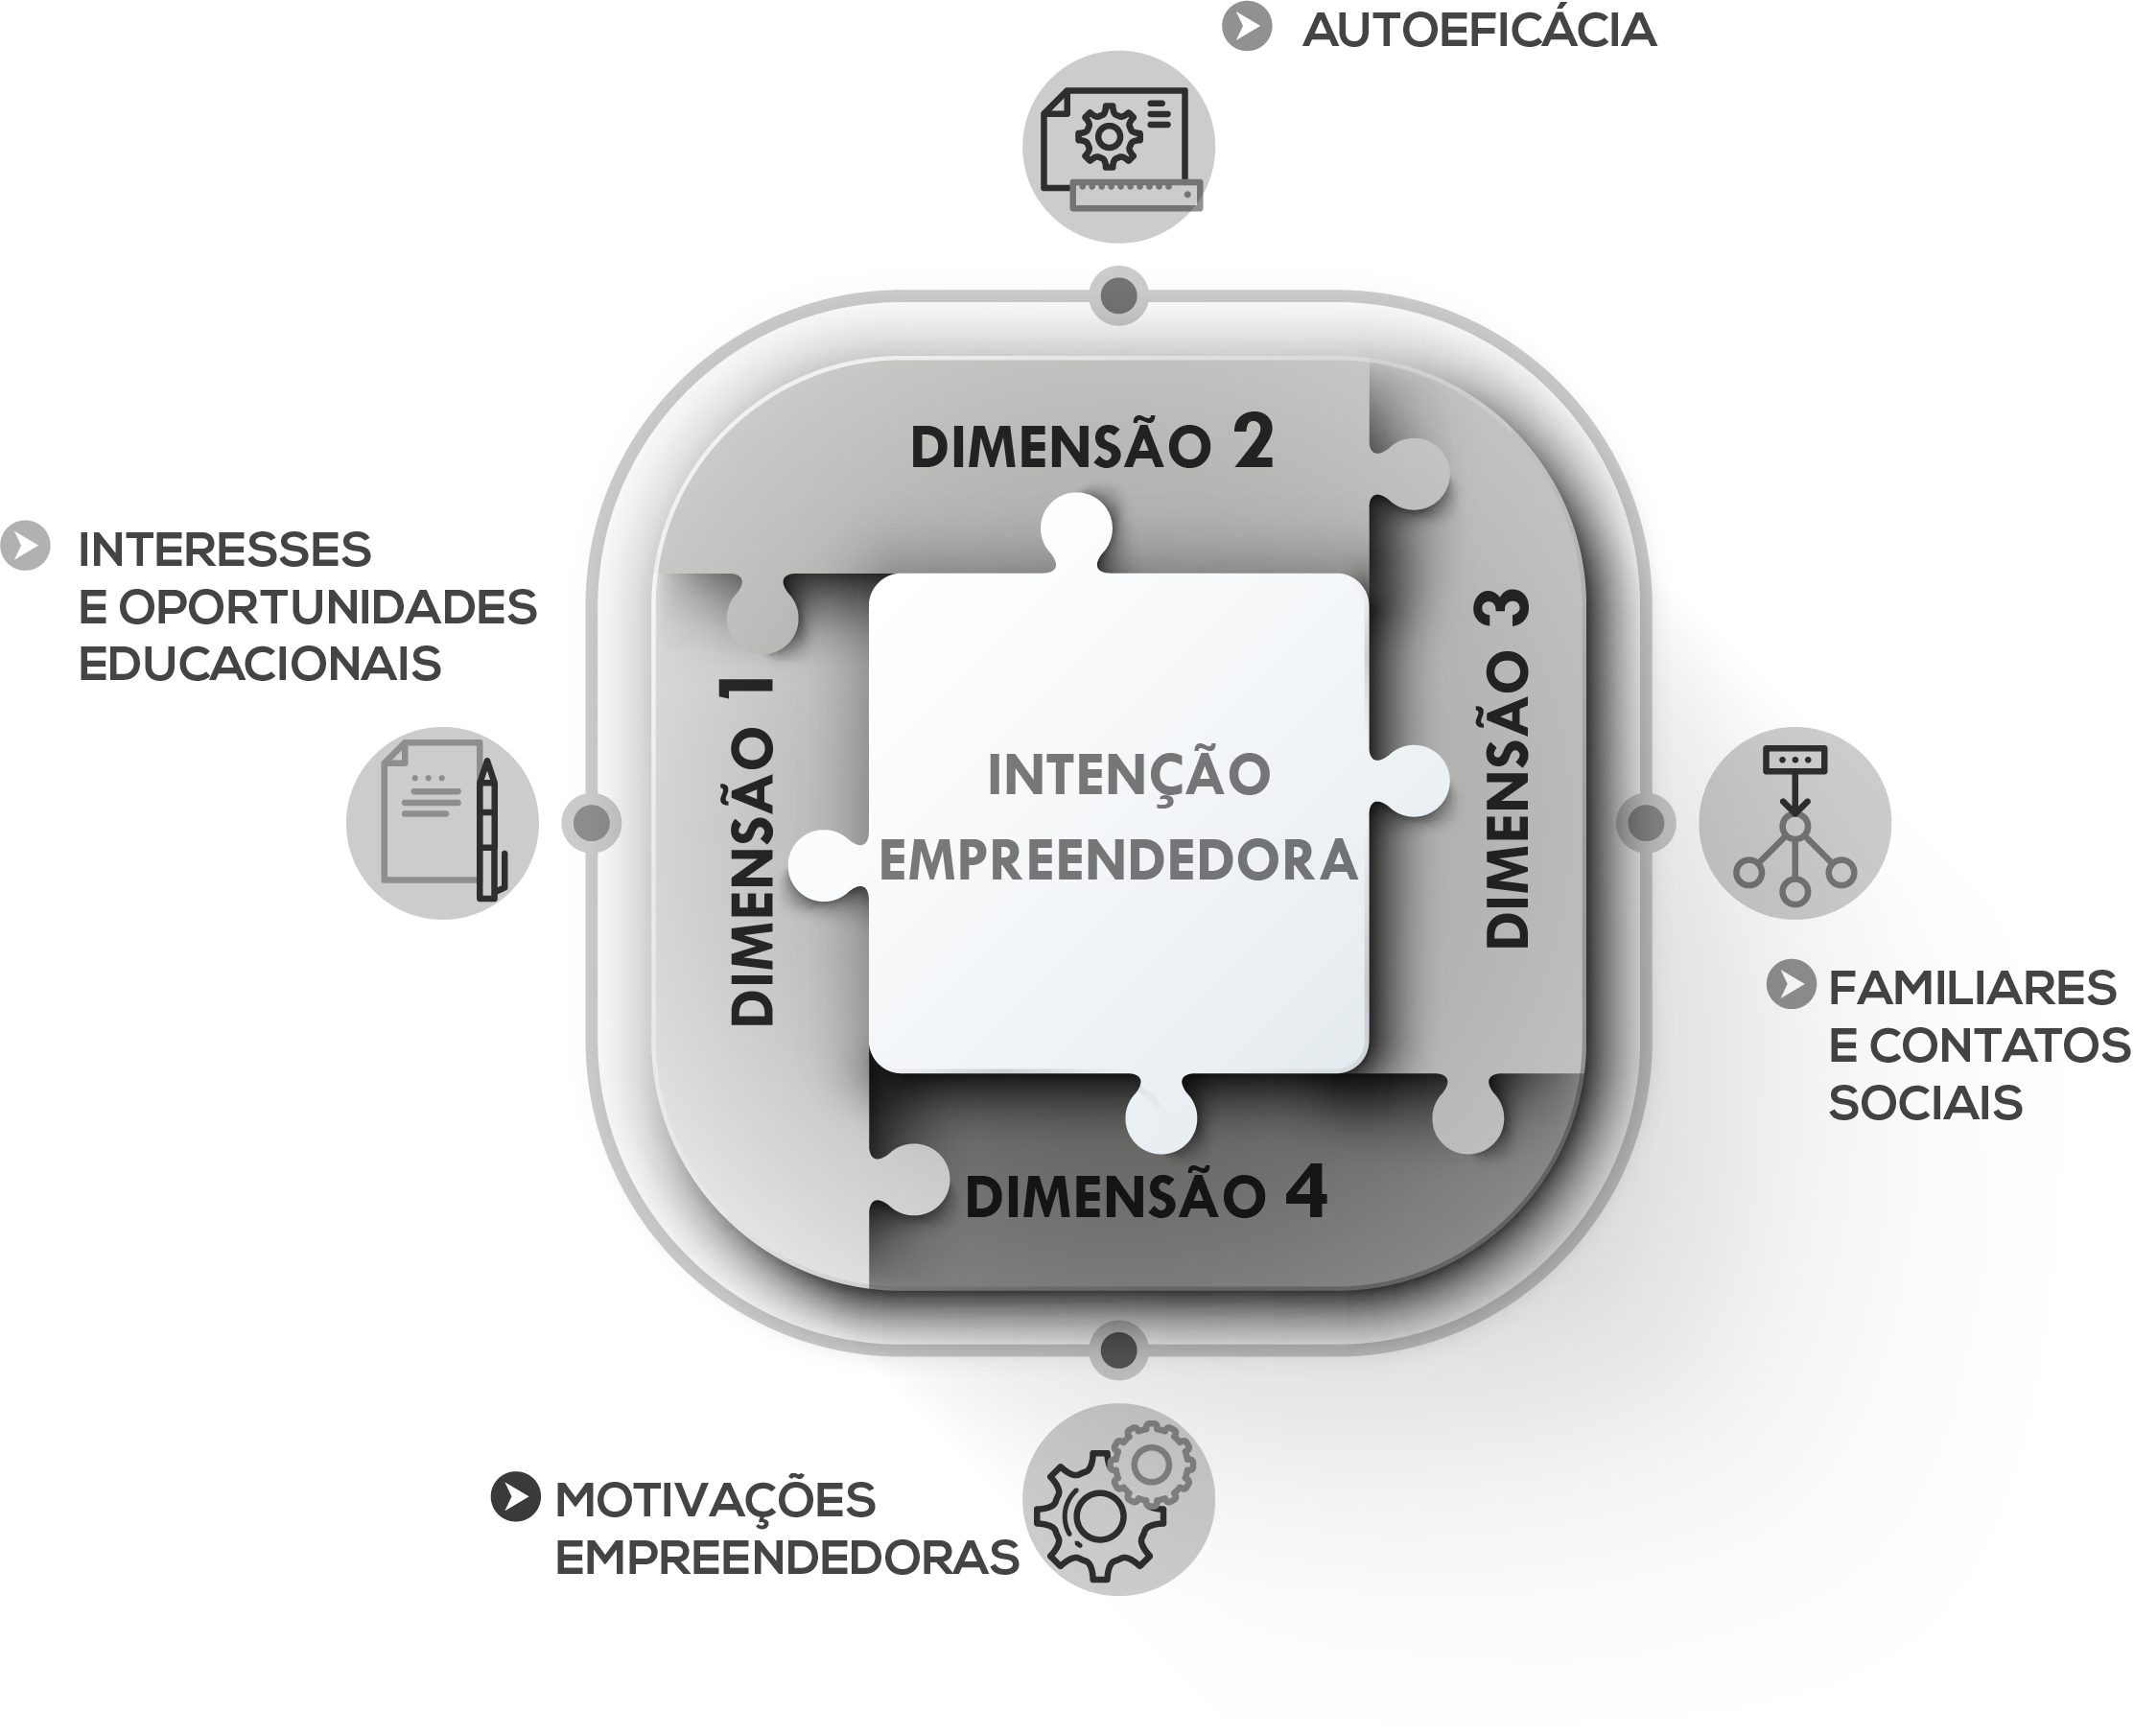
\includegraphics[scale=0.6]{Imagens/intencao_empreendedora.png}
\fonte{O autor}
\label{figura_45}
\end{figure}


\subsection{Dimensão da participação familiar e influência de terceiros no desenvolvimento empreendedorismo}



\section{Inovações desenvolvidas: Marcas}
\label{inovacoes}

O programa foi concluído  com a participação de 15 equipes (Aqua plant, Be Soluções, La Flora Pet, Agrion, Grão Nordestino, MAMP, AGROPEC, Horta House, Ranagro, Agro View, Itecagro, Tecno Coco, BAgrotec, Impacto Pescados, Uneagro), resultando ao final com 16 marcas, 15 para os grupos e a marca própria do programa, como mostrado  \ref{figura_12}.

%\begin{multicols}{3}
%\centering
%    \begin{itemize}
%\item {(a) Aqua plant;}
%\item {(b) Agrion;}
%\item {(c)AGROPEC;}
%\item {(d) Agro View;}
%\item {(e) BAgrotec;}
%\item {(f) Be Soluções;}
%\item {(g) Grão Nordestino;}
%\item {(h) Horta House;}
%\item {(i) Itecagro;}
%\item {(j) Impacto Pescados;}
%\item {(l) La Flora Pet;}
%\item {(m) MAMP;}
%\item {(n) Ranagro;}
%\item {(o) tecno Coco;}
%\item {(p) Uneagro;}
%\end{itemize}
%\end{multicols}



\begin{figure}[H]
\centering
\caption{\textbf{Portfólio das marcas desenvolvidas durante o programa}}
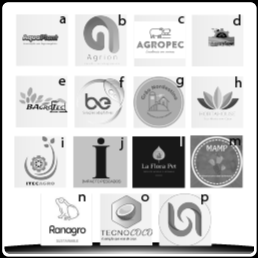
\includegraphics[scale=3]{Imagens/portfolio.png}
\fonte{O autor}
\label{figura_12}
\end{figure}


\subsection{Aqua plant}



A Startup visa justamente acabar com as incertezas que  afligem o agricultor quanto á sua produção, visto que nosso produto é um sistema de aquaponia fechado, com recirculação de água, ao qual no final do processo o produtor terá garantido proteína e hortaliças de qualidade. 

Venderemos nosso produto, que irá integrado em pacotes de assistência técnica, tanto diretamente ao produtor como também em contratos com municípios. Nossa equipe é formada por 3 estudantes de Engenharia Agronômica e 2 Engenheiros de pesca, e por meio desse ciclo a AquaPlant irá fazer produzir no Sertão (Figura \ref{figura_13}).


\begin{figure}[H]
\centering
\caption{\textbf{Marca Aquaplant}}
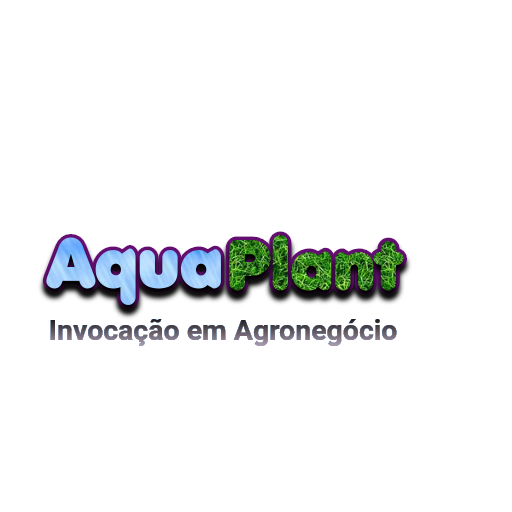
\includegraphics[scale=0.4]{Imagens/aquaplant.png}
\fonte{\cite{ufs_empreenda_2019}}
\label{figura_13}
\end{figure}


\subsection{Agrion}

Aplicativo desenvolvido por sistemas digitais afim de conectar diretamente os aplicativos desenvolvido para sistemas produtores aos mercados varejistas no processo de compra e venda de produtos agrícolas onde a lucratividade é prevista por meio da cobrança de taxação em cima do montante total de vendas diferenciando valores de venda em atacado e varejo, e porcentagem por tipo de produto.

O grande número de produtores agrícolas  do mercado sergipano com relativo que  em sua grande maioria são oriundos da agricultura familiar e ao mesmo tempo um contingente potencial de consumidores em uma curta distância. Isso baseado na  participação das cooperativas desses produtos que de acordo 
com federação tem mais de 75 cooperados e que, as mesmas têm demostrado ter capacidade de suprir o aumento da demanda (Figura \ref{figura_14}).


\begin{figure}[H]
\centering
\caption{\textbf{Marca Agrion}}

\includegraphics[scale=0.2]{Imagens/agrion.png}
\fonte{\cite{ufs_empreenda_2019}}
\label{figura_14}
\end{figure}

\subsection{BAgrotec}

Com o App TecAgro iremos conectar o produtor ao profissional, solucionando problemas no campo e consequentemente, gerando mercado de trabalho para os profissionais. Além do app o site da BAgroTec irá auxiliar no cadastramento de produtores que tiverem dificuldades com a plataforma mobile.  

O aplicativo irá valorizar o profissional gerando currículo dentro da plataforma  produtor terá acesso e retorno Imediato do profissional. Irá e fornecerá dados que irá auxiliar o profissional na tomada de decisão no campo

Muito mais que ofertar serviços de assistência técnica estamos ofertando qualidade na produção e mudaremos o atual cenário da desvalorização do profissional das agrárias(Figura \ref{figura_15}).

\begin{figure}[H]
\centering
\caption{\textbf{Marca BAgrotec}}

\includegraphics[scale=1.0]{Imagens/bagrotec.png}
\fonte{\cite{ufs_empreenda_2019}}
\label{figura_15}
\end{figure}


\subsection{AGROPEC}


A proposta da Startup, é aproximar a indústria frigorifica dos  produtores rurais, gerindo os rebanhos, administrando um 
confinamento coletivo, comercializando animais terminados para os frigoríficos e vendendo matrizes e reprodutores em plataformas de vendas online. Iniciaremos o trabalho com 10 fazendas e um rebanho geral de 1000 matrizes, sendo planejado triplicar o rebanho atendido até o final do sétimo ano e faturar anualmente pouco mais de dois milhões de reais.

O modelo de negócio está baseado na produção de carne de  cordeiro com eficiência zootécnica e na gestão financeira, além 
da bonificação dos resultados, compra e venda de produtos  agrícolas onde a lucratividade é prevista por meio da cobrança de taxação em cima do montante total de vendas diferenciando valores de venda em atacado e varejo, e porcentagem por tipo de produto (Figura \ref{figura_18}).


\begin{figure}[H]
\centering
\caption{\textbf{Marca AGROPEC}}

\includegraphics[scale=0.2]{Imagens/agropec.jpg}
\fonte{\cite{ufs_empreenda_2019}}
\label{figura_18}
\end{figure}

\subsection{Agro View}


Os Agroview, para terem um monitoramento mais intensivo da  produção terão que fazer um contrato mensal com a 
sua lavoura, afim de ser mais assertivo na identificação e tomada de decisão de aplicar os produtos  na hora certa, controlando antes que as pragas possam causar danos severos a lavoura, e assim  evitando uso desnecessário dos agrotóxicos. O controle quando necessário, será realizado com o uso de um drone, para dar mais agilidade ao processo e eficiência principalmente em local de difícil acesso, onde pessoas e até máquinas conseguiriam chegar, caso  de áreas muito declivosas. Essa empresa é composta por três engenheiros Agrônomos e um Engenheiro Agrícola, preparados para fazer controle biológico, seguindo  essa  visão sustentável que  já é uma tendência global. Temos um mercado gigante e promissor a ser  conquistado não só no Brasil, mas também no mundo inteiro.

Onde a startup irá disponibilizar todos os nossos serviços e  osso modelo de negócio é baseado em assinaturas mensais assistência técnica ao produtor rural. E também contratos emergenciais. Ademais, nosso cliente pode entrar em contando por meio de telefone celular e redes sociais (Figura \ref{figura_19}).


\begin{figure}[!htb]
\centering
\caption{\textbf{Marca Agro View}}

\includegraphics[scale=0.2]{Imagens/agroview.jpg}
\fonte{\cite{ufs_empreenda_2019}}
\label{figura_19}
\end{figure}


\subsection{Be Soluções}

No atual cenário global, há cada vez uma maior demanda por métodos produtivos mais sustentáveis, especialmente quando relacionados a recursos hídricos. De acordo com a Agência Nacional de Águas (ANA), o Brasil está entre os dez países com a maior área irrigada, com cerca de 6,95 milhões de hectares (Mha), que produzem alimentos utilizando diferentes técnicas de irrigação. Segundo o Sistema Nacional de Informações sobre o Saneamento (SNIS), calcula-se que no Brasil o consumo médio de água é de 10,4 trilhões de litros ao ano, onde deste total, pouco mais de 7 trilhões são destinados à agricultura, e que deste 7 trilhões destinado a este setor, aproximadamente 3 trilhões são desperdiçados devido ao mau uso.

Para reduzir essa problemática propomos a utilização de um sistema. Um pacote tecnológico com sensores instalados em campo, que coletam dados importantes como: umidade, temperatura e condutividade elétrica, tudo em tempo real, que serão transmitidos sem fio para uma central eletrônica para um controle preciso do sistema
de irrigação, permitindo o uso mais eficiente e sustentável dos recursos hídricos.

Para reduzir essa problemática propomos a utilização de um sistema. Um pacote tecnológico com sensores instalados em campo, que coletam dados importantes como: umidade, temperatura e condutividade elétrica, tudo em tempo real, que serão transmitidos sem fio para uma central eletrônica para um controle preciso do sistema de irrigação, permitindo o uso mais eficiente e sustentável dos recursos hídricos.

Diferente dos sistemas atuais que possuem um alto custo e que não apresentam tantos recursos de forma unificada em um só equipamento, buscamos desenvolver um produto que proporcione uma alta precisão ao utilizar um sistema de dados coletados em tempo real, obtidos no local especifico da cultura. Esse equipamento é adaptativo as diferentes culturas e tipos de solo. Através de uma simples configuração na central eletrônica, por meio de uma de tela \textbf{touch} e interface intuitiva, é possível realizar uma irrigação precisa com somente a quantidade de água que a cultura selecionada necessite (Figura \ref{figura_20}).

\begin{figure}[!htb]
\centering
\caption{\textbf{Marca Be Soluções}}
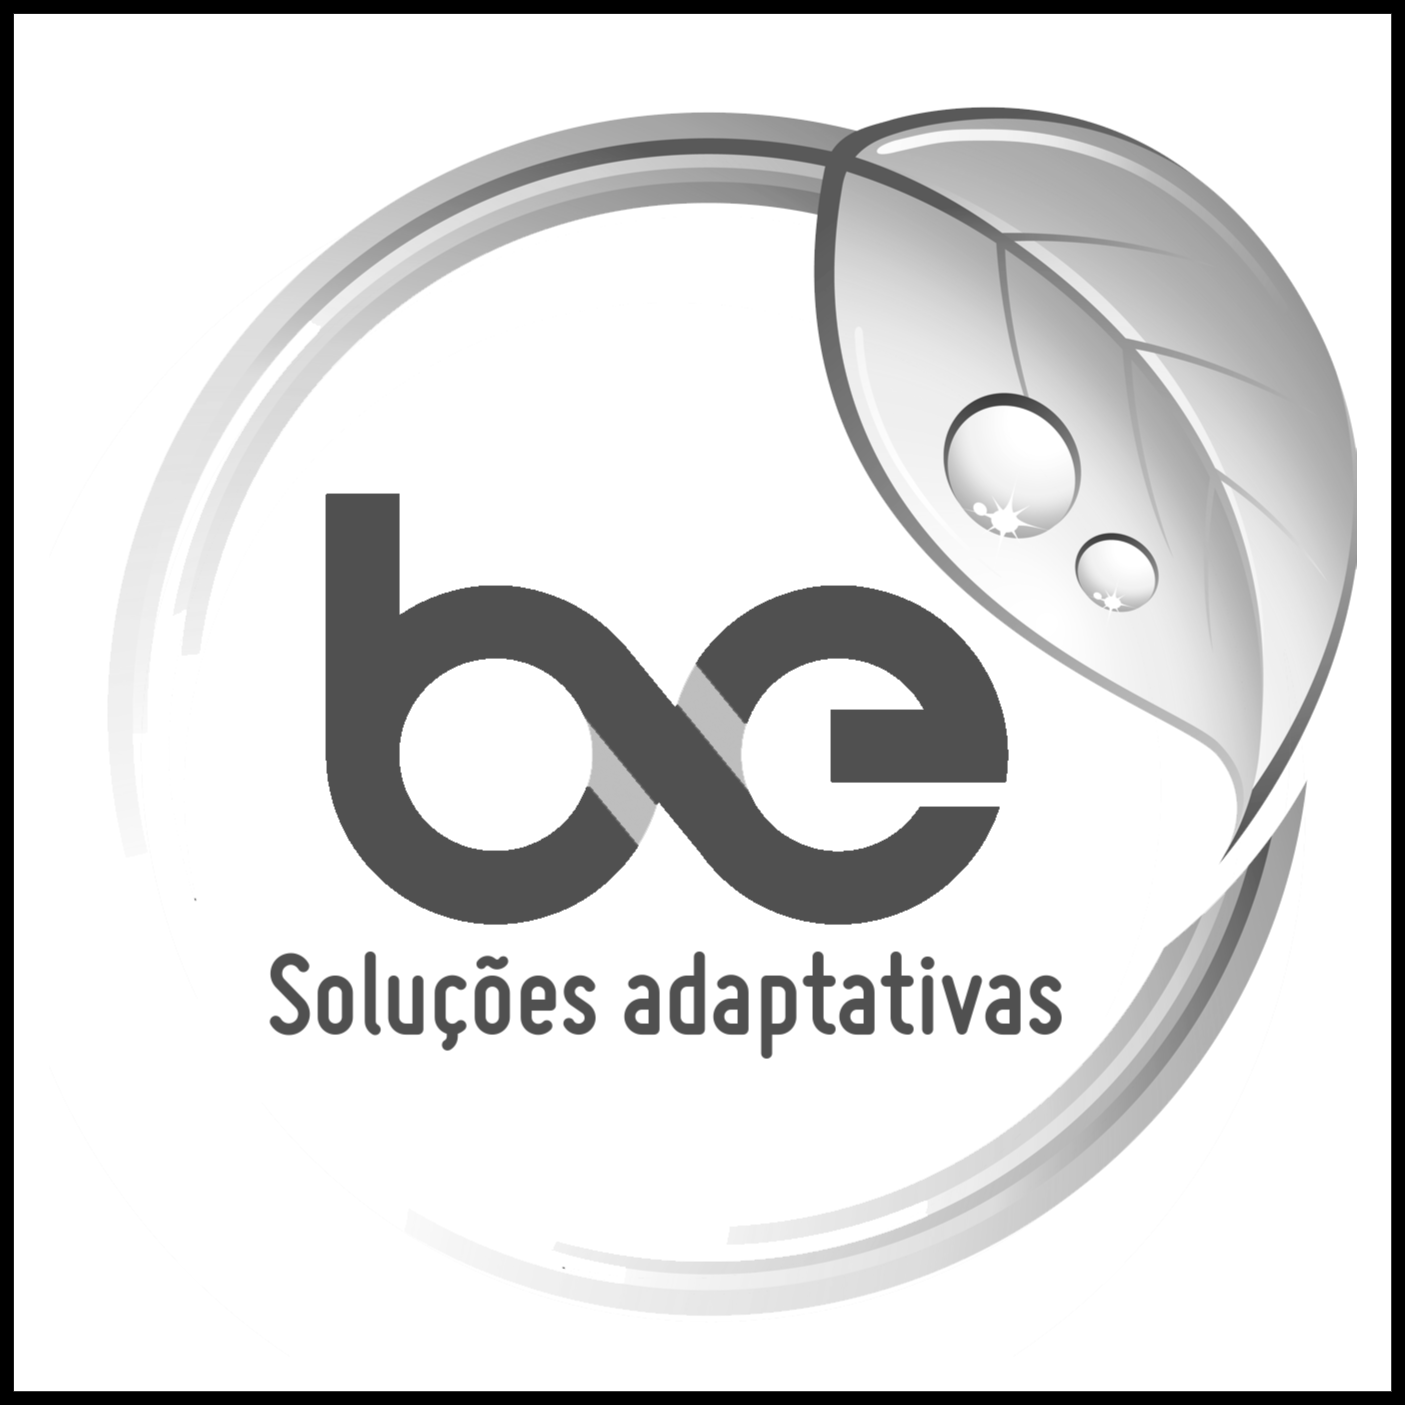
\includegraphics[scale=0.4]{Imagens/besolucoes.png}
\fonte{\cite{ufs_empreenda_2019}}
\label{figura_20}
\end{figure}




\subsection{Grão Nordestino}

Conhecendo a realidade do pequeno e médio produtor que por falta de uma unidade armazenadora perdem boa parte da sua colheita ou são obrigados a vender com o menor preço para que não venha a perder seu produto, nós da grão Nordestino trazemos o que vem a ser a solução para esse problema, projetando e instalando silos de baixo custo e sustentáveis, agregando valor ao seu produto e combatendo o desperdício de alimentos mal armazenados.

O produtor terá acesso e retorno Imediato do profissional, irá valorizar o profissional gerando currículo dentro da plataforma e fornecerá dados que irá auxiliar o profissional na tomada de decisão no campo (Figura \ref{figura_21}).


\begin{figure}[H]
\centering
\caption{\textbf{Marca Grão Nordestino}}
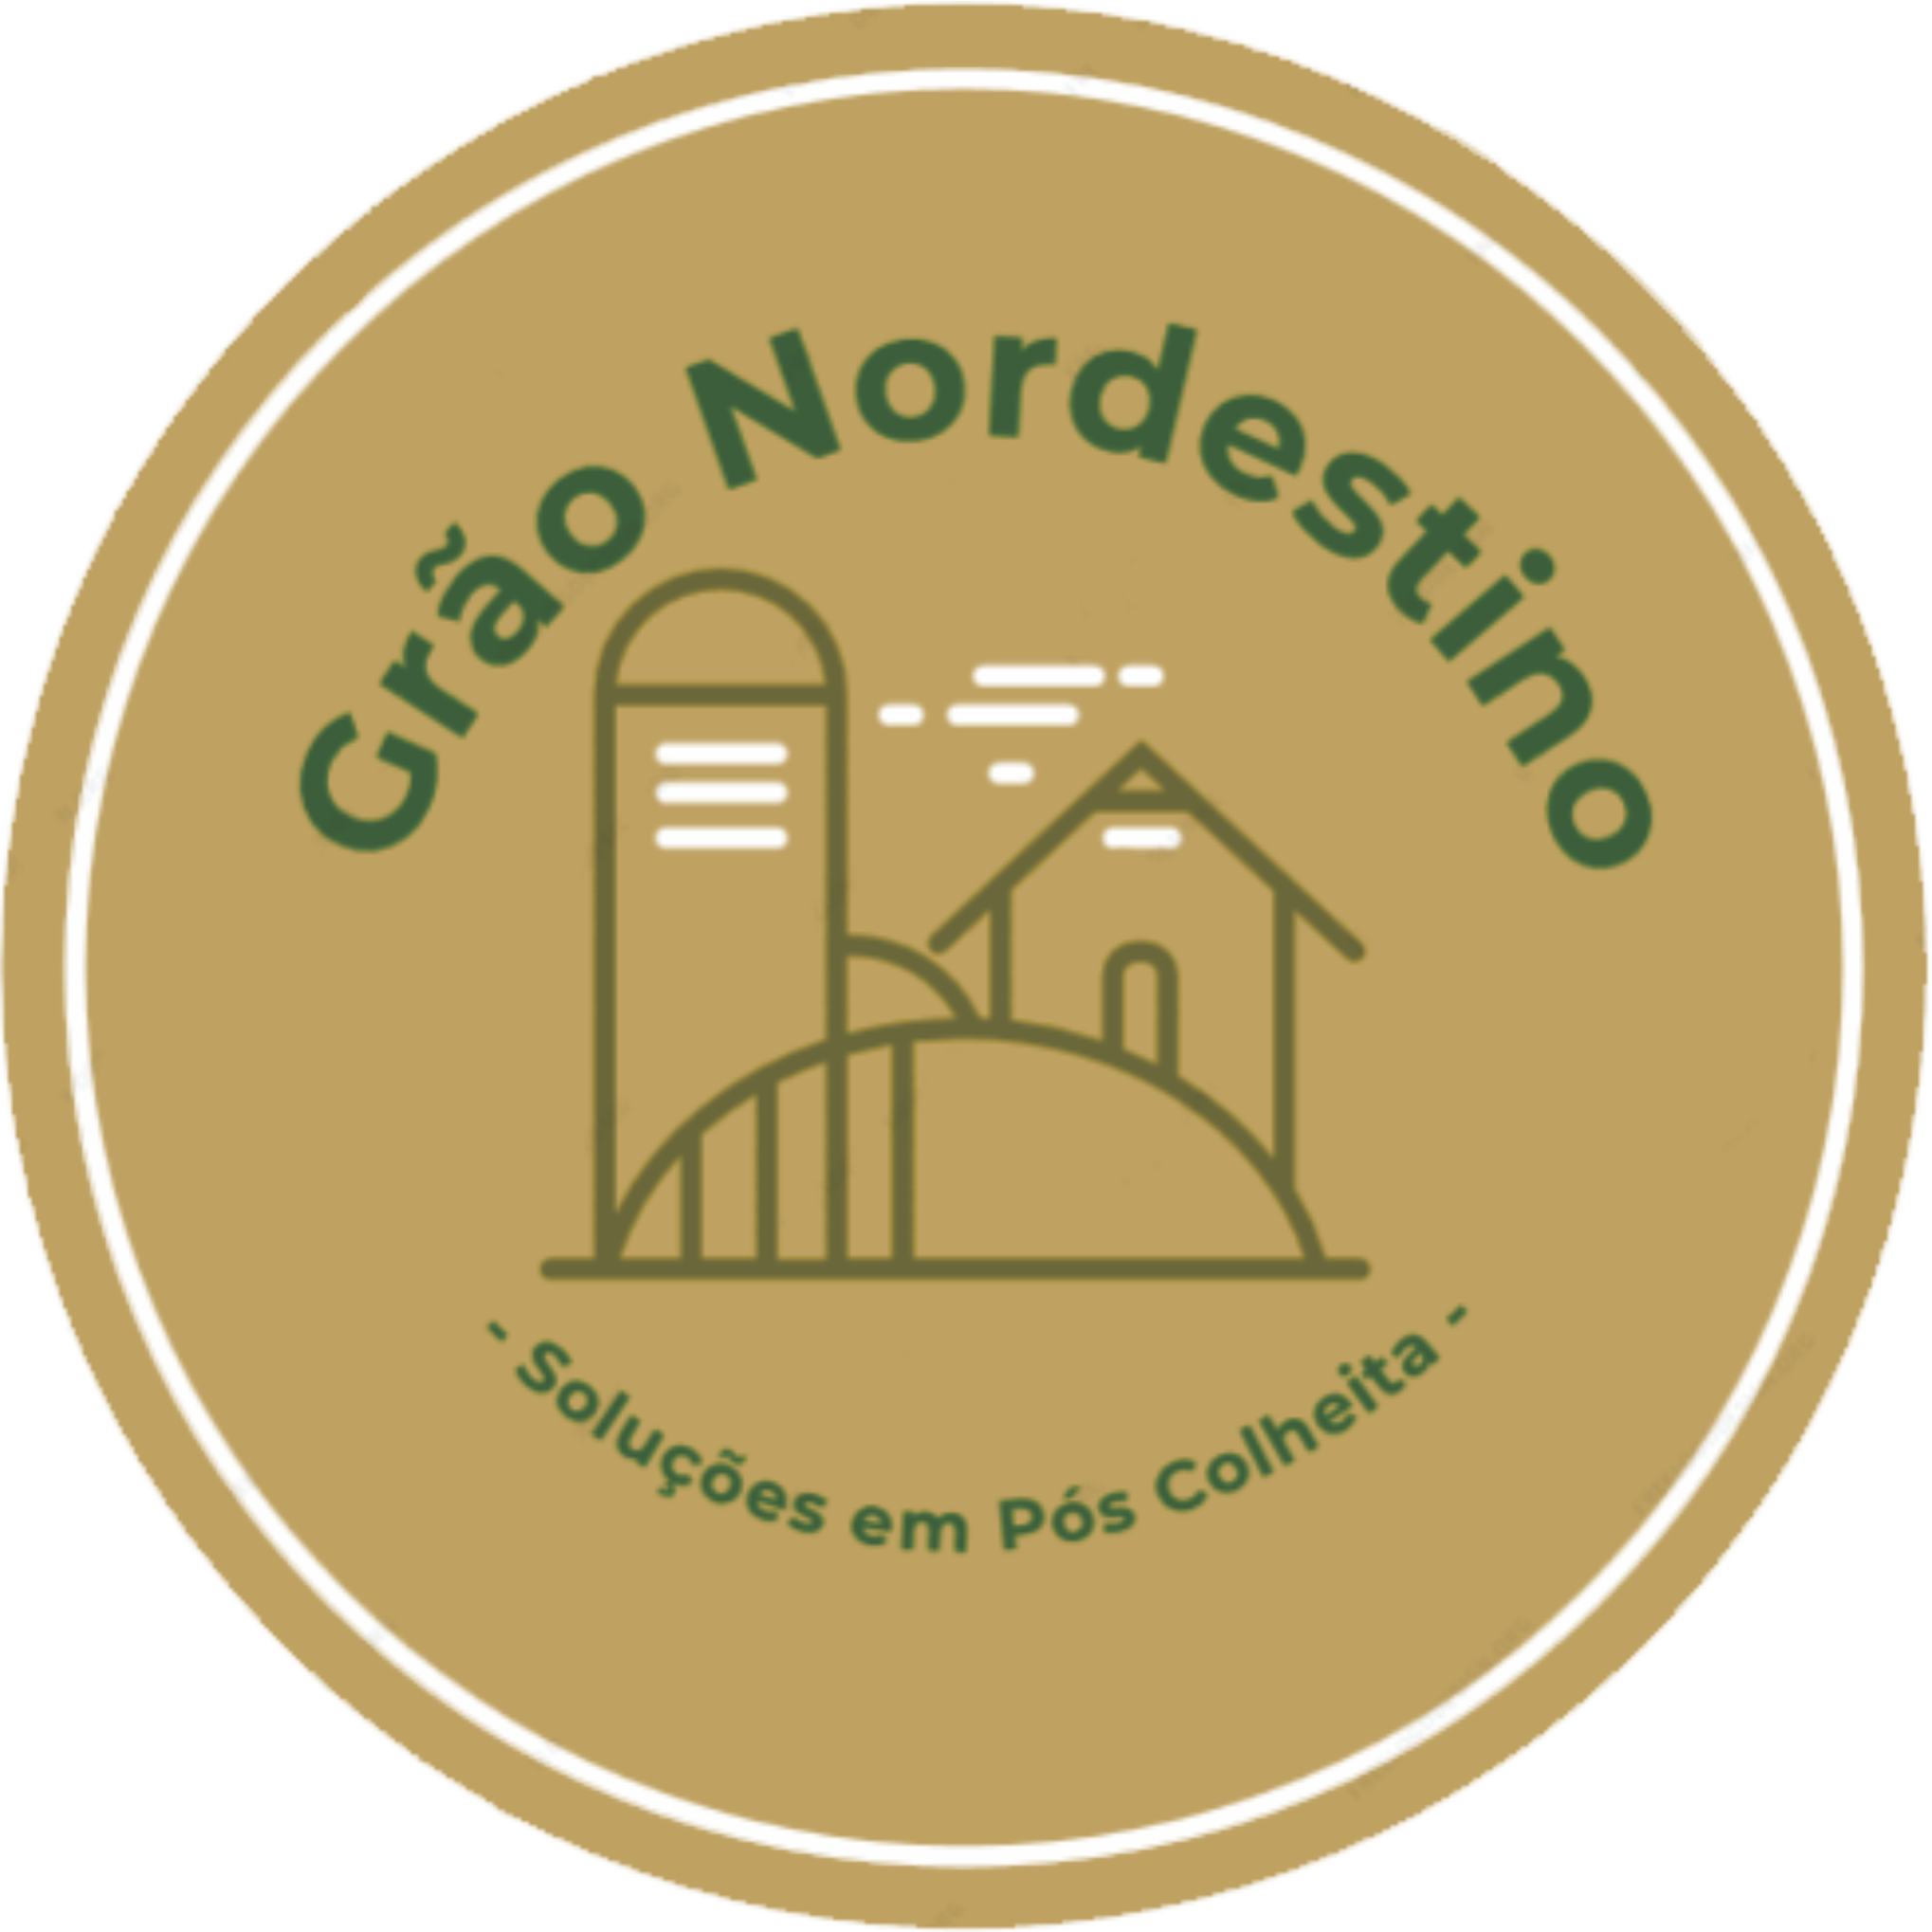
\includegraphics[scale=0.3]{Imagens/graonordestino.png}
\fonte{\cite{ufs_empreenda_2019}}
\label{figura_21}
\end{figure}



\subsection{Horta House}


O número de empresas especializadas em consultoria para hortas urbanas ainda é insuficiente para atender essa demanda que continua a crescer, tentando solucionar esse problema muitas pessoas recorrem a ferramentas de busca na internet e acabam tomando como base instruções de pessoas que muitas vezes não possuem uma qualificação para recomendações técnicas, o que em alguns casos acaba fazendo com que as plantas cultivadas entrem em um processo inverso ao desejado, ou seja morrem,

Visando solucionar esses problemas nossa empresa pretende fornecer consultoria técnica de qualidade, tendo em vista que nossa equipe é formada por três engenheiros agrônomos. Junto a nossa
consultoria pretendemos ofertar a construção de hortas planejadas de forma a que as mesmas se adéquem as necessidades do cliente, sendo incluído nesse planejamento o fornecimento de substrato, soluções nutritivas e adubos orgânicos, além das mudas (Figura \ref{figura_25}).


\begin{figure}[H]
\centering
\caption{\textbf{Marca Horta House}}
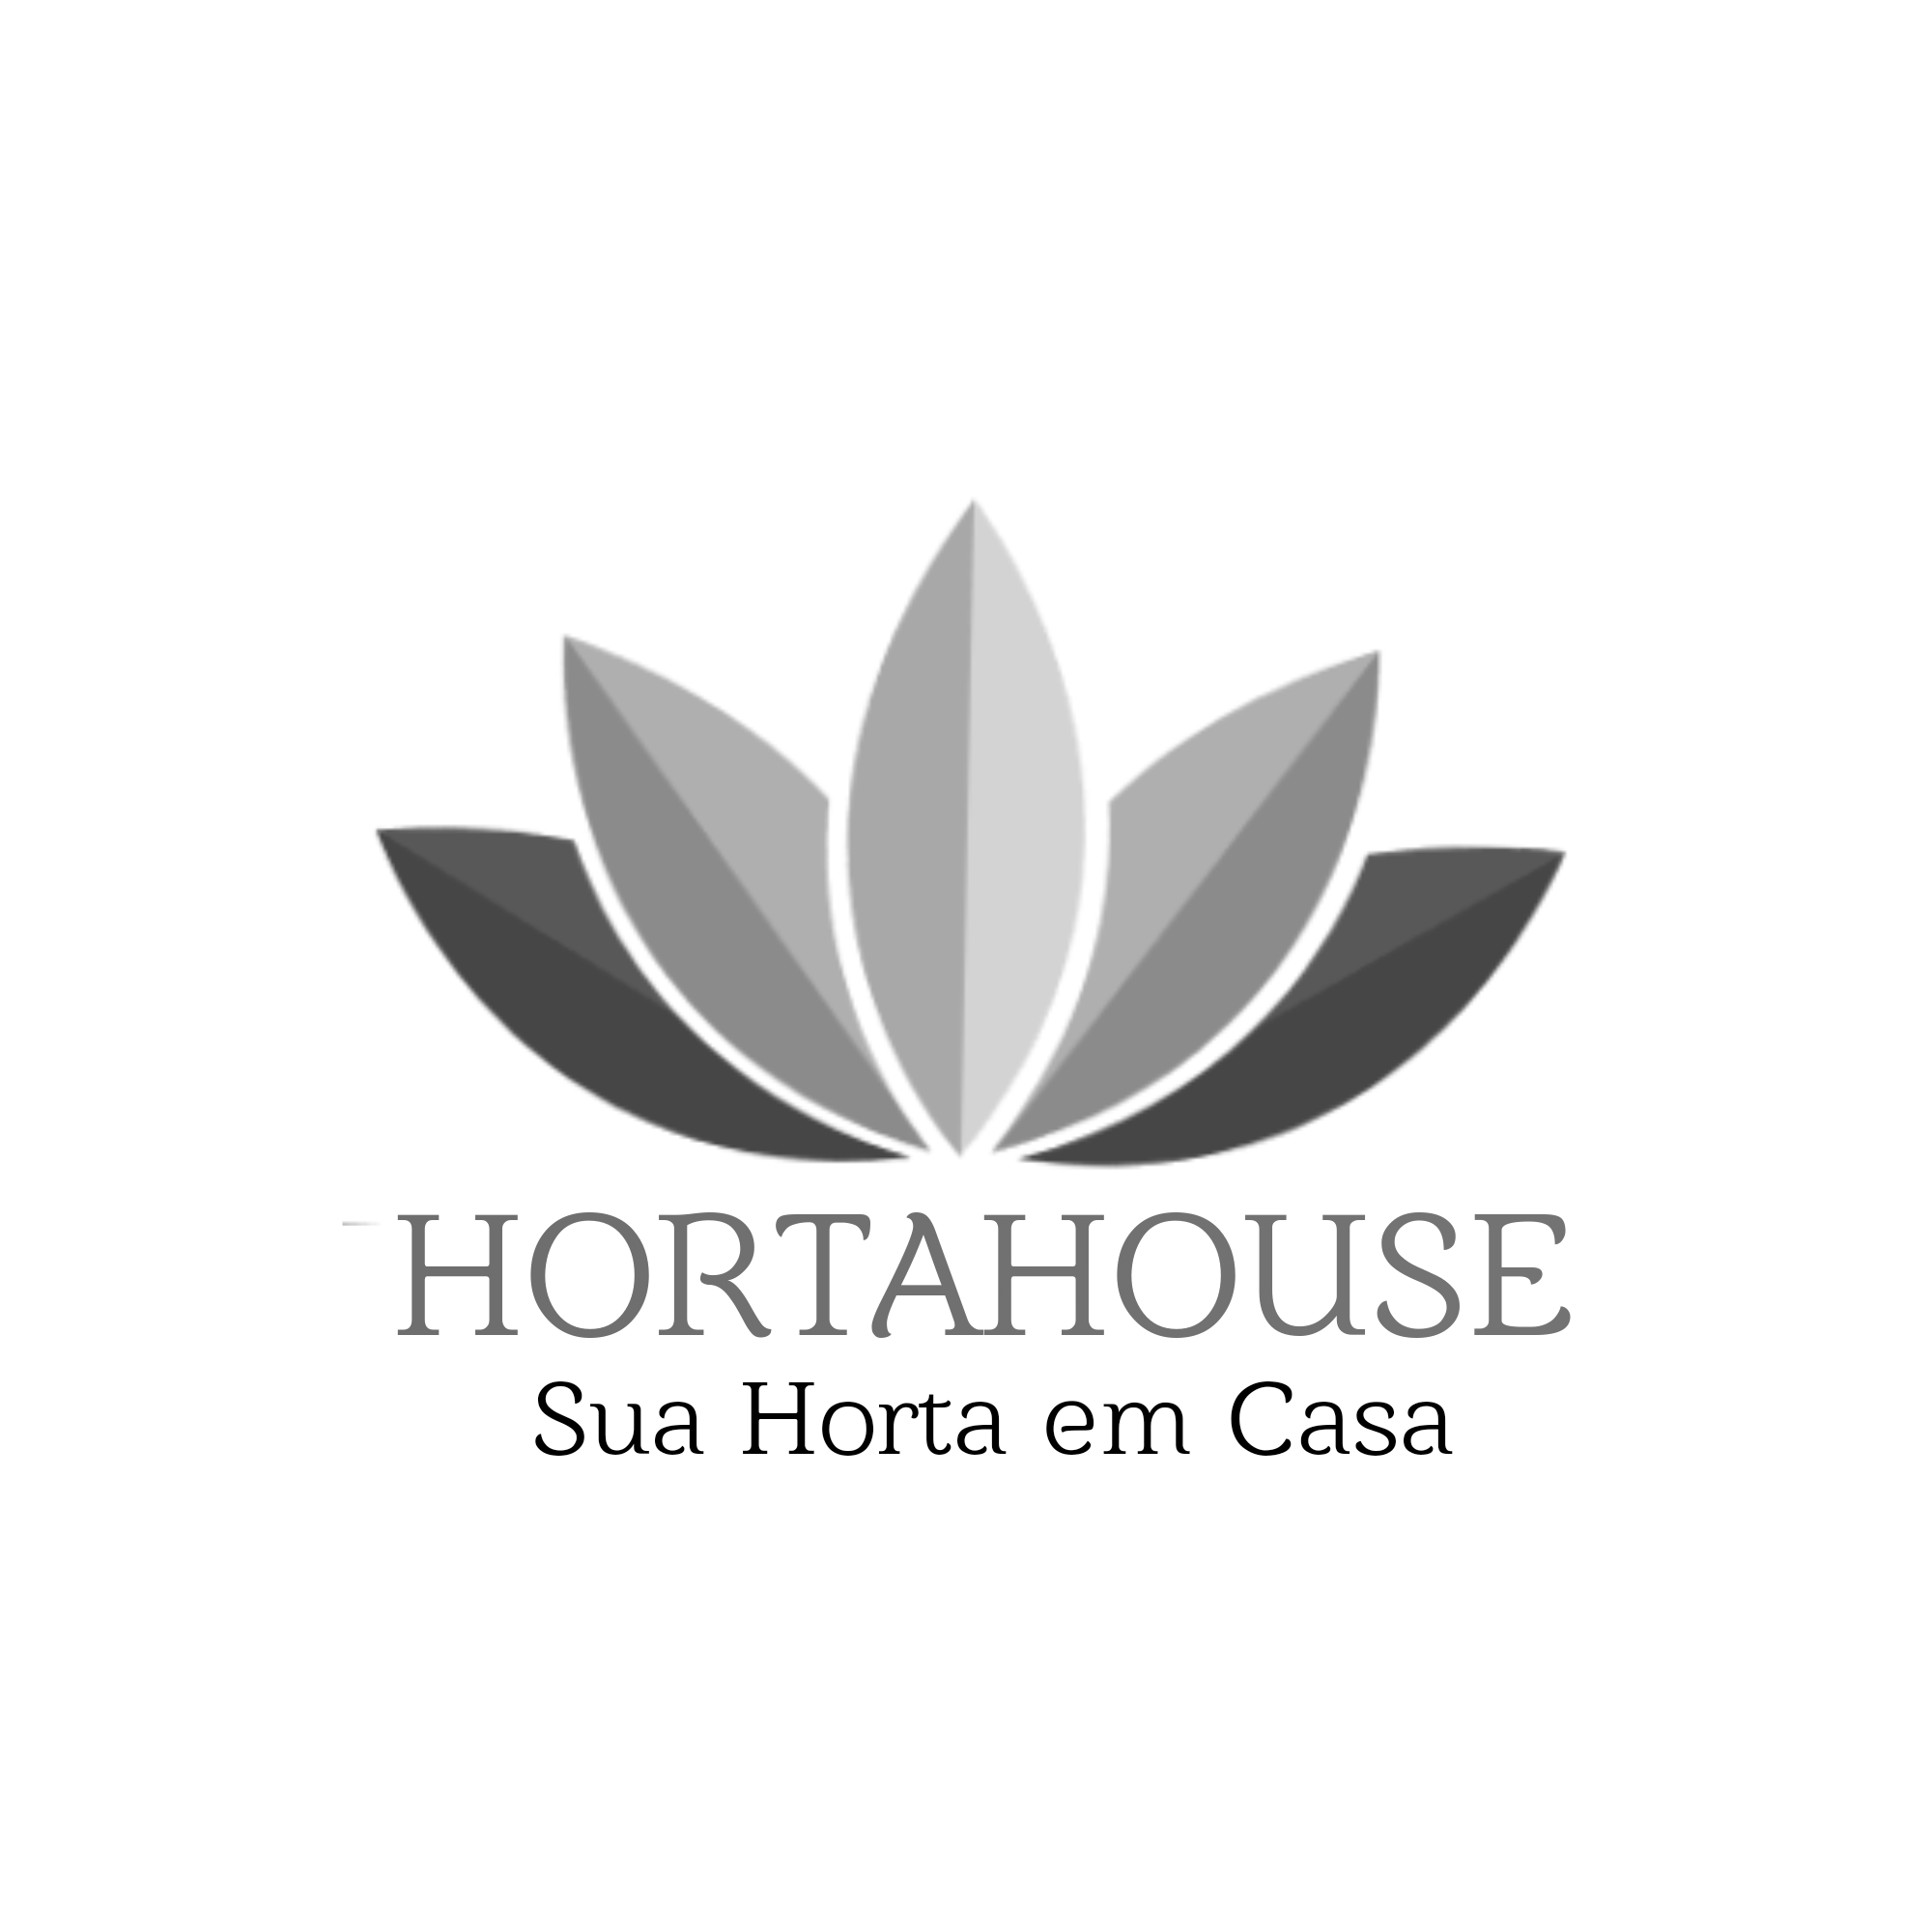
\includegraphics[scale=0.1]{Imagens/hortahouse.png}
\fonte{\cite{ufs_empreenda_2019}}
\label{figura_25}
\end{figure}



\subsection{ItecAgro}

Plataforma de interação direta com uma equipe multidisciplinar voltada
para o agro, que se utiliza de sistemas digitais para dinamizar seu negócio de forma: Inovadora, Empreendedora e Sustentável; Propor um canal facilitador, através de sistemas digitais para dinamizar o negócio da agricultura de forma inovadora, empreendedora, e sustentável.
Tem a visão de Ser uma startup de referência desenvolvendo soluções através da assistência técnica de qualidade gerando valor ao produtor e promovendo responsabilidade socioambiental, e trabalho com excelência.
Seguindo os valores de: Inovação, Humanização, Sustentabilidade, Ética, Transparência, Profissionalismo, Confiabilidade e Tecnologia (Figura \ref{figura_46}).

\begin{figure}[!htb]
\centering
\caption{\textbf{Marca Itec Agro}}

\includegraphics[scale=0.1]{Imagens/itecagro.png}
\fonte{\cite{ufs_empreenda_2019}}
\label{figura_46}
\end{figure}
\newpage


\subsection{Impacto Pescados}

Empresa especializada na criação de camarão do tipo \textit{Litopenaeus vannamei} com a utilização de bomba movida a óleo diesel para sucção da água do mar viabilizando as trocas de água com uma maior frequência tornando o menor tempo de cultura lançando no mercado um produto de qualidade com um menor período de cultivo. Em outras palavras baixamos o tempo de cultivo para 30 dias. A despesca do camarão de 10 gramas. O cultivo pesquisado num criador comum, foram necessários 70 dias para mesma gramatura. Custa-se, dessa forma, 5,00 R\$kg do camarão cinza. Podendo, assim, vender o produto a 15,0 0R\$ no mínimo. Segundo a Embrapa a pesca mundial não supre a demanda por pescados, ou seja, há um problema no equilíbrio entre a oferta e a demanda. Além disso, existe o fato do preço elevado para o camarão. Sendo assim, soluciona-se esta problemática com criação de camarão em viveiros além de fazê-lo com o menor preço e melhor atendimento.

Visto isso, nota-se que nosso lucro gira em torno de 200\% a cada 30 dias no Máximo, o qual é no modo monofásico-quando com apenas um tanque, você faz as fases: pré-berçário, berçário e engorda. Aliado a isso podemos fazer no modo trifásico conforme o capital disponível para custear três tanques pra fazer as três fases e diminuir a 11 dias a despesca (Figura \ref{figura_23}).

\begin{figure}[H]
\centering
\caption{\textbf{Marca Impacto Pescados}}

\includegraphics[scale=0.4]{Imagens/imacto_pescados.jpg}
\fonte{\cite{ufs_empreenda_2019}}
\label{figura_23}
\end{figure}


\subsection{La Flora Pet}

Observando o crescimento do mercado PET nos últimos anos e a persistência nas dores sofridas pelos donos desses animais com relação a custo alto e acessibilidade a tratamentos eficientes, a La Flora Pet desenvolve produtos naturais e artesanais com base em extratos ou óleos essenciais cujo objetivo é prevenir ou tratar distúrbios comportamentais e dermatológicos em cães e gatos ofertando produtos de baixo custo

Sabendo das limitações variadas de cada espécie, raça, idade e sexo do animal, nossos profissionais são capacitados a atender de forma intimista a necessidade do usuário sem causar transtornos toxicológicos e agindo de forma eficiente no tratamento ou prevenção de doenças. La Flora Pet a magia da natureza a um clique de distância.

Nosso plano de negócio é a venda desses produtos, que através do site da loja será personalizado pelo próprio cliente. Após cadastramento de dados pessoais do cliente e usuário, a personalização consiste em escolher o extrato ou óleo essencial de acordo a finalidade terapêutica desejada, o formato, a cor e o tamanho do produto, constatadas essas informações será solicitado e após fabricação seguirá para o endereço do cliente (Figura \ref{figura_24}).


\begin{figure}[H]
\centering
\caption{\textbf{Marca La Flora pet}}

\includegraphics[scale=4.5]{Imagens/laflorapet.png}
\fonte{\cite{ufs_empreenda_2019}}
\label{figura_24}
\end{figure}



\subsection{MAMP}

\textbf{PRODUTO}

Mas por que a palma? A Palma é um símbolo de resistência do Nordeste, sendo também um alimento considerados pancs: plantas alimentícias não-convencionais. A palma não é um alimento convencional no Brasil, porém lá no México e em outros países com influência mexicana já existem mais de 200 receitas utilizando ela. O que torna o mercado muito amplo e com diversas oportunidades. Ela é totalmente nutritiva, rica em proteínas, fibras e um ótimo antioxidante e corante natural o que faz dela uma ótima opção de alimento rápido e saudável para acompanhar a correria do dia-a-dia.

Pensando nisso o nosso produto foi desenvolvido principalmente para o público Fitness e vegetarianos. O mercado Fitness tem uma grande demanda de uma alimentação saudável, por isso trouxemos a Palma como alternativa para suprir essa carência do mercado. Esse que atualmente são abastecidos com produtos de valor altíssimo, agregando ao nosso produto o baixo custo e alto lucro.

Nossa linha foi inteiramente pensada para acompanhar o slogan da marca: mamp é alimentar com o sabor do Nordeste. Por isso nossas embalagens sustentáveis e recicláveis trazem a rusticidade e beleza dessa região maravilhosa (Figura \ref{figura_22}).



\begin{figure}[H]
\centering
\caption{\textbf{Marca MAMP}}
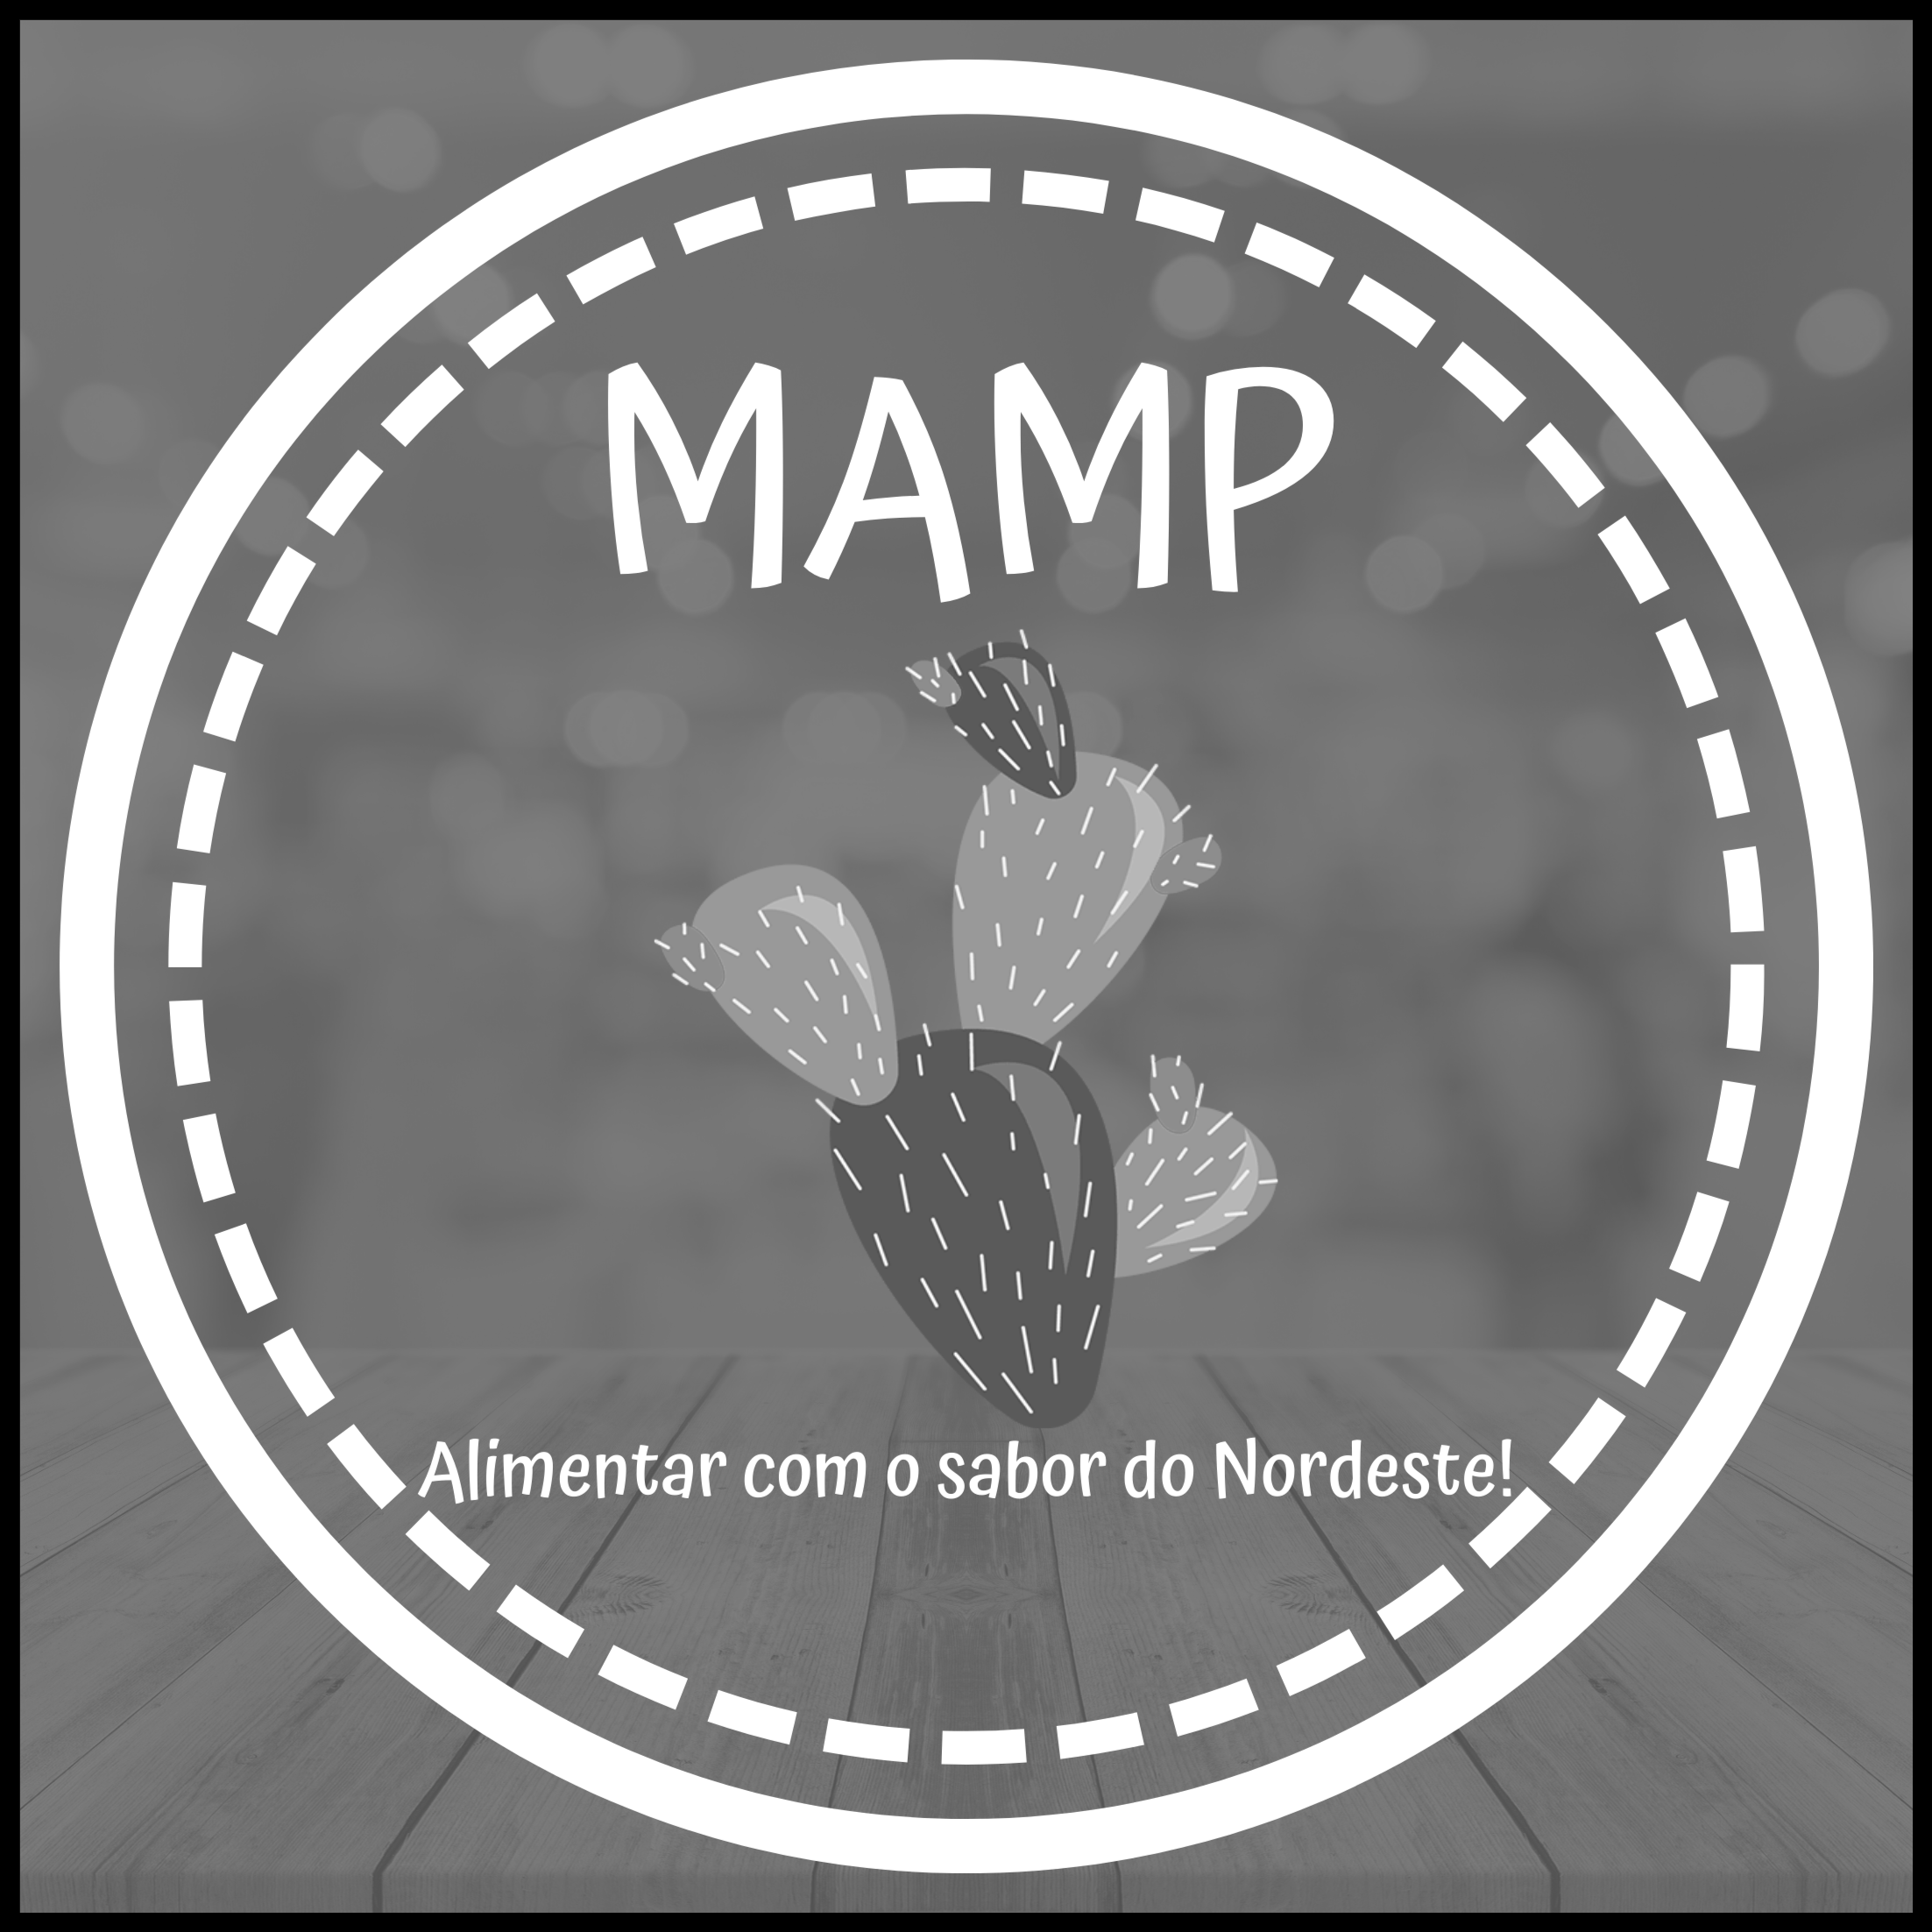
\includegraphics[scale=0.1]{Imagens/mamp.png}
\fonte{\cite{ufs_empreenda_2019}}
\label{figura_22}
\end{figure}



\subsection{Ranagro}

\textbf{PROBLEMA}

O mercado está cada vez mais competitivo, assim sendo necessário uma inovação para alcançar o resultado satisfatório e economicamente viável para o produtor e consumidor, além de trazer tecnologias inovadoras para o ramo da ranicultura. A qualidade e sustentabilidade é vista como uma arma de estratégia para a expansão da empresa. A carne de rã está sendo cada vez mais valorizada e consumida em restaurantes, no qual passou a ser recomendados por médicos e nutricionistas, pois sua taxa de gordura é de apenas três por cento, sendo a única carne produzida em cativeiros que possui dez aminoácidos e indicados também para alimentação de crianças que possuem rejeição à proteína animal, assim, podendo expandir cada vez mais seu consumo. A ração oferecida no mercado é mesma empregada na criação de peixes que acarreta um menor aproveitando da carne e elevando o custo para a engorda.

Assim a Ranagro, veio com uma proposta inovadora para o mercado que é a comercialização de uma ração específica, para haver um menor custo,menor impacto ambiental, crescimento rápido, boa lucratividade e um alto aproveitamento, no qual pode chegar muito próximo a cem por cento, se for considerado a exploração do mercado de subprodutos, como o fígado para pavê e a pele, que atende a medicina humana na recuperação de queimaduras. A ranicultura é uma nova oportunidade para ser explorada no agronegócio e a criação e comercialização da carne de rã, pode ser uma nova forma de ampliar o nicho agrário do país. Nosso grupo é formado por três graduastes de zootecnia e dois de engenharia agronômica, obrigada pela atenção de todos (Figura \ref{figura_26}).



\begin{figure}[H]
\centering
\caption{\textbf{Marca Ranagro}}

\includegraphics[scale=0.7]{Imagens/ranagro.png}
\fonte{\cite{ufs_empreenda_2019}}
\label{figura_26}
\end{figure}



\subsection{Tecno Coco}

A ideia da Tecno Coco é gerar uma cadeia cíclica de produção onde o Campo produz o coco, que é destinado ao comerciante, vendido ao usuário onde é descartado e processada pela nossa Startup retornando ao Campo como insumo agrícola, auxiliando na produtividade. Outra parte será destinada a outras cadeias produtivas e manufaturas, como material para isolamento acústico, reforço de materiais, enchimento de estofados, mantas para proteção do solo e muitos outros produtos que esse resíduo pode ser transformado.

Uma startup que está em fase de desenvolvimento por alunos da Universidade Federal de Sergipe e que tem como objetivo resolver o problema ambiental gerado pelo o acumulo de resíduos do coco no nosso estado (Figura \ref{figura_27}).

\begin{figure}[H]
\centering
\caption{\textbf{Marca Tecno Coco}}
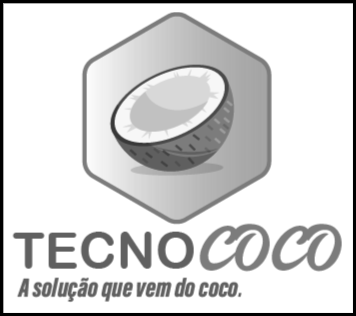
\includegraphics[scale=2.0]{Imagens/tecnococo.png}
\fonte{\cite{ufs_empreenda_2019}}
\label{figura_27}
\end{figure}



\subsection{Une Agro}

Imagine se uma fabrica produzisse uma produto que o único escoamento dele fosse para uma distribuidora na região, essa distribuidora ia ditar preço e quantidade que iria comprar os produtos, podendo até perder a produção. Qual incentivo essa fabrica teria de produzir? Bem isso acontece com diversos agricultores no Brasil, ficam refém apenas de um atravessador que vai até a porta dele para escoar seus produtos, sendo que o atravessador fica com maior parte dos lucros, e muitas vezes o que paga a agricultor é só o custo da produção.

A UneAgro pensando nisso, elaboramos um aplicativo onde o produtor possa anunciar seus produtos de forma pratica e rápida, sem sair de casa, onde ele irá ter uma amplo leque de clientes que estão interessados no produto dele.

O aplicativo é desenvolvido para as duas personas, tanto para agricultor quanto para o distribuidor, pois o distribuidor também sai ganhando ao utilizar o aplicativo pois terá uma maior quantidade localidade e preços pelo mesmo produto, podendo negociar com todas. O aplicativo será totalmente gratuito, sendo que a receita da empresa se originará nas parcerias anunciantes e seus produtos no aplicativo, além de disponibilizar informações produtos que serão disponibilizados para os usuários através de um pacote mensal ou anual, onde esses info-produtos estarão relacionados ao próprio desenvolvimento de negócio dos usuários, como aulas e \textit{podcasts} sobre gestão e produção agrícola (Figura \ref{figura_28}).

\begin{figure}[H]
\centering
\caption{\textbf{Marca Une Agro}}

\includegraphics[scale=1.5]{Imagens/uneagro.png}
\fonte{\cite{ufs_empreenda_2019}}
\label{figura_28}
\end{figure}



%\chapter{RESULTADOS E DISCUSSÃO }

\section{Alcance da amostra}



Para o desenvolvimento do programa foi alcançado 26 equipes apresentando ao todo 118 alunos oriundos dos cursos do centro de agrárias e mais outras áreas: \textit{Artes Visuais}, \textit{Administração}, \textit{Design Gráfico}, \textit{Engenharia Química}, \textit{Engenharia de Produção}, \textit{Marketing e Ecologia}. 



Os dados coletados revelam que, nas 63 respostas válidas que compõem a amostra, a divisão de gênero está equilibrada, sendo que 33 eram homens e 30 mulheres. Em relação à faixa etária quando realizaram o programa de mobilidade acadêmica, 67\% dos estudantes possuíam entre 19 e 22 anos e 30\% apresentaram a intervalo de idades entre 23 e 26 anos.



\begin{table}[!htb]
\caption{\textbf{Faixa etária dos alunos inscritos no programa}}
\label{tab:tabela_4}
\begin{tabular}{clccc}
\hline \hline
{\color[HTML]{000000} \textbf{Dados}} & {\color[HTML]{000000} \textbf{Faixa etária}} & \multicolumn{3}{c}{{\color[HTML]{000000} \textbf{Inscritos}}} \\ \cline{1-5}
{\color[HTML]{000000} } & {\color[HTML]{000000} } & \multicolumn{1}{l}{{\color[HTML]{000000} \textbf{Frequência (\%)}}} & \multicolumn{1}{l}{{\color[HTML]{000000} \textbf{Porcentagem (\%)}}} & \multicolumn{1}{l}{{\color[HTML]{000000} \textbf{Porcentagem válida (\%)}}} \\
{\color[HTML]{000000} } & {\color[HTML]{000000} \textbf{Menor que 20}} & {\color[HTML]{000000} 89} & {\color[HTML]{000000} 75,4} & {\color[HTML]{000000} 77,4}\\[8pt]
\multirow{-3}{*}{{\color[HTML]{000000} \textbf{}}} & {\color[HTML]{000000} \textbf{De 21 a 25}} & {\color[HTML]{000000} 19} & {\color[HTML]{000000} 16,1} & {\color[HTML]{000000} 16,5} \\[8pt]
\multicolumn{1}{l}{{\color[HTML]{000000} \textbf{Válidos}}} & {\color[HTML]{000000} \textbf{Maior que 25}} & {\color[HTML]{000000} 7} & {\color[HTML]{000000} 5,9} & {\color[HTML]{000000} 6,1}\\[8pt]
\multicolumn{1}{l}{{\color[HTML]{000000} \textbf{}}} & {\color[HTML]{000000} \textbf{Total}} & {\color[HTML]{000000} 115} & {\color[HTML]{000000} 97,5} & {\color[HTML]{000000} } \\[8pt]\hline
\multicolumn{1}{l}{{\color[HTML]{000000} \textbf{Omissos}}} & {\color[HTML]{000000} \textbf{Não informou}} & {\color[HTML]{000000} 3} & {\color[HTML]{000000} 2,5} & {\color[HTML]{000000} } \\[8pt] \hline
\multicolumn{2}{c}{{\color[HTML]{000000} \textbf{TOTAL GERAL}}} & {\color[HTML]{000000} 118} & {\color[HTML]{000000} } & {\color[HTML]{000000} } \\ \hline\hline
\end{tabular}
\fonte{Autoria própria}
\end{table}

O curso que mais apresentou inscrições dos alunos foi o de Engenharia Agronômica, representando 47,32\% deste total, enquanto os cursos de Engenharia Agrícola, Zootecnia, Engenharia de Pesca e Engenharia Florestal tiveram participações consideravelmente menores, com apenas 11,61\%, 19,64\%, 4,46\% e 6,25\% dos estudantes inscritos, respectivamente, já o curso de Medicina veterinária não apresentou alunos inscritos. Na figura  \ref{figura_10} é possível observar a quantidade de alunos inscritos e seus respectivos cursos.

\begin{figure}[!htb]
\centering
\caption{\textbf{Porcentagem de alunos inscritos no programa por curso}}
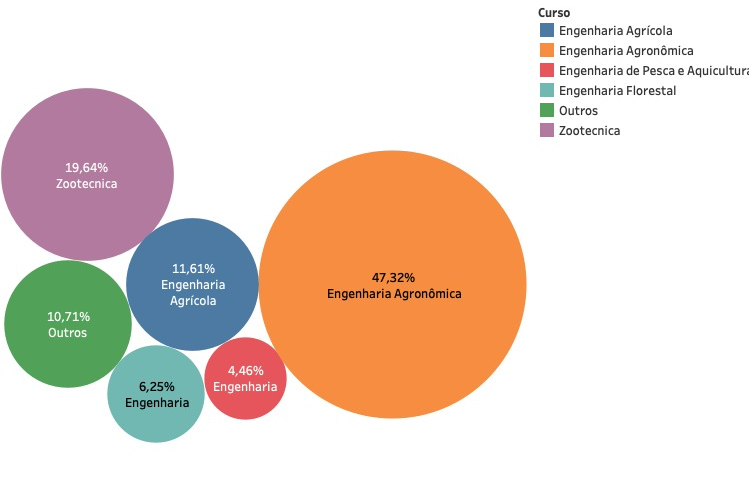
\includegraphics[scale=0.4]{Imagens/inscritos.png}
\fonte{Autoria própria}
\label{figura_10}
\end{figure}

\newpage

\section{Tratamento dos grupos de itens: Autoeficácia, Intenção empreendedora, Apoio Familiar}

O método de rotação Varimax com normalização de Kaiser\footnotemark[1] apresentou 3 componentes principais para esta pesquisa, aglutinando as questões na ordem apresentada na tabela \ref{tabela_3}:


\begin{center}
 %\large

\begin{longtable}{p{6cm} c c c }

\caption{\textbf{Estrutura fatorial da medida de intenção empreendedora}}

\label{tabela_3} \\ \hline\hline

\multicolumn{1}{p{6cm}}{} & \multicolumn{3}{c}{\textbf{Fatores}}\\ 
 \multicolumn{1}{c}{\textbf{Itens}} & \multicolumn{3}{c}{\hrulefill}\\ 

 \multicolumn{1}{c}{} 
 &\multicolumn{1}{p{1.5cm}}{\textbf{Autoeficácia}} & \multicolumn{1}{p{1.5cm}}{\textbf{Intenção}} &\multicolumn{1}{p{1.5cm}}{\textbf{Família}}  
\\ \hline 

\endfirsthead


\multicolumn{4}{l}{{{\bfseries \tablename \ \thetable{} -\ \textbf{Estrutura fatorial da medida de intenção empreendedora}}}}\\
\multicolumn{4}{r}{\bfseries \textbf{(continuação)}}\\

\hline \multicolumn{1}{p{6cm}}{\textbf{Questões}} &\multicolumn{1}{c}{\textbf{Autoeficácia}} & \multicolumn{1}{c}{\textbf{Intenção}} &\multicolumn{1}{c}{\textbf{Família}}  
\\ \hline 

\endhead

\hline \multicolumn{4}{r}{\textbf{(Continua)}} \\ \hline


\endfoot
\hline \multicolumn{4}{r}{\textbf{(Conclusão)}} \\ \hline
\hline \hline

\endlastfoot


Estabelecer e atingir metas e objetivos
 &  0,776 & & \\\\
 
Gerar novas ideias
 &  0,785 & & \\\\
 
Desenvolver novos produtos
 &  0,682 & & \\\\
 
Fazer análises financeiras
 &  0,739 & & \\\\
 
Reduzir riscos e incertezas
 &  0,746 & & \\\\
 
Assumir riscos calculados
 &   0,756 & & \\\\
 
 Tomar decisões em situações de risco
 &   0,637 & & \\\\
 
Administrar o tempo estabelecendo metas
 &   0,650 & & \\\\
 
Responsabilizar-me por ideias e decisões
 & 0,465
& \textbf{0,577} &  \\\\

Começar minha própria empresa
 & 0,456 & \textbf{0,592}  & \\\\
 
Para mim, ser um empreendedor implica em mais vantagens do que desvantagens
 &  & 0,894  & \\\\
 
Uma carreira como empreendedor é atrativa
 &  & 0,817  & \\\\
 
Se tivesse a oportunidade e os recursos, eu me tornaria um empreendedor
 &  & 0,892 & \\\\
 
Ser um empreendedor traria grande satisfação
 &  & 0,905 & \\\\
 
O capital oferecido por minha família e empréstimo em condições flexíveis são facilitadas
 &  & & 0,905 \\\\
 
Minha família me fornece contatos com pessoas que podem me ajudar na carreira de empreendedor
 &  & & 0,779 \\\\
 
Minha família me apresenta pessoas de sua rede de relação de negócios
 &  & & 0,621 \\\\
 
Minha família me transmite conhecimentos ligados ao meu setor de atividade
 &  & & 0,806 \\\\
 
Meus pais / minha família são meus mentores ou \textit{coachs} nas minhas atividades de empreendedor
 &  & & 0,820 \\\\
 
Minha família me fornece locais/ infraestrutura para minhas atividades de empreendedor.
 &  & & 0,682 \\\\
 
Meus pais ou família me concedem acesso a uma rede de distribuição para minha empresa.
 &  & & 0,722 \\\\
 
 Pensando em todos os possíveis recursos que minha família me fornece, sou completamente independente dela para decidir como alocá-los e usá-los.
 &  & & 0,661 \\\\
 
Minha família me empresta capital que  tenho que pagar regularmente a eles com juros		
 &  & & 0,692 \\\\
 
Minha família me empresta capital sem a necessidade de juros e que pode ser perdido se o negócio falir
 & & & 0,512 \\\\ \hline 
 
\end{longtable}
\fonte{Autoria própria}
\end{center}
\footnotetext[1]{Método de Extração: Análise de Componente Principal.\\Método de Rotação: Varimax com Normalização de Kaiser.}



\begin{table}[!htb]
 \label{tabela_4}
 \centering
\caption{\textbf{Variância total explicada}}
 \\ \hline\hline
\begin{tabular}{c c c c }
\multicolumn{1}{p{6cm}}{} & \multicolumn{3}{c}{\textbf{Fatores}}\\ 
 \multicolumn{1}{c}{\textbf{Itens}} & \multicolumn{3}{c}{\hrulefill}\\ 

 \multicolumn{1}{c}{} 
 &\multicolumn{1}{c}{\textbf{Autoeficácia}} & \multicolumn{1}{c}{\textbf{Intenção}} &\multicolumn{1}{c}{\textbf{Família}}  
\\\\ \hline 

 Somas de rotação de carregamentos ao quadrado (n)
 & 5,526 & 5,014 & 4,604 \\\\
 Variância explicada (\%)
 & 19,05 & 17,30 &15,87\\\\
 Variância cumulativa (\%)
 & 19,05\% & 36,34\% &52\% \\\hline \hline 
 
\end{tabular}
\fonte{Adaptado de \cite{lima_sauglobal_2017}}.
\end{table}



As questões: \textbf{"Para mim sem empresa não e autônomo"}, \textbf{"Eu já sou meu próprio patrão na empresa que eu fundei"} e \textbf{"Tenho precisão consistente do que empreender e datas para os passos da fundação"}, foram eliminadas da pesquisa, pois foi adotado a supressão de coeficientes que apresentaram valores absolutos a baixo de 0,40, Já as questões: \textbf{Responsabilizar-me por ideias e decisões} e \textbf{Começar minha própria empresa}, apresentaram valores satisfatórios tanto para dimensão Autoeficácia quanto para dimensão intenção empreendedora, porem foi considerado o valor de coeficiente mais alto.


\section{Resultados do estudo}

Os resultados encontram-se divididos em seções, atendendo aos objetivos do estudo. Inicialmente  serão  apresentadas  descrições  que  caracterizam  os  dois  grupos  (pré-programa  e pós-programa) em relação às variáveis e as comparações entre os grupos.

\subsection{Áreas e cadeias produtivas}


A fase inicial do programa foram alcançadas 27 propostas de protótipos e/ou negócios na área rural com foco na agricultura sustentável. Na figura \ref{figura_11} é possível verificar as áreas e cadeias produtivas prioritárias escolhidas.


\begin{figure}[!H]
\centering
\caption{\textbf{Áreas e potenciais propostas de negócios escritos}}
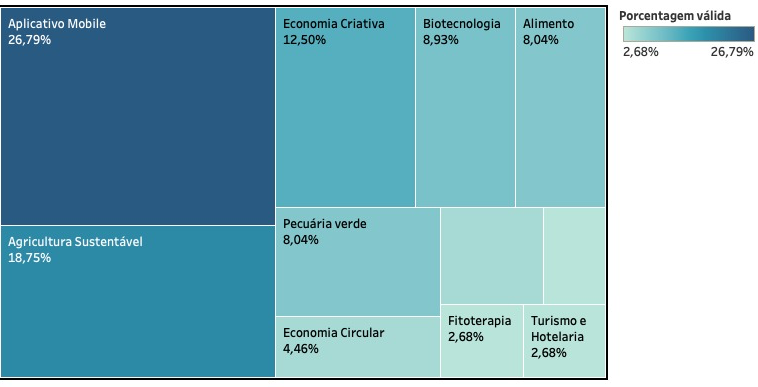
\includegraphics[scale=0.5]{Imagens/propostas_negocios.png}
\fonte{Autoria própria}
\label{figura_11}
\end{figure}


\chapter{CONSIDERAÇÕES FINAIS}


Com o desenvolvimento deste estudo, pode-se perceber que, os objetivos propostos pelo Programa Empreenda Agro Sustentável foram contemplados na medida em que foram mobilizados vários estudantes de graduação as ciências agrarias e de outras áreas do conhecimento da UFS, em um desafio de criarem propostas de startups se utilizando de metodologias ativas, numa fase de pré-aceleração. Nesse sentido, 15 equipes apresentaram seus Modelos de Negócio com bastante consistência, atraindo a atenção de investidores, ou se colocando para discussão com aceleradoras, que se dispuserem na busca de investidores. Desta feita, as universidades e faculdades sempre podem fazer mais para fornecer assistência de qualidade no fomento da autoeficácia e intenção empreendedora dos alunos e de uma boa escolha de carreira, em geral.

Os resultados iniciais mostram que cursos que promovem a educação empreendedora e a percepção favorável de um ambiente universitário empresarial influenciam positivamente duas das três principais competências estudadas, que influenciam o surgimento da educação empreendedora nos alunos dos cursos das ciências agrárias, que são: Autoeficácia, Intenção Empreendedora. Outro aspecto de grande relevância foi a atratividade do Programa de muitos parceiros que se dispuseram a apoiar a realização de todas as etapas da jornada de diversas formas.

A melhoria da Educação Empreendedora no ensino superior, especialmente aos cursos das ciências agrárias, com ênfase, na prática, e no contato com os novos empreendimentos, pode contribuir diretamente para a formação de profissionais, mais capazes de gerar novos negócios escaláveis, já que a intenção empreendedora em conjunto com a autoeficácia pode ser influenciada para melhora por programas educacionais, como já sustentou os resultados deste trabalho.

Embora o apoio educacional influencie positivamente as dimensões, a participação familiar se mostrou influenciável quando observados trabalhos de educação nas fases inicias dos negócios tal qual este programa estudado. Esses resultados aprofundam a pesquisa empírica existente sobre o assunto, uma vez que a família se apresenta como uma bolha eudaimônica, financiamento os empreendimentos e pivotagem, apoiando quando necessário os futuros empreendedores.

O desenvolvimento de ferramentas auxiliares tais como o aplicativo Empreenda Agro Sustentável, alcançou o propósito, que foi de, servir como uma ferramenta para aprimorar os conteúdos ministrados sobre empreendedorismo sustentável no meio rural, fornecendo acesso a informações e ajudando a motivar o envolvimento com o auto-gerenciamento dos alunos participantes do programa. Esses objetivos foram atendidos adequadamente, oferecendo aos usuários participantes a oportunidade de revisar, reforçar e dispor de conteúdos direcionados.

O aplicativo também pode ser indicado para profissionais que tenham interesse em aprender mais sobre o desenvolvimento de negócios sustentáveis e escaláveis. O aplicativo já possui registro no Instituto Nacional de Propriedade Industrial INPI sob número de registro \textbf{BR 51 2019 002657 8} e disponível gratuitamente para testes na loja online \textit{Google Play Store}.

Ao longo desta dissertação foram abordadas reflexões sobre as características da educação empreendedora através de um programa de extensão organizado por workshops encadeados. Educar é um processo complexo, que exige mudanças pessoais e institucionais significativas que levam tempo e investimento na formação de professores e desenvolvimento cultural nos alunos, para o domínio das intenções empreendedoras.

Neste sentido se recomenda em futuros trabalhos, explorar dinâmicas que abordem por mais tempo, os conteúdos aqui ministrados para que seja possível, analisar as mudanças comportamentais que surgem com as mudanças da intenção empreendedora, assim como inovações resultantes.

\hl{O programa esta dando continuidade com o Fórum Agro Sustentável assim como o I Simpósio Agro Sustentável}
%\chapter{Trabalhos Relacionados}

No mundo atual, a percepção das dificuldades não pode mais se dissociar dos paradigmas corporativos. Ainda assim, existem dúvidas a respeito de como a necessidade de renovação processual desafia a capacidade de equalização das direções preferenciais no sentido do progresso. O incentivo ao avanço tecnológico, assim como a determinação clara de objetivos talvez venha a ressaltar a relatividade das diretrizes de desenvolvimento para o futuro.

\section{Figuras}

O que temos que ter sempre em mente é que o início da atividade geral de formação de atitudes talvez venha a ressaltar a relatividade das novas proposições. Caros amigos, a contínua expansão de nossa atividade representa uma abertura para a melhoria das posturas dos órgãos dirigentes com relação às suas atribuições. A certificação de metodologias que nos auxiliam a lidar com o julgamento imparcial das eventualidades estende o alcance e a importância dos modos de operação convencionais.

\begin{figure}[htb]
	\caption{\label{fig_circulo}A delimitação do espaço}
	\begin{center}
	    \setlength{\unitlength}{5cm}
		\begin{picture}(1,1)
		\put(0,0){\line(0,1){1}}
		\put(0,0){\line(1,0){1}}
		\put(0,0){\line(1,1){1}}
		\put(0,0){\line(1,2){.5}}
		\put(0,0){\line(1,3){.3333}}
		\put(0,0){\line(1,4){.25}}
		\put(0,0){\line(1,5){.2}}
		\put(0,0){\line(1,6){.1667}}
		\put(0,0){\line(2,1){1}}
		\put(0,0){\line(2,3){.6667}}
		\put(0,0){\line(2,5){.4}}
		\put(0,0){\line(3,1){1}}
		\put(0,0){\line(3,2){1}}
		\put(0,0){\line(3,4){.75}}
		\put(0,0){\line(3,5){.6}}
		\put(0,0){\line(4,1){1}}
		\put(0,0){\line(4,3){1}}
		\put(0,0){\line(4,5){.8}}
		\put(0,0){\line(5,1){1}}
		\put(0,0){\line(5,2){1}}
		\put(0,0){\line(5,3){1}}
		\put(0,0){\line(5,4){1}}
		\put(0,0){\line(5,6){.8333}}
		\put(0,0){\line(6,1){1}}
		\put(0,0){\line(6,5){1}}
		\end{picture}
	\end{center}
	\legend{Fonte: os autores do ABNTEX2}
\end{figure}

\begin{figure}[!htb]
	\caption{Figura 1 - Imagens de STS sem atividade e com alta atividade respectivamente..
}
  \centering
  \includegraphics[scale=1.0]{Imagens/imagem_1.png} 
  
  \legend{Fonte: Gerador de Lero Lero}
  \label{figura0}
\end{figure}

Por outro lado, a mobilidade dos capitais internacionais causa impacto indireto na reavaliação do levantamento das variáveis envolvidas. Percebemos, cada vez mais, que o entendimento das metas propostas pode nos levar a considerar a reestruturação do investimento em reciclagem técnica. Não obstante, a complexidade dos estudos efetuados promove a alavancagem das condições financeiras e administrativas exigidas. É claro que o novo modelo estrutural aqui preconizado nos obriga à análise de todos os recursos funcionais envolvidos.

\section{Tabelas}

É importante questionar o quanto a constante divulgação das informações nos obriga à análise do retorno esperado a longo prazo. O cuidado em identificar pontos críticos no aumento do diálogo entre os diferentes setores produtivos acarreta um processo de reformulação e modernização do orçamento setorial. Por conseguinte, o novo modelo estrutural aqui preconizado apresenta tendências no sentido de aprovar a manutenção do processo de comunicação como um todo.

\begin{table}[htb]
\ABNTEXfontereduzida
\caption[Níveis de investigação]{Níveis de investigação.}
\label{tab-nivinv}
\begin{tabular}{p{2.6cm}|p{6.0cm}|p{2.25cm}|p{3.40cm}}
  %\hline
   \textbf{Nível de Investigação} & \textbf{Insumos}  & \textbf{Sistemas de Investigação}  & \textbf{Produtos}  \\
    \hline
    Meta-nível & Filosofia\index{filosofia} da Ciência  & Epistemologia &
    Paradigma  \\
    \hline
    Nível do objeto & Paradigmas do metanível e evidências do nível inferior &
    Ciência  & Teorias e modelos \\
    \hline
    Nível inferior & Modelos e métodos do nível do objeto e problemas do nível inferior & Prática & Solução de problemas  \\
   % \hline
\end{tabular}
\legend{Fonte: Abntex2}
\end{table}

Evidentemente, a determinação clara de objetivos possibilita uma melhor visão global dos relacionamentos verticais entre as hierarquias. Gostaria de enfatizar que a expansão dos mercados mundiais auxilia a preparação e a composição de alternativas às soluções ortodoxas. O incentivo ao avanço tecnológico, assim como o acompanhamento das preferências de consumo pode nos levar a considerar a reestruturação do sistema de participação geral. Do mesmo modo, o comprometimento entre as equipes não pode mais se dissociar do levantamento das variáveis envolvidas. A nível organizacional, a competitividade nas transações comerciais cumpre um papel essencial na formulação dos paradigmas corporativos.

\begin{table}[htb]
\IBGEtab{%
  \caption{Um Exemplo de tabela alinhada que pode ser longa
  ou curta, conforme padrão IBGE.}%
  \label{tabela-ibge}
}{%
  \begin{tabular}{cccc}
  \toprule
   Nome & Nascimento & Documento & Data \\
  \midrule \midrule
   Maria da Silva & 11/11/1111 & 111.111.111-11 \\
  \midrule 
   João Souza & 11/11/2111 & 211.111.111-11 \\
  \midrule 
   Laura Vicuña & 05/04/1891 & 3111.111.111-11 \\
  \bottomrule
\end{tabular}%
}{%
  \fonte{Produzido pelos autores.}%
  \nota{Esta é uma nota, que diz que os dados são baseados na
  regressão linear.}%
  \nota[Anotações]{Uma anotação adicional, que pode ser seguida de várias
  outras.}%
  }
\end{table}

\section{Considerações Finais}

Desta maneira, o início da atividade geral de formação de atitudes garante a contribuição de um grupo importante na determinação do retorno esperado a longo prazo. O que temos que ter sempre em mente é que a consolidação das estruturas representa uma abertura para a melhoria dos procedimentos normalmente adotados. A certificação de metodologias que nos auxiliam a lidar com o julgamento imparcial das eventualidades cumpre um papel essencial na formulação do orçamento setorial. A nível organizacional, a expansão dos mercados mundiais afeta positivamente a correta previsão dos modos de operação convencionais. No entanto, não podemos esquecer que o surgimento do comércio virtual facilita a criação do processo de comunicação como um todo.

Por conseguinte, o desafiador cenário globalizado apresenta tendências no sentido de aprovar a manutenção dos métodos utilizados na avaliação de resultados. Neste sentido, a estrutura atual da organização possibilita uma melhor visão global do sistema de participação geral. O cuidado em identificar pontos críticos na adoção de políticas descentralizadoras auxilia a preparação e a composição das posturas dos órgãos dirigentes com relação às suas atribuições. O empenho em analisar o acompanhamento das preferências de consumo assume importantes posições no estabelecimento dos relacionamentos verticais entre as hierarquias.
\bibliography{references}

% ----------------------------------------------------------
% ELEMENTOS PÓS-TEXTUAIS
% ----------------------------------------------------------

\postextual
\renewcommand{\chapnumfont}{\chaptitlefont}
\renewcommand{\afterchapternum}{}
\begin{apendicesenv}

% Imprime uma página indicando o início dos apêndices
\partapendices

% ----------------------------------------------------------
% ----------------------------------------------------------
% -------------------------------------------------------


\appendix


\chapter{Materiais disponibilizados no aplicativo}
\label{chap:tabela_2}
\begin{longtable}{p{3.5cm}p{11.0cm}}

\caption[\textbf{Materiais disponibilizados no aplicativo}]{\textbf{Conteúdos difundidos pelo aplicativo empreenda agro sustentável}} 
\label{tabela_2} \\

\hline \hline \multicolumn{1}{p{3.5cm}}{\textbf{Base de assuntos}} & \multicolumn{1}{c}{\textbf{Conteúdos}}\\ \hline 

\endfirsthead

\multicolumn{2}{c}%

{{ \bfseries \tablename \ \thetable{} - \ \textbf{Continuação}}}\\

    \hline \multicolumn{1}{p{3.5cm}}{\textbf{Métodos, Técnicas e Recursos}} & \multicolumn{1}{c}{\textbf{Aplicações}}  \\ \hline 

\endhead

\hline \multicolumn{2}{r}{{\textbf{Continua}}} \\ \hline

\endfoot
\hline \multicolumn{2}{r}{{\textbf{Continua}}} \\ \hline

\endfoot
\hline \multicolumn{2}{r}{{\textbf{Conclusão}}} \\ \hline
\hline \hline

\endlastfoot

Conceitos Básicos de Ideação & Insights; Startup Enxuta: Visão, direção e aceleração; Design thinking: Preparação, Ideação I, II e II, finalizando a descoberta \cite{alt_design_2018}. \\

Conceitos Básicos de modelo de negócio (CANVAS) & Briefing, seguimentos de clientes, proposta de valor, canais, relacionamento com clientes e fontes de Receitas, atividades-Chave e estrutura de Custo. \cite{finocchio_junior_project_2013} \\

Conceitos Básicos de Gestão ágil & Gerência do projeto ágil, manifesto Ágil: liderança e organização com Uscrum, início, planejamento e execução do projeto com Agile; Revisão, retrospectiva e encerramento de projetos com Agile, \cite{abrahamsson_agile_2017}. \\ 

Conceitos Básicos da Marketing & Marketing pessoal; Marketing digital/e-commerce: E-mail Marketing: Segmentação ao AB, introdução aos canais não pagos; Google Analytics; Shopify e Inteligência comercial. \cite{ritossa_marketing_2009, rizzo_marketing_2017}. \\ 

Conceitos Básicos da Marketing
Conceitos Básicos de Propriedade Intelectual
 & Direito autoral, Propriedade Industrial e Proteção Sui Generis, \cite{wipo_guide_2019} \\ 

\end{longtable}
\fonte{O autor}

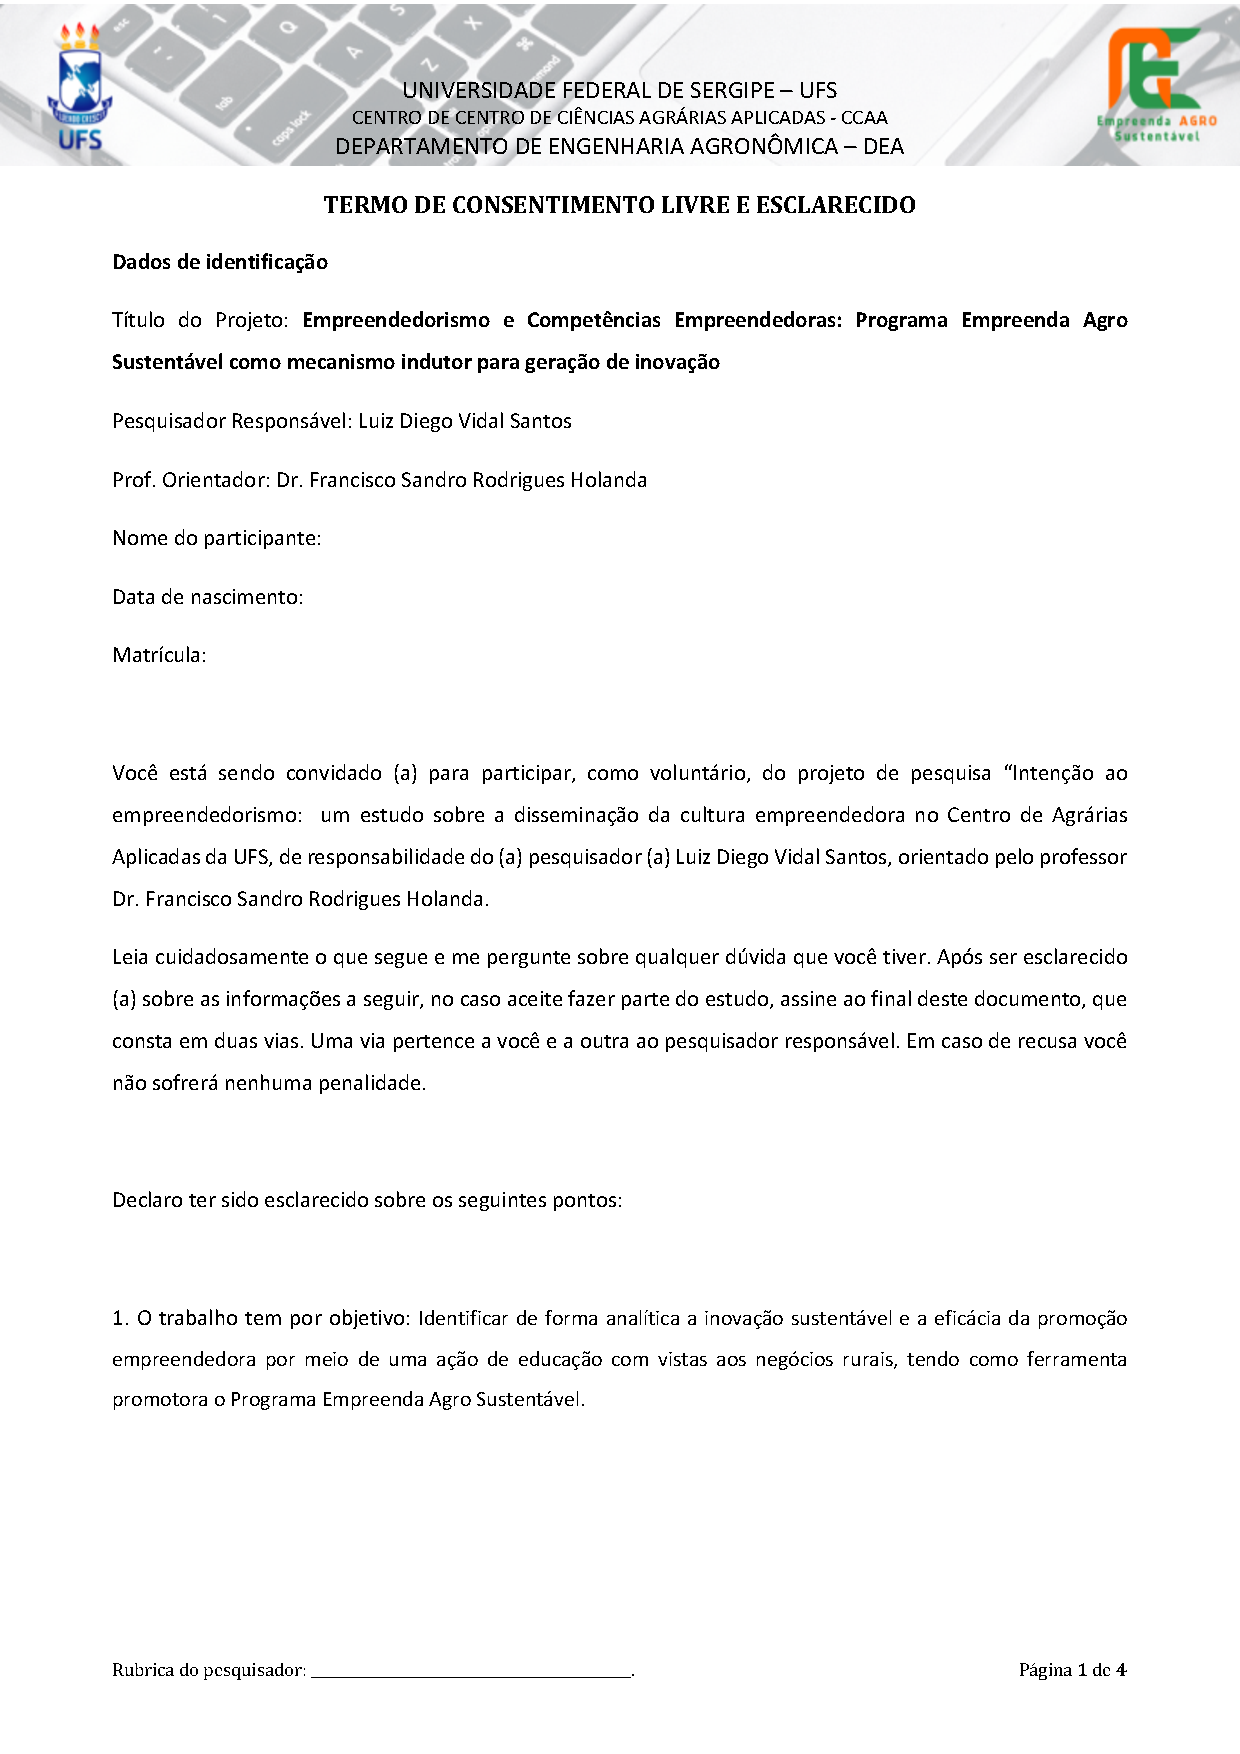
\includepdf[scale=0.80,pagecommand=\chapter{Termo de Consentimento Livre e Esclarecido TCLE}]{apendece/Termo.pdf}


%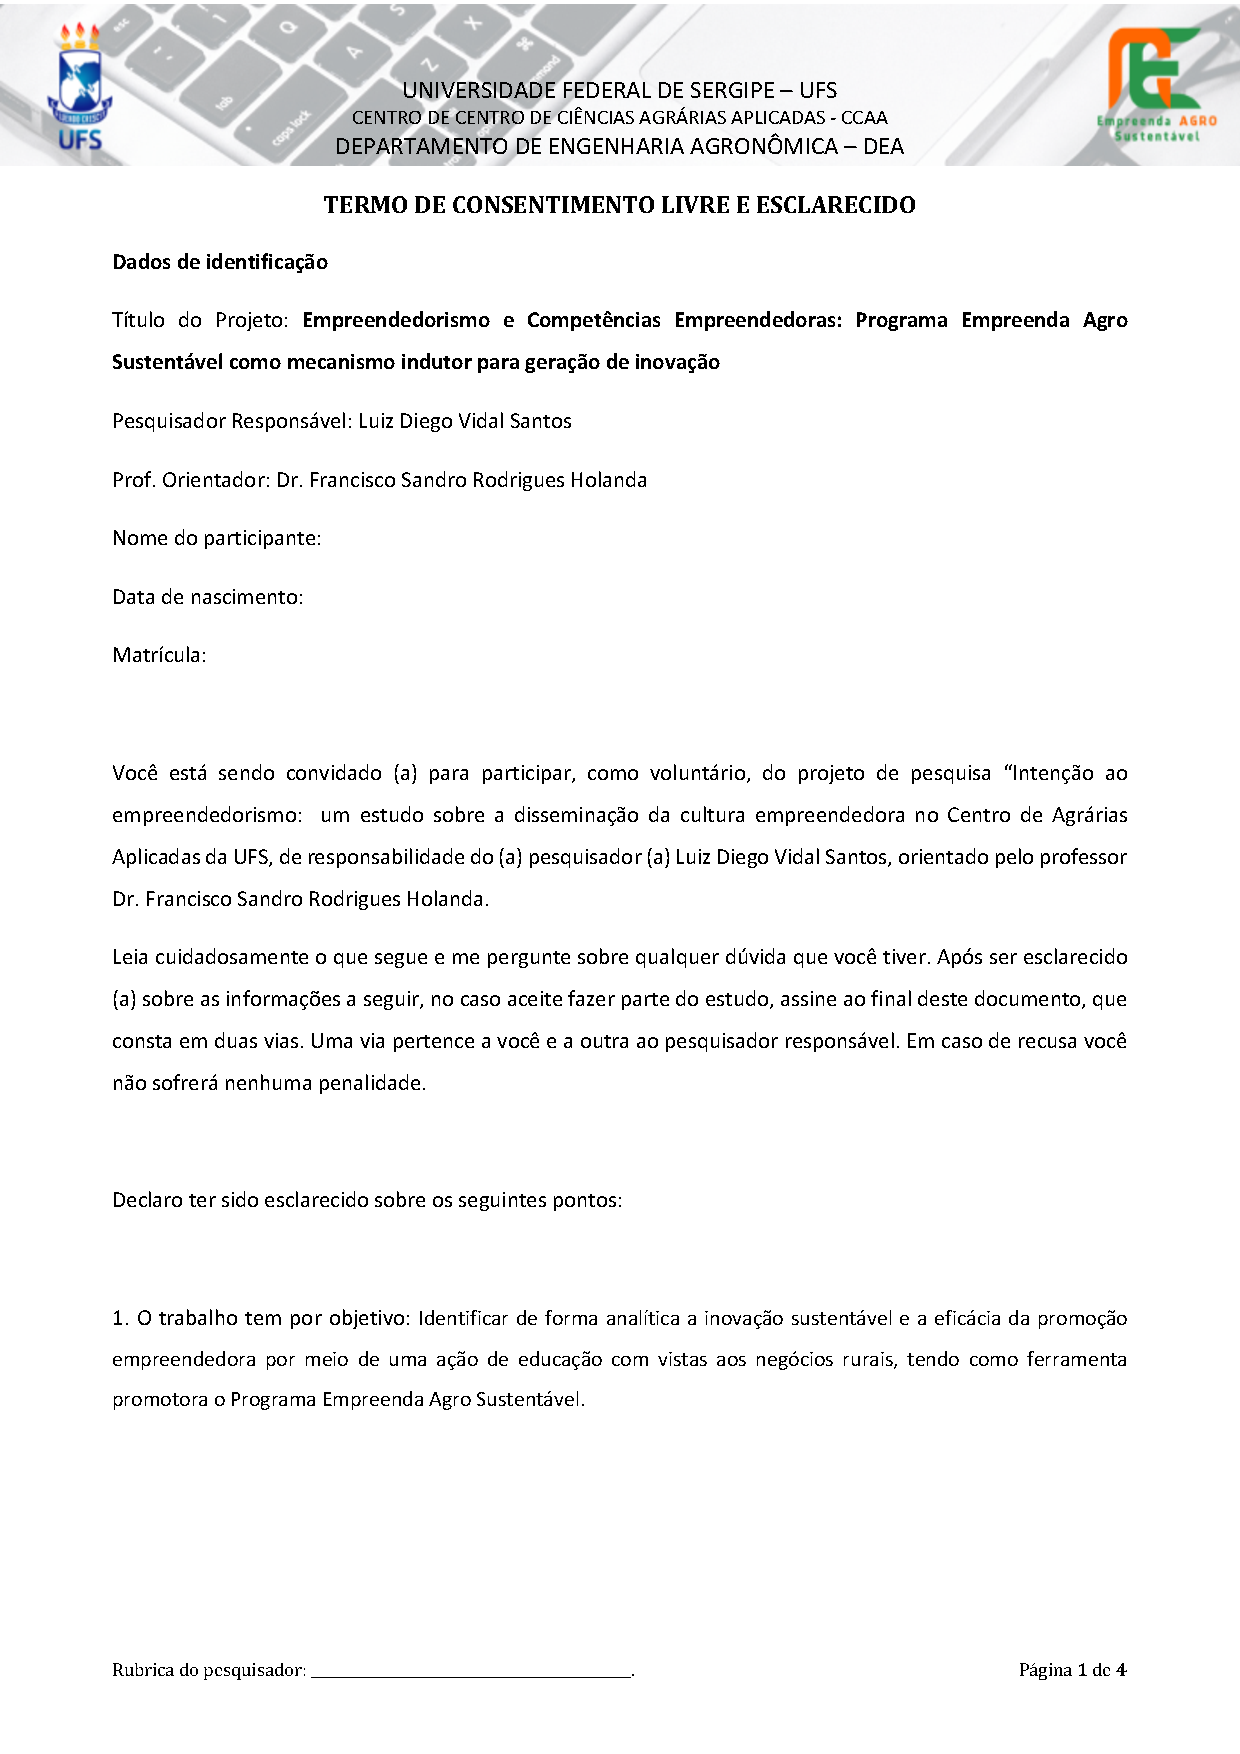
\includepdf[scale=0.87, pagecommand=\chapter{Termo de Consentimento Livre e Esclarecido TCLE}]{apendece/Termo.pdf}


\chapter{Estrutura fatorial da medida de intenção empreendedora}
\label{chap:tabela_3}

\begin{longtable}[H]{p{6cm} c c c }
\caption{\textbf{Estrutura fatorial da medida de intenção empreendedora}}
\label{tabela_3}\\
\hline \hline
\multicolumn{1}{p{6cm}}{} & \multicolumn{3}{c}{\textbf{Fatores}}\\ 
 \multicolumn{1}{c}{\textbf{Itens}} & \multicolumn{3}{c}{\hrulefill}\\ 

 \multicolumn{1}{c}{} 
 &\multicolumn{1}{p{1.5cm}}{\textbf{Autoeficácia}} & \multicolumn{1}{p{1.5cm}}{\textbf{Intenção}} &\multicolumn{1}{p{1.5cm}}{\textbf{Família}}  
\\ \hline 

\endfirsthead

\multicolumn{4}{l}{{{\bfseries \tablename \ \thetable{} -\ \textbf{Estrutura fatorial da medida de intenção empreendedora}}}}\\
\multicolumn{4}{r}{\bfseries \textbf{(continuação)}}\\

\hline \multicolumn{1}{p{6cm}}{\textbf{Questões}} &\multicolumn{1}{c}{\textbf{Autoeficácia}} & \multicolumn{1}{c}{\textbf{Intenção}} &\multicolumn{1}{c}{\textbf{Família}}  
\\ \hline 

\endhead

\hline \multicolumn{4}{r}{\textbf{(Continua)}} \\ \hline


\endfoot
\hline \multicolumn{4}{r}{\textbf{(Conclusão)}} \\ \hline
\hline \hline

\endlastfoot


Estabelecer e atingir metas e objetivos
 &  ,752 & & \\\\
 
Gerar novas ideias
 &  ,702 & & \\\\
 
Desenvolver novos produtos
 &  ,772 & & \\\\
 
Fazer análises financeiras
 &  ,547 & & \\\\
 
Reduzir riscos e incertezas
 &  ,683 &  & \\\\
 
Assumir riscos calculados
 &   ,463 & \textbf{,451} & \\\\
 
Tomar decisões em situações de risco
 &   ,522 & & \\\\
 
Administrar o tempo estabelecendo metas
 &   ,649 & & \\\\
 
Responsabilizar-me por ideias e decisões
 & ,456 & &  \\\\
 
Começar minha própria empresa
& ,603 & \textbf{,435}  & \\\\

Conduzir minha própria empresa ao sucesso
 & ,658 & \textbf{,470}  & \\\\
Eu já sou meu próprio patrão na empresa que eu fundei
 & & ,430 &  \\\\

Para mim, ser um empreendedor implica em mais vantagens do que desvantagens
 &  & ,727  & \\\\
 
Uma carreira como empreendedor é atrativa
 &  & ,890  & \\\\
 
Se tivesse a oportunidade e os recursos, eu me tornaria um empreendedor
 &  & ,788 & \\\\
 
Ser um empreendedor traria grande satisfação
 &  & ,821 & \\\\
 
Por gentileza, indique quão seriamente tem pensado em criar seu próprio negócio
 &  & ,588 & \\\\
 
O capital oferecido por minha família e empréstimo em condições flexíveis são facilitadas
 &  & & ,618 \\\\
 
Minha família me fornece contatos com pessoas que podem me ajudar na carreira de empreendedor
 &  & & ,658 \\\\
 
Minha família me apresenta pessoas de sua rede de relação de negócios
 &  & & ,400 \\\\
 
Minha família me transmite conhecimentos ligados ao meu setor de atividade
 &  & & ,618 \\\\
 
Meus pais / minha família são meus mentores ou \textit{coachs} nas minhas atividades de empreendedor
 &  & & ,687 \\\\
 
Minha família me fornece locais/ infraestrutura para minhas atividades de empreendedor.
 &  & & ,658 \\\\
 
Meus pais ou família me concedem acesso a uma rede de distribuição para minha empresa.
 &  & & ,702 \\\\
 
 
Minha família me empresta capital que  tenho que pagar regularmente a eles com juros		
 &  & & ,583 \\\\
 
Minha família me empresta capital sem a necessidade de juros e que pode ser perdido se o negócio falir
 & & & ,556 \\\\ \hline 
 
\end{longtable}
\fonte{O Autor}
\footnotetext[1]{Método de Extração: Análise de Componente Principal.\\Método de Rotação: Varimax com Normalização de Kaiser.}

\chapter{Teste de amostras independentes para as questões relacionadas a autoeficácia}
\label{tab:amostras_autoeficacia}


\begin{longtable}[H]{p{7cm}ccccc}
\caption{\textbf{Teste de amostras independentes para as questões relacionadas a autoeficácia}}
\label{tabela_5}\\
\hline \hline
 &
  \multicolumn{1}{l}{} &
  \multicolumn{1}{l}{} &
  \multicolumn{1}{l}{} &
  \multicolumn{1}{l}{} &
  \multicolumn{1}{l}{} \\
\endfirsthead
%
\multicolumn{6}{c}
{{Tabela \thetable\ - Teste de amostras independentes}} \\
\multicolumn{6}{r}{\textbf{(Continuação)}}
\\ \hline
%
\endhead
%
\endfoot
\hline \multicolumn{6}{r}{\textbf{(Conclusão)}} \\
\hline \hline

\endlastfoot
%
\multicolumn{1}{c}{\textbf{Teste de amostras independentes}} &
  \multicolumn{2}{c}{\textbf{Mediana}} &
  \multicolumn{2}{c}{\textbf{Posto Médio}} &
  \multicolumn{1}{c}{\textbf{\textit{P-value}}} \\ \cline{2-6}
 &
  \textbf{antes} &
  \multicolumn{1}{l}{\textbf{após}} &
  \textbf{antes} &
  \textbf{após} &
  \multicolumn{1}{l}{} \\ \hline
Estabelecer e atingir metas e objetivos &
  5 &
  6 &
  65,36 &
  75,94 &
  0,114 \\
Gerar novas ideias &
  6 &
  6 &
  65,27 &
  76,07 &
  0,110 \\
Desenvolver novos produtos & %Falta fazer
  4 &
  6 &
  61,13 &
  76,06 &
  0,950 \\
Fazer análises financeiras &
  4 &
  6 &
  61,13 &
  76,06 &
  \textbf{0,002} \\
Reduzir riscos e incertezas &
  3 &
  5 &
  58,69 &
  86,31 &
  \textbf{0,000} \\
Assumir riscos calculados &
  4 &
  5 &
  63,08 &
  79,49 &
  \textbf{0,016} \\
Tomar decisões em situações de risco &
  5 &
  5 &
  69,55 &
  69,43 &
  0,986 \\
Administrar o tempo estabelecendo metas &
  5 &
  6 &
  63,50 &
  78,83 &
  \textbf{0,023} \\
Responsabilizar-me por ideias e decisões &
  5 &
  6 &
  64,41 &
  77,42 &
  0,053 \\\hline \hline
\end{longtable}
\fonte{O Autor}

\chapter{Testes de amostras independentes para Participação Familiar e influência de terceiros}
\label{tab:amostras_familiar}

\begin{longtable}[!h]{p{7cm}ccccc}
\caption{\textbf{Testes de amostras dependentes para Participação familiar e influência de terceiros}}
\label{tabela_familair}\\
\hline \hline
 &
  \multicolumn{1}{l}{} &
  \multicolumn{1}{l}{} &
  \multicolumn{1}{l}{} &
  \multicolumn{1}{l}{} &
  \multicolumn{1}{l}{} \\
\endfirsthead
%
\multicolumn{6}{c}
{{Tabela \thetable\ - Testes de amostras independentes para Participação familiar e influência de terceiros}} \\
\multicolumn{6}{r}{\textbf{(Continuação)}}
\\ \hline
%
\endhead
%
\endfoot
\hline \multicolumn{6}{r}{\textbf{(Conclusão)}} \\
\hline \hline

\endlastfoot
%
\multicolumn{1}{c}{\textbf{Teste de amostras independentes}} &
  \multicolumn{2}{c}{\textbf{Mediana}} &
  \multicolumn{2}{c}{\textbf{P. Médio}} &
  \multicolumn{1}{c}{\textbf{\textit{P-value}}} \\ \cline{2-5}
 &
  \textbf{antes} &
  \multicolumn{1}{l}{\textbf{após}} &
  \textbf{antes} &
  \textbf{após} &
  \multicolumn{1}{l}{} \\ \hline
O capital oferecido por minha família é um empréstimo em condições flexíveis e facilitadas (p. ex.: baixas taxas de juros) &
  2 &
  1 &
  73,12 &
  62,67 &
    0,104 \\
Minha família me apresenta pessoas de sua rede de relação de negócios, oferecendo me contato com possíveis parceiros e/ou clientes &
  3 &
  1 &
  74,66 &
  60,31 &
 \textbf{0,030} \\
Minha família me transmite conhecimentos ligados ao meu setor de atividade sobre como oferecer serviços e como produzir os produtos &
  2 &
  1 &
  72,93 &
  60,61 &
  0,056 \\
Meus pais / minha família são meus mentores ou coachs nas minhas atividades de empreendedor &
  2 &
  1 &
  69,41 &
  65,88 &
  0,079 \\
Minha família me fornece locais/ infraestrutura para minhas atividades de empreendedor &
  2 &
  1 &
  71,96 &
  63,25 &
  0,179 \\
Meus pais/minha família me concedem acesso a uma rede de distribuição para minha empresa &
  1 &
  1 &
  60,30 &
  72,51 &
  \textbf{0,045} \\
Pensando em todos os possíveis recursos que minha família me fornece, eu sou completamente dependente dela para decidir como alocá-los e usá-los &
  3 &
  3 &
  69,99 &
  65,02 &
  0,455 \\
O capital oferecido por minha família é um empréstimo em condições flexíveis e facilitadas &
  1 &
  1 &
  75,01 &
  58,61 &
  0,0808 \\
Minha família me empresta capital que eu tenho que pagar regularmente a eles com juros &
  1 &
  1 &
  69,63 &
  68,03 &
  0,783 \\
Minha família me empresta capital sem a necessidade de sem juros e que pode ser perdido se o negócio falir &
  2 &
  1 &
  72,11 &
  64,21 &
  0,205  \\ \hline \hline
\end{longtable}
\fonte{O Autor}


\chapter{Teste de amostras independentes para Intenção Empreendedora}
\label{tab:amostras_intencao_empreendedora}


\begin{longtable}[!h]{p{7cm}ccccc}
\caption{\textbf{Teste de amostras independentes para Intenção Empreendedora}}
\label{tabela_6}\\
\hline \hline
 &
  \multicolumn{1}{l}{} &
  \multicolumn{1}{l}{} &
  \multicolumn{1}{l}{} &
  \multicolumn{1}{l}{} &
  \multicolumn{1}{l}{} \\
\endfirsthead
%
\multicolumn{6}{c}
{{Tabela \thetable\ - Teste de amostras independentes  para Intenção Empreendedora}} \\
\multicolumn{6}{r}{\textbf{(Continuação)}}
\\ \hline
%
\endhead
%
\endfoot
\hline \multicolumn{6}{r}{\textbf{(Conclusão)}} \\
\hline \hline

\endlastfoot
%
\multicolumn{1}{c}{\textbf{Teste de amostras independentes}} &
  \multicolumn{2}{c}{\textbf{Mediana}} &
  \multicolumn{2}{c}{\textbf{P. Médio}} &
  \multicolumn{1}{c}{\textbf{\textit{P-value}}} \\ \cline{2-5}
 &
  \textbf{antes} &
  \multicolumn{1}{l}{\textbf{após}} &
  \textbf{antes} &
  \textbf{após} &
  \multicolumn{1}{l}{} \\ \hline
Começar minha própria empresa &
  5 &
  6 &
  65,66 &
  75,47 &
    0,151 \\
Conduzir minha própria empresa ao sucesso &
  5 &
  6 &
  65,46 &
  74,51 &
  0,177 \\
Eu já sou meu próprio patrão na empresa que eu fundei &
  1 &
  1 &
  72,76 &
  61,83 &
  0,077 \\
Para mim, ser um empreendedor implica em mais vantagens do que desvantagens &
  6 &
  6 &
  65,00 &
  75,34 &
  0,122 \\
Uma carreira de empreendedor é atrativa para mim &
  6 &
  6,5 &
  65,24 &
  73,60 &
  0,202 \\
Se tivesse oportunidade e os recursos eu me tornaria um empreendedor &
  7 &
  7 &
  60,30 &
  72,51 &
  \textbf{0,045} \\
Ser empreendedor me traria grande satisfação &
  6 &
  7 &
  64,39 &
  76,31 &
  0,069 \\
Por gentileza, indique quão seriamente tem pensado em criar seu próprio negócio &
  6 &
  6 &
  64,96 &
  75,41 &
  0,119 \\
Eu já sou patrão na empresa que criei &
  6 &
  6 &
  72,76 &
  61,83 &
  0,077 \\
Tenho pensado em abrir minha empresa &
  6 &
  6 &
  66,67 &
  72,70 &
  0,377  \\ \hline \hline
\end{longtable}
\fonte{O Autor}


\chapter{Podcast Empreenda Agrocast}
\label{app:poscast}


\begin{figure}[H]
\FloatBarrier
\center
\caption{\textbf{Podcast Empreenda Agrocast}}
\subfigure[ref1][Empreenda Agrocast ]{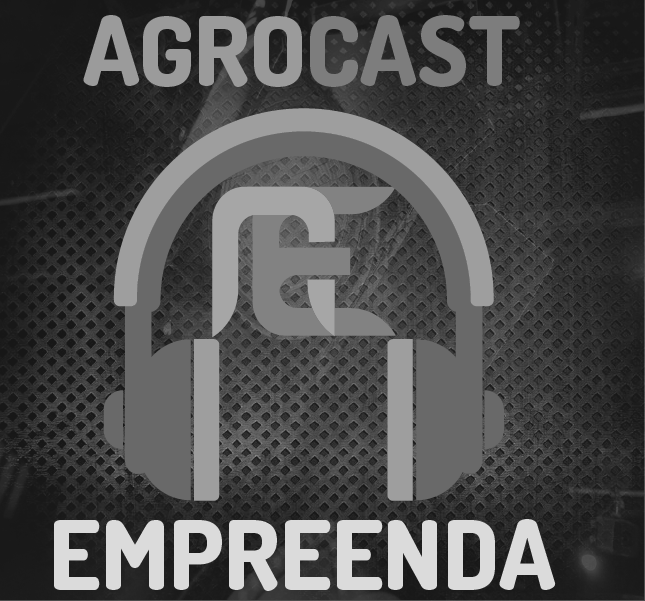
\includegraphics[scale=0.26]{Imagens/podcast_1.png}}
\qquad
\subfigure[ref2][Materiais de apoio produzidos]{\includegraphics[scale=0.2]{Imagens/podcast_2.jpg}}
\qquad
\subfigure[ref3][Materiais de apoio produzidos]{\includegraphics[scale=0.2]{Imagens/podcast_3.jpg}}
\qquad
\subfigure[ref3][Colaborador entrevistado]{\includegraphics[scale=0.2]{Imagens/podcast_4.jpg}}
\qquad
\subfigure[ref3][Colaborador entrevistado]{\includegraphics[scale=0.2]{Imagens/podcast_5.jpg}}
\qquad
\subfigure[ref3][Colaborador entrevistado]{\includegraphics[scale=0.2]{Imagens/podcast_6.jpg}}
\fonte{O Autor}.
\label{figura_podcast}
\end{figure}

\chapter{1º Workshop Empreenda Agro Sustentável}
\label{app:workshop_1}

\begin{figure}[H]
\FloatBarrier
\center
\caption{\textbf{1º Workshop Empreenda Agro Sustentável}}
\subfigure[ref1][Abertura do 1º Workshop ]{\includegraphics[scale=0.15]{Imagens/primeiro_dia_6.jpg}}
\qquad
\subfigure[ref2][Palestras do programa: 2º dia]{\includegraphics[scale=0.15]{Imagens/primeiro_dia_7.jpg}}
\qquad
\qquad
\subfigure[ref3][Palestras do programa: 2º dia]{\includegraphics[scale=0.2]{Imagens/primeiro_dia_1.jpg}}
\qquad
\subfigure[ref4][Palestras do programa: 2º dia]{\includegraphics[scale=0.2]{Imagens/primeiro_dia_2.jpg}}
\subfigure[ref5][Participantes do programa: 2º dia]{\includegraphics[scale=0.2]{Imagens/primeiro_dia_3.jpg}}
\qquad
\subfigure[ref6][Participantes do programa: 2º dia]{\includegraphics[scale=0.2]{Imagens/primeiro_dia_4.jpg}}
\fonte{O Autor}.
\label{figura_29_1}
\end{figure}


\chapter{2º Workshop Empreenda Agro Sustentável}
\label{app:workshop_2}

\begin{figure}[H]
\FloatBarrier
\center
\caption{\textbf{2º Workshop Empreenda Agro Sustentável}}
\subfigure[ref1][Participantes do programa: 1º dia ]{\includegraphics[scale=0.45]{Imagens/segundo_dia_1.jpg}}
\qquad
\subfigure[ref2][Participantes do programa: 2º dia]{\includegraphics[scale=0.07]{Imagens/segundo_dia_2.jpg}}
\qquad
\subfigure[ref3][Participantes do programa: 2º dia]{\includegraphics[scale=0.07]{Imagens/segundo_dia_3.jpg}}
\fonte{O Autor}.
\label{figura_50}
\end{figure}

\chapter{3º Workshop: Hackathon Empreenda Agro Sustentável}
\label{app:workshop_hackathon}


\begin{figure}[H]
\FloatBarrier
\center
\caption{\textbf{Hackathon Empreenda Agro Sustentável}}
\subfigure[ref1][Participantes do programa: Hackathon ]{\includegraphics[scale=0.43]{Imagens/terceiro_dia_1.jpg}}
\qquad
\subfigure[ref2][Participantes do programa: Hackathon]{\includegraphics[scale=0.20]{Imagens/terceiro_dia_3.jpg}}
\qquad
\subfigure[ref3][Participantes do programa: Hackathon]{\includegraphics[scale=0.20]{Imagens/terceiro_dia_4.jpg}}
\subfigure[ref4][Protótipos: Hackathon]{\includegraphics[scale=0.20]{Imagens/terceiro_dia_2.jpg}}
\qquad
\subfigure[ref5][Protótipos: Hackathon]{\includegraphics[scale=0.26]{Imagens/terceiro_dia_5.jpg}}
\fonte{O Autor}.
\label{figura_51}
\end{figure}

\chapter{4º Workshop: Demoday}
\label{app:workshop_demoday}

\begin{figure}[H]
\center
\FloatBarrier
\caption{\textbf{Demoday Empreenda Agro Sustentável}}
\subfigure[ref1][Evento  Demoday]{\includegraphics[scale=0.11]{Imagens/demoday_3.jpg}}
\qquad
\subfigure[ref2][Premiação simbólica]{\includegraphics[scale=0.2]{Imagens/demoday_premiacao.jpg}}
\qquad
\subfigure[ref3][Protótipos desenvolvidos: Tecno Coco]{\includegraphics[scale=0.112]{Imagens/demoday_15.jpg}}
\qquad
\subfigure[ref4][Protótipos desenvolvidos: MAMP]{\includegraphics[scale=0.2]{Imagens/demoday_12.jpg}}
\qquad
\subfigure[ref5][Protótipos desenvolvidos: Ranagro]{\includegraphics[scale=0.112]{Imagens/demoday_10.jpg}}
\qquad
\subfigure[ref6][Protótipos desenvolvidos: La Flora Pet]{\includegraphics[scale=0.12]{Imagens/demoday_6.jpg}}

\fonte{O Autor}.
\label{figura_35}
\end{figure}


\begin{landscape}
\includepdf[landscape=true,scale=0.87, pagecommand=\chapter{Cronograma}]{apendece/cronograma.pdf}
\end{landscape}


\begin{landscape}
\label{app:portfolio}

\includepdf[landscape=true,scale=0.70,pagecommand=\chapter{Portfólio Empreenda}]{apendece/portfolio_pb.pdf}
\end{landscape}
\includepdf[landscape=true,scale=0.80,pages={2-66},nup=2x2,pagecommand={}]{apendece/portfolio_pb.pdf}

% ----------------------------------------------------------
\end{apendicesenv}

%\begin{anexosenv}


% Imprime uma página indicando o início dos anexos
\partanexos

% ---
\chapter{Morbi ultrices rutrum lorem.}
% ---
\lipsum[30]

% ---
\chapter{Cras non urna sed feugiat cum sociis natoque penatibus et magnis dis
parturient montes nascetur ridiculus mus}
% ---

\lipsum[31]

% ---
\chapter{Fusce facilisis lacinia dui}
% ---

\lipsum[32]


\end{anexosenv}

\end{document}
